
% ----------------------------------------------------------------------
%                   LATEX TEMPLATE FOR PhD THESIS
% ----------------------------------------------------------------------

% based on Harish Bhanderi's PhD/MPhil template, then Uni Cambridge
% http://www-h.eng.cam.ac.uk/help/tpl/textprocessing/ThesisStyle/
% corrected and extended in 2007 by Jakob Suckale, then MPI-CBG PhD programme
% and made available through OpenWetWare.org - the free biology wiki


%: Style file for Latex
% Most style definitions are in the external file PhDthesisPSnPDF.
% In this template package, it can be found in ./Latex/Classes/
\documentclass[twoside,11pt]{Latex/Classes/PhDthesisPSnPDF}

\definecolor{darkgray}{rgb}{0.45,0.45,0.45}
\definecolor{lightgray}{gray}{0.8}
\definecolor{ultralightgray}{rgb}{0.95,0.95,0.95}
\definecolor{bluekeywords}{rgb}{0.13,0.13,1}
\definecolor{greencomments}{rgb}{0,0.5,0}
\definecolor{redstrings}{rgb}{0.9,0,0}



%: Macro file for L\begin{flushleft}\end{flushleft}atex
% Macros help you summarise frequently repeated Latex commands.
% Here, they are placed in an external file /Latex/Macros/MacroFile1.tex
% An macro that you may use frequently is the figuremacro (see introduction.tex)
% This file contains macros that can be called up from connected TeX files
% It helps to summarise repeated code, e.g. figure insertion (see below).

% insert a centered figure with caption and description
% parameters 1:filename, 2:title, 3:description and label
\newcommand{\figuremacro}[3]{
	\begin{figure}[htbp]
		\centering
		\includegraphics[width=1\textwidth]{#1}
		\caption[#2]{\textbf{#2} - #3}
		\label{#1}
	\end{figure}
}

% insert a centered figure with caption and description AND WIDTH
% parameters 1:filename, 2:title, 3:description and label, 4: textwidth
% textwidth 1 means as text, 0.5 means half the width of the text
\newcommand{\figuremacroW}[4]{
	\begin{figure}[htbp]
		\centering
		\includegraphics[width=#4\textwidth]{#1}
		\caption[#2]{\textbf{#2} - #3}
		\label{#1}
	\end{figure}
}

\newcommand{\figuremacroWR}[5]{
	\begin{figure}[htbp]
		\centering
		\includegraphics[width=#4\textwidth, angle=#5]{#1}
		\caption[#2]{\textbf{#2} - #3}
		\label{#1}
	\end{figure}
}

% inserts a figure with wrapped around text; only suitable for NARROW figs
% o is for outside on a double paged document; others: l, r, i(inside)
% text and figure will each be half of the document width
% note: long captions often crash with adjacent content; take care
% in general: above 2 macro produce more reliable layout
\newcommand{\figuremacroN}[3]{
	\begin{wrapfigure}{o}{0.5\textwidth}
		\centering
		\includegraphics[width=0.48\textwidth]{#1}
		\caption[#2]{{\small\textbf{#2} - #3}}
		\label{#1}
	\end{wrapfigure}
}

\newcommand{\figuremacroNW}[4]{
	\begin{wrapfigure}{o}{#4\textwidth}
		\centering
		\includegraphics[width=#4\textwidth]{#1}
		\caption[#2]{{\small\textbf{#2} - #3}}
		\label{#1}
	\end{wrapfigure}
}

% predefined commands by Harish
\newcommand{\PdfPsText}[2]{
  \ifpdf
     #1
  \else
     #2
  \fi
}

\newcommand{\IncludeGraphicsH}[3]{
  \PdfPsText{\includegraphics[height=#2]{#1}}{\includegraphics[bb = #3, height=#2]{#1}}
}

\newcommand{\IncludeGraphicsW}[3]{
  \PdfPsText{\includegraphics[width=#2]{#1}}{\includegraphics[bb = #3, width=#2]{#1}}
}

\newcommand{\InsertFig}[3]{
  \begin{figure}[!htbp]
    \begin{center}
      \leavevmode
      #1
      \caption{#2}
      \label{#3}
    \end{center}
  \end{figure}
}


%%% Local Variables: 
%%% mode: latex
%%% TeX-master: "~/Documents/LaTeX/CUEDThesisPSnPDF/thesis"
%%% End: 


\usepackage{Latex/StyleFiles/bytefield}
%\usepackage{Latex/StyleFiles/gantt}
\usepackage{Latex/StyleFiles/dpfloat}
\usepackage{pstricks}
\usepackage{pst-node}

\usepackage{tabularx}
\usepackage{graphicx}
\usepackage{epsfig}

\usepackage{subfig}
%\usepackage{subfigure}
\usepackage{wrapfig}
\usepackage{placeins}

\usepackage{listings}
%\usepackage{lscape}
\usepackage{pdflscape}
\usepackage{textpos}
\usepackage{rotating}
\usepackage{threeparttable}

% Paquets nececasir per les taules creades amb Gnumeric
\def\inputGnumericTable{}
%\usepackage[latin1]{inputenc}
\usepackage{color}
\usepackage{array}
\usepackage{longtable}
\usepackage{calc}
\usepackage{multirow}
\usepackage{hhline}
\usepackage{ifthen}

%\usepackage[section]{placeins}

\newcommand{\Monitor}{\emph{Monitor} }
\newcommand{\Controlador}{\emph{Controlador} }
\newcommand{\Actuador}{\emph{Actuador} }
\newcommand{\SensorActuador}{\emph{Sensor/Actuador} }
\newcommand{\Sensor}{\emph{Sensor} }
\newcommand{\Supervisor}{\emph{Supervisor} }
\newcommand{\DCSMonitor}{\textbf{DCSMonitor} }
\newcommand{\NECS} {\emph{NECS} }
\newcommand{\DI} {\emph{DI} }
\newcommand{\RTDruid} {\emph{RT-Druid} }
\newcommand{\Python} {\emph{Python} }
\newcommand{\C} {\emph{C} }
\newcommand{\Matlab} {MATLAB\textsuperscript{\textregistered} }
\newcommand{\QTCreator} {\emph{QTCreator} }
\newcommand{\PyQT} {\emph{PyQT4} }
\newcommand{\MplabX} {MPLAB\textsuperscript{\textregistered} X }
\newcommand{\pyuic} {\emph{pyuic4} }
\newcommand{\Ubuntu} {\emph{Ubuntu} }
\newcommand{\LiveCD} {\emph{Live CD} }
\newcommand{\FLEX} {\emph{FLEX} }
\newcommand{\Eclipse} {\emph{Eclipse} }
\newcommand{\PySerial} {\emph{PySerial} }
\newcommand{\Pylupdate} {\emph{Pylupdate4} }
\newcommand{\Qtlinguist} {\emph{QtLingüist} }
\newcommand{\Microchip} {\emph{Microchip} }

\renewcommand\lstlistlistingname{Índex de codis}
%\renewcommand\lstlistoflistings{%
%\begin{alwayssingle}
%\end{alwayssingle}
%}

\newcommand{\bitlabel}[2]{%
	\bitbox[]{#1}{%
		\raisebox{0pt}[4ex][0pt]{%
			\turnbox{45}{\fontsize{7}{7}\selectfont#2}%
			}%
	}%
}

\newcommand{\colorbitbox}[3]{%
	\rlap{\bitbox{#2}{\color{#1}\rule{\width}{\height}}}%
	\bitbox{#2}{#3}}
	

\lstloadlanguages{bash, Python, [ANSI]C, XML}

\lstnewenvironment{code_bash}[2]{
    \renewcommand\lstlistingname{\textbf{Codi Bash}}
    \lstset{caption={#1}, 
    label={#2},
    title={\colorbox{black!20}{\parbox{\dimexpr\linewidth-6pt\relax}{\centering \lstlistingname~\thelstlisting:\ \texttt{\detokenize{#1}}}}},
    language=bash, 
    basicstyle=\ttfamily,
	backgroundcolor=\color{ultralightgray},  % choose the background color. You must add \usepackage{color}
	commentstyle=\color{greencomments},
	keywordstyle=\color{bluekeywords},
	stringstyle=\color{redstrings},
	showspaces=false,               % show spaces adding particular underscores
	showstringspaces=false,         % underline spaces within strings
	breakatwhitespace=false,     % sets if automatic breaks should only happen at whitespace
	showtabs=false,                 % show tabs within strings adding particular underscores
	frame=b,                   % adds a frame around the code
	tabsize=2,                      % sets default tabsize to 2 spaces
	captionpos=b,                   % sets the caption-position to bottom
	breaklines=true,                % sets automatic line breaking
	xleftmargin=17pt,
	framexleftmargin=17pt,
	framexrightmargin=5pt,
	framexbottommargin=4pt,
	captionpos=top}
}{}

\lstnewenvironment{code_c}[2]{
    \renewcommand\lstlistingname{\textbf{Codi C}}
    \lstset{caption={#1}, 
    label={#2},
    title={\colorbox{black!10}{\parbox{\dimexpr\linewidth-6pt\relax}{\centering \lstlistingname~\thelstlisting:\ \texttt{\detokenize{#1}}}}},
    language=[ANSI]C, 
    basicstyle=\ttfamily,
	numbers=left,                   % where to put the line-numbers
	numberstyle=\footnotesize\color{gray},      % the size of the fonts that are used for the line-numbers
	stepnumber=1,                   % the step between two line-numbers. If it is 1 each line will be numbered
	numbersep=10pt,                  % how far the line-numbers are from the code
	backgroundcolor=\color{white},  % choose the background color. You must add \usepackage{color}
	commentstyle=\color{greencomments},
	keywordstyle=\color{bluekeywords},
	stringstyle=\color{redstrings},
	showspaces=false,               % show spaces adding particular underscores
	showstringspaces=false,         % underline spaces within strings
	breakatwhitespace=false,     % sets if automatic breaks should only happen at whitespace
	showtabs=false,                 % show tabs within strings adding particular underscores
	frame=b,                   % adds a frame around the code
	tabsize=2,                      % sets default tabsize to 2 spaces
	captionpos=b,                   % sets the caption-position to bottom
	breaklines=true,                % sets automatic line breaking
	xleftmargin=17pt,
	framexleftmargin=17pt,
	framexrightmargin=5pt,
	framexbottommargin=4pt,
	captionpos=top}
}{}

\lstnewenvironment{code_python}[2]{
    \renewcommand\lstlistingname{\textbf{Codi Python}}
    \lstset{caption={#1}, 
    label={#2},
    title={\colorbox{black!10}{\parbox{\dimexpr\linewidth-6pt\relax}{\centering \lstlistingname~\thelstlisting:\ \texttt{\detokenize{#1}}}}},
    language=python, 
    basicstyle=\ttfamily,
	numbers=left,                   % where to put the line-numbers
	numberstyle=\footnotesize\color{gray},      % the size of the fonts that are used for the line-numbers
	stepnumber=1,                   % the step between two line-numbers. If it is 1 each line will be numbered
	numbersep=10pt,                  % how far the line-numbers are from the code
	backgroundcolor=\color{white},  % choose the background color. You must add \usepackage{color}
	commentstyle=\color{greencomments},
	keywordstyle=\color{bluekeywords},
	stringstyle=\color{redstrings},
	showspaces=false,               % show spaces adding particular underscores
	showstringspaces=false,         % underline spaces within strings
	breakatwhitespace=false,     % sets if automatic breaks should only happen at whitespace
	showtabs=false,                 % show tabs within strings adding particular underscores
	frame=b,                   % adds a frame around the code
	tabsize=2,                      % sets default tabsize to 2 spaces
	captionpos=b,                   % sets the caption-position to bottom
	breaklines=true,                % sets automatic line breaking
	xleftmargin=17pt,
	framexleftmargin=17pt,
	framexrightmargin=5pt,
	framexbottommargin=4pt,
	captionpos=top,
	morekeywords={SIGNAL}}
}{}


\lstnewenvironment{code_xml}[2]{
    \renewcommand\lstlistingname{\textbf{Codi XML}}
    \lstset{caption={#1}, 
    label={#2},
    title={\colorbox{black!10}{\parbox{\dimexpr\linewidth-6pt\relax}{\centering \lstlistingname~\thelstlisting:\ \texttt{\detokenize{#1}}}}},
    language=XML, 
    basicstyle=\ttfamily,
	numbers=left,                   % where to put the line-numbers
	numberstyle=\footnotesize\color{gray},      % the size of the fonts that are used for the line-numbers
	stepnumber=1,                   % the step between two line-numbers. If it is 1 each line will be numbered
	numbersep=10pt,                  % how far the line-numbers are from the code
	backgroundcolor=\color{white},  % choose the background color. You must add \usepackage{color}
	commentstyle=\color{greencomments},
	keywordstyle=\color{bluekeywords},
	stringstyle=\color{redstrings},
	showspaces=false,               % show spaces adding particular underscores
	showstringspaces=false,         % underline spaces within strings
	breakatwhitespace=false,     % sets if automatic breaks should only happen at whitespace
	showtabs=false,                 % show tabs within strings adding particular underscores
	frame=b,                   % adds a frame around the code
	tabsize=2,                      % sets default tabsize to 2 spaces
	captionpos=b,                   % sets the caption-position to bottom
	breaklines=true,                % sets automatic line breaking
	xleftmargin=17pt,
	framexleftmargin=17pt,
	framexrightmargin=5pt,
	framexbottommargin=4pt,
	captionpos=top,
	morekeywords={SIGNAL}}
}{}

%: ----------------------------------------------------------------------
%:                  TITLE PAGE: name, degree,..
% ----------------------------------------------------------------------
% below is to generate the title page with crest and author name

%if output to PDF then put the following in PDF header
\ifpdf  
    \pdfinfo { /Title  (Design of a platform to test distributed control systems)
               /Creator (TeX)
               /Producer (pdfTeX)
               /Author (Miquel Perello Nieto miquel.perello.nieto@fib.upc.edu)
               /CreationDate (D:DDMMYYYYhhmmss)  %format D:YYYYMMDDhhmmss
               /ModDate (D:DDMMYYYYhhmm)
               /Subject (xyz)
               %/Directors (Josep Pep, Manel Velasco)
               %Directors: Josep Maria Fuertes Armengol y Manel Velasco Garcia
               /Keywords (add, your, keywords, here) }
    \pdfcatalog { /PageMode (/UseOutlines)
                  /OpenAction (fitbh)  }
\fi


\title{Design of a platform to test distributed control systems}



% ----------------------------------------------------------------------
% The section below defines www links/email for author and institutions
% They will appear on the title page of the PDF and can be clicked
\ifpdf
  \author{\href{mailto:miquel.perello.nieto@fib.upc.edu}{Miquel Perello Nieto}}
%  \cityofbirth{born in XYZ} % uncomment this if your university requires this
%  % If city of birth is required, also uncomment 2 sections in PhDthesisPSnPDF
%  % Just search for the "city" and you'll find them.
  \collegeordept{\href{http://www.fib.upc.edu}{Facultat d'Informàtica de Barcelona}}
  \university{\href{http://www.upc.edu}{Universitat Politècnica de Catalunya}}
  %\director{\href{mailto:miquel.perello.nieto@fib.upc.edu}{Josep Maria Fuertes Armengol}}
  %\codirector{\href{mailto:miquel.perello.nieto@fib.upc.edu}{Manel Velasco Garcia}}
  

  % The crest is a graphics file of the logo of your research institution.
  % Place it in ./0_frontmatter/figures and specify the width
  \crest{
\includegraphics[width=5cm]{logoUPC}}
  
% If you are not creating a PDF then use the following. The default is PDF.
\else
  \author{Miquel Perello Nieto}
%  \cityofbirth{born in XYZ}
  \collegeordept{Facultat d'Informàtica de Barcelona}
  \university{Universitat Politècnica de Catalunya}
  \crest{
\includegraphics[width=5cm]{logoUPC}}
\fi

\renewcommand{\submittedtext}{Memòria de Projecte Final de Carrera}
\degree{Enginyeria Tècnica en Informàtica de Sistemes}
\degreedate{Gener 2011}


% ----------------------------------------------------------------------
       
% turn of those nasty overfull and underfull hboxes
\hbadness=10000
\hfuzz=50pt


%: --------------------------------------------------------------
%:                  FRONT MATTER: dedications, abstract,..
% --------------------------------------------------------------

\begin{document}

%\language{english}

% sets line spacing
\renewcommand\baselinestretch{1.2}
\baselineskip=18pt plus1pt


%: ----------------------- generate cover page ------------------------

\maketitle  % command to print the title page with above variables


%: ----------------------- cover page back side ------------------------
% Your research institution may require reviewer names, etc.
% This cover back side is required by Dresden Med Fac; uncomment if needed.

\newpage
\vspace{10mm}
1. Directors: Josep Maria Fuertes Armengol y Manel Velasco Garcia

\vspace{10mm}
2. President: Pere Marés Martí

\vspace{10mm}
3. Vocal: Robert Lukas Mario Nieuwenhuis

\vspace{20mm}
Dia de lectura:

\vspace{20mm}
\hspace{70mm}Signatura del tribunal del PFC:



%: ----------------------- abstract ------------------------

% Your institution may have specific regulations if you need an abstract and where it is to be placed in the document. The default here is just after title.


% Thesis Abstract -----------------------------------------------------


%\begin{abstractslong}    %uncommenting this line, gives a different abstract heading
\begin{abstracts}        %this creates the heading for the abstract page

El propòsit d'aquesta memòria és el d'explicar la importància que tenen els Sistemes Distribuïts de Control, i els problemes que sorgeixen al controlar sistemes dinàmics en temps real.

Per tal de mostrar això, des del departament de ESAII s'han dissenyat una sèrie de laboratoris amb els quals els estudiants poden entendre i resoldre els problemes que d'aquest tema se'n deriven.

Amb la realització d'aquest projecte es va procurar donar un pas més amb aquest propòsit i d'aquesta manera es va dissenyar un sistema de monitorització i control sobre les comunicacions entre diferents dispositius que formen llaços de control en el medi compartit d'un bus CAN.

La memòria és el reflex de les tecnologies que es troben en aquests Sistemes i els programes que s'han creat i/o modificat per controlar-los. Entre ells s'en destaca el programa \DCSMonitor, creat íntegrament en aquest projecte, i dissenyat modularment per tal de servir com a base en qualsevol entorn futur.

Igualment per la part dels dispositius del bus CAN, els quals amb un disseny escalable realitzat en el projecte, poden servir per una infinitud d'objectius nous, i per la realització de projectes enfocats a aquest tipus de sistemes.

Per tant amb la finalització d'aquest projecte, queden obertes moltes possibilitats, i s'espera que tant en l'entorn acadèmic com en l'industrial, es puguin utilitzar les seves idees.

\emph{Tot el material emprat en la realització d'aquest projecte pot ser consultat en el repositori \href{http://code.google.com/p/pfc-platform-test/}{http://code.google.com/p/pfc-platform-test/}}

\emph{Per la realització de la pressent memòria ha estat emprat un template de LaTeX el qual es pot trobar en la bibliografia \cite{Korten2010}}

\end{abstracts}
%\end{abstractlongs}


% ---------------------------------------------------------------------- 


% The original template provides and abstractseparate environment, if your institution requires them to be separate. I think it's easier to print the abstract from the complete thesis by restricting printing to the relevant page.
% \begin{abstractseparate}
%   
% Thesis Abstract -----------------------------------------------------


%\begin{abstractslong}    %uncommenting this line, gives a different abstract heading
\begin{abstracts}        %this creates the heading for the abstract page

El propòsit d'aquesta memòria és el d'explicar la importància que tenen els Sistemes Distribuïts de Control, i els problemes que sorgeixen al controlar sistemes dinàmics en temps real.

Per tal de mostrar això, des del departament de ESAII s'han dissenyat una sèrie de laboratoris amb els quals els estudiants poden entendre i resoldre els problemes que d'aquest tema se'n deriven.

Amb la realització d'aquest projecte es va procurar donar un pas més amb aquest propòsit i d'aquesta manera es va dissenyar un sistema de monitorització i control sobre les comunicacions entre diferents dispositius que formen llaços de control en el medi compartit d'un bus CAN.

La memòria és el reflex de les tecnologies que es troben en aquests Sistemes i els programes que s'han creat i/o modificat per controlar-los. Entre ells s'en destaca el programa \DCSMonitor, creat íntegrament en aquest projecte, i dissenyat modularment per tal de servir com a base en qualsevol entorn futur.

Igualment per la part dels dispositius del bus CAN, els quals amb un disseny escalable realitzat en el projecte, poden servir per una infinitud d'objectius nous, i per la realització de projectes enfocats a aquest tipus de sistemes.

Per tant amb la finalització d'aquest projecte, queden obertes moltes possibilitats, i s'espera que tant en l'entorn acadèmic com en l'industrial, es puguin utilitzar les seves idees.

\emph{Tot el material emprat en la realització d'aquest projecte pot ser consultat en el repositori \href{http://code.google.com/p/pfc-platform-test/}{http://code.google.com/p/pfc-platform-test/}}

\emph{Per la realització de la pressent memòria ha estat emprat un template de LaTeX el qual es pot trobar en la bibliografia \cite{Korten2010}}

\end{abstracts}
%\end{abstractlongs}


% ---------------------------------------------------------------------- 

% \end{abstractseparate}


%: ----------------------- tie in front matter ------------------------

\frontmatter
% Thesis Dedictation ---------------------------------------------------

\begin{dedication} %this creates the heading for the dedication page

Dedicat al meu pare, per haver-me deixat llibertat en els estudis, permetrem decidir equivocar-me i aprendre dels meus errors, i tot i així no deixar d'ajudar-me en tot moment.

A la meva família, per ensenyar-me cadascun una cosa nova a la seva manera.

I a la meva mare.

\end{dedication}

% ----------------------------------------------------------------------

% Thesis Acknowledgements ------------------------------------------------


%\begin{acknowledgementslong} %uncommenting this line, gives a different acknowledgements heading
\begin{acknowledgements}      %this creates the heading for the acknowlegments

Agraeixo al meu tutor Pep Fuertes que un dia es deixés veure en una conferencia sobre grans telescopis, i em captivés des d' aquell instant ja fa algun any. 
Que el tornés a trobar accidentalment buscant un Projecte Final de Carrera, proposant ampliar el laboratori de Sistemes Distribuïts de Control i que jo acceptés sense saber ven bé que eren, perquè forçosament havia de ser alguna cosa molt interessant. I perquè encara que semblés tenir les coses descontrolades, realment guardés un control absolut de tot.

També haig de donar les gràcies a l'altre tutor Manel Velasco, per poder-me dedicar el temps suficient i just per tirar endavant el projecte; per fer fàcils les coses que semblaven difícils, per ensenyar-me una infinitud de tecnologies desconegudes per mi, per ferme pensar en algun moment que ell era l'informàtic, per ajudar-me en els moments que estava perdut, i per tranquil·litzar-me quan pensava que no m'en sortiria.

Gracies també al Pau Martí per estar donant suport sense la seva presencia física per e-mails i una trucada sorpresa. 

Sobretot haig de donar les gracies a la meva novia Virgínia Rodríguez, per obligar-me a aparcar el projecte de tant en tant, i treure'm literalment de casa per descansar. I per comprendre en certs moments que realment de tant en tant s'ha de fer feina.

Gracies també a la Pantera i al Kobu, per fer-me companyia en els moments en els que estava sol en el projecte, i no demanar rés a canvi (bé... una mica de pinso i aigua sí...).
\begin{flushright}
\begin{minipage}[l]{0.5\linewidth}
\emph{"en definitiva gracies a tothom, perquè sense ningú res d'això tindria cap sentit"}
\end{minipage}
\end{flushright}

\end{acknowledgements}
%\end{acknowledgmentslong}

% ------------------------------------------------------------------------





%: ----------------------- contents ------------------------

\setcounter{secnumdepth}{3} % organisational level that receives a numbers
\setcounter{tocdepth}{3}    % print table of contents for level 3
\tableofcontents            % print the table of contents
% levels are: 0 - chapter, 1 - section, 2 - subsection, 3 - subsection


%: ----------------------- list of figures/tables ------------------------

\listoffigures	% print list of figures

\listoftables  % print list of tables


\lstlistoflistings
\addcontentsline{toc}{chapter}{Índex de codis}

%: ----------------------- glossary ------------------------

% Tie in external source file for definitions: /0_frontmatter/glossary.tex
% Glossary entries can also be defined in the main text. See glossary.tex
% this file is called up by thesis.tex
% content in this file will be fed into the main document

% Glossary entries are defined with the command \nomenclature{1}{2}
% 1 = Entry name, e.g. abbreviation; 2 = Explanation
% You can place all explanations in this separate file or declare them in the middle of the text. Either way they will be collected in the glossary.

% required to print nomenclature name to page header
\markboth{\MakeUppercase{\nomname}}{\MakeUppercase{\nomname}}


% ----------------------- contents from here ------------------------

% chemicals
\nomenclature{DCSMonitor}{Nom del programa creat en aquest projecte per rebre totes les dades monitoritzades presents en el bus CAN. Ve de les sigles en Anglès de \textit{Distributed Control Systems Monitor} (Monitor de Sistemes Distribuïts de Control)}

\nomenclature{DCS}{Sigles en Anglès de \textit{Distributed Control System}  (Sistema Distribuït de Control); són sistemes de control aplicats generalment en sistemes de fabricació, o qualsevol tipus de sistemes dinàmics, en els quals els elements de control no són centrals sinó que estan distribuïts en el sistema a més cada component del subsistema està connectat als demés mitjançant una xarxa.}

\nomenclature{CAN}{Sigles en Anglès de \textit{Controller Area Network}; És un protocol de comunicacions desenvolupat per la firma alamanya Robert Bosch GmbH, basat en una topologia en bus per la transmissió de missatges en entorns distribuïts.}

\nomenclature{RTOS}{Sigles en Anglès de \textit{Real-Time Operating System} (Sistema Operatiu en Temps Real); es diu dels Sistemes Operatius dissenyats per atendre aplicacions en temps real. La principal característica d'aquests SO és el nivell de precisió en els temps d'execució de cada una de les tasques que ha de realitzar.}

\nomenclature{.elf}{Sigles en Anglès de \textit{Executable and Linkable Format} (Format Enllaçable i Executable ); és un format de fitxers per executables, codi obert, biblioteques compartides i bolcat de memòria. Va ser dissenyat per \emph{Unix System Laboratories}, i en principi va ser desenvolupat per plataformes de 32 bits, encara que actualment s'utilitza en varietat de plataformes.}

\nomenclature{.svg}{Sigles en Anglès de \textit{Scalable Vector Graphics} (Gràfics Vectorials Escalables); és una especificació per descriure gràfics vectorials bidimensionals, tant estàtics com dinàmics, en format XML.}

\nomenclature{PIC}{Sigles en Anglès de \textit{Peripheral Interface Controller} (Controlador d'Interficie de Periféric); són una familia de microcontroladors de tipus RISC fabricats per \emph{Microchip Technology Inc.} originalment creats per la divisió de microelectrónica de General Instruments.}

\nomenclature{dsPIC33FJ256MC710}{Model de microcontrolador de la casa \emph{Microchip} caracteritzat per ser de la família dels dsPIC i per comptar amb multitud d'utilitats en sistemes distribuïts.}

\nomenclature{dsPIC}{Família de microcontroladors fabricats per la casa \emph{Microchip} caracteritzat per comptar amb bus de dades inherent de 16 bits, i per incorporar varies operacions de DSP implementades en hardware.}

\nomenclature{DSP}{Sigles en Anglès de \textit{Digital Signal Processor} (Processador de Senyals Digitals); són microprocesadors especialitzats amb una arquitectura optimitzada per el tractament ràpid de senyals digitals.}

\nomenclature{Llaç de Control}{En els sistemes distribuïts de control s'anomena d'aquesta manera a un grup de dispositius que formen part del control d'algun proces, en el cas del nostre laboratori aquests grups estan formats per un \Controlador, un \Sensor i un \Actuador.}

\nomenclature{Microcontrolador}{Es un circuit integrat programable, capaç d'executar les ordres gravades en la seva memòria. Està composat per varis blocs funcionals, els quals compleixen una tasca concreta. Un microcontrolador conté al seu interior les tres unitats funcionals principals de un computador: unitat central de processament, memòria i perifèrics d'entrada i sortida.}

\nomenclature{Microprocesador}{Els microprocesadors compten amb les funcions d'una CPU (Unitat Central de Procesament) en un o varis circuits integrats.}

\nomenclature{Controlador}{El controlador en sistema distribuït de control és l'encarregat de calcular el valor a donar al actuador per tal de aconseguir un senyal desitjat.}

\nomenclature{Sensor}{El sensor en un sistema distribuït de control és l'encarregat de prendre els valors de sortida del sistema, per tal de oferir-li al controlador.}

\nomenclature{Actuador}{L'actuador en un sistema distribuït de control és l'encarregat de assignar el valor calculat pel controlador a l'entrada del circuit a controlar.}

\nomenclature{Supervisor}{El supervisor en un sistema distribuït de control és el dispositiu que ens dona els valors necessaris del sistema per saber el seu estat.}

\nomenclature{Monitor}{El monitor es un dispositiu que hem afegit en el nostre laboratori i en el sistema distribuït de control que s'encarrega de monitoritzar el bus del sistema capturant la informació demanada, i poden interferir en el sistema per veure la resposta dels diferents controls.}

\nomenclature{IDE}{Sigles en Anglès de \textit{Integrated Development Environment} (Entorn de Desenvolupament Integrat); és un programa informàtic composat per un conjunt d'eines de programació en un o varis llenguatges de programació i dedicat a ajudar en les tasques habituals de programació.}

\nomenclature{.ui}{Sigles en Anglès de \textit{User Interface} (Interficie d'usuari'); és un format de fitxers creat per la casa QT, i amb informació necessària per muntar la interfície visual d'un programa.}

\nomenclature{API}{Sigles en Anglès de \textit{Application Programming Interface} (Interfície de Programació d'Aplicacions); és un conjunt de declaracions amb el propòsit de ser usades per un altre programa com una capa d'abstracció.}

\nomenclature{DMA}{Sigles en Anglès de \textit{Direct Memory Acces} (Accés Directe a Memòria); és un mètode que permet a certs tipus de circuits integrats accedir a la memòria d'aquests per llegir i escriure independentment de la CPU principal.}

\nomenclature{PWM}{Sigles en Anglès de \textit{Pulse-Width Modulation} (Modulació per amplària d'impuls); aquesta és una tècnica en la qual es modifica el cicle de treball d'un senyal periòdic (una ona sinusoïdal o ona quadrada, per exemple), ja sigui per transmetre informació a través d'un canal de comunicacions o per controlar la quantitat d'energia que s'envia a una càrrega.}

\nomenclature{WBS}{Sigles en Anglès de \textit{Work Breakdown Structure} (Estructura de Descomposició de Treball); en gestió de projectes es una descomposició jeràrquica orientada al entregable, del treball a ser realitzat per l'equip del projecte per cumplir amb els objectius d'aquest.}

\nomenclature{Mutex}{De l'Anglès \textit{Mutual Exclusión} (Zona d'exclusió mutua); tipus d'algoritmes utilitzats en la programació concurrent per evitar l'us simultani dels recursos, com variables globals, per fragments de codi coneguts de manera comú com zones crítiques.}


\nomenclature{.ts}{De l'Anglès \textit{Translation files} (Fitxers de traducció); Tipus d'extensió de fitxers utilitzats per QtLingüist per crear traduccions dels textos d'un programa.}

\nomenclature{.qm}{Extensió d'un tipus de fitxers que utilitza la llibreria PyQT4 per traduir textos.}

\nomenclature{SAE}{Sigles en Anglès de \textit{Society of Automotive Engineers} (Societat d'Enginyers Automotrius); és l'organització enfocada a la mobilitat dels professionals en l'enginyeria aeroespacial, automoció, i industries comercials especialitzades en la construcció de vehicles.}

\nomenclature{IPS}{Sigles en Anglès de \textit{Instructions Per Second} (Instruccions Per Segon); és una mesura de velocitat d'un processador. Indica el nombre d'instruccions que la CPU pot executar en un segon.} 

\nomenclature{OSEK/VDX}{Sigles en Alemà de \textit{Offene Systeme und deren Schnittstellen für die Elektronik in Kraftfahrzeugen} (Sistemes oberts i les seves interfícies per la electrònica en automòbils); és un estandart que especifica el Sistema Operatiu integrat incloent una pila per comunicacions i un protocol per l'administració de xarxes per sistemes empotrats en automòbils.} 

\nomenclature{XML}{De l'Anglès \textit{eXtensible Markup Language} (Llenguatge de Marques Extensibles); és un metallenguatge d'etiquetes, desenvolupat per el \emph{World Wide Web Consortium (W3C)} que permet definir la gramàtica de llenguatges específics.} 

 

%\begin{multicols}{2} % \begin{multicols}{#columns}[header text][space]
\begin{footnotesize} % scriptsize(7) < footnotesize(8) < small (9) < normal (10)

\printnomenclature[1.5cm] % [] = distance between entry and description
\label{nom} % target name for links to glossary

\end{footnotesize}
%\end{multicols}



%: --------------------------------------------------------------
%:                  MAIN DOCUMENT SECTION
% --------------------------------------------------------------

% the main text starts here with the introduction, 1st chapter,...
\mainmatter

\renewcommand{\chaptername}{} % uncomment to print only "1" not "Chapter 1"


%: ----------------------- subdocuments ------------------------

% Parts of the thesis are included below. Rename the files as required.
% But take care that the paths match. You can also change the order of appearance by moving the include commands.


% this file is called up by thesis.tex
% content in this file will be fed into the main document

%: ----------------------- introduction file header -----------------------
\chapter{Introducció}\label{cap:int}

% the code below specifies where the figures are stored
\ifpdf
    \graphicspath{{1_introduction/figures/PNG/}{1_introduction/figures/PDF/}{1_introduction/figures/}}
\else
    \graphicspath{{1_introduction/figures/EPS/}{1_introduction/figures/}}
\fi

% ----------------------------------------------------------------------
%: ----------------------- introduction content ----------------------- 
% ----------------------------------------------------------------------



%: ----------------------- HELP: latex document organisation
% the commands below help you to subdivide and organise your thesis
%    \chapter{}       = level 1, top level
%    \section{}       = level 2
%    \subsection{}    = level 3
%    \subsubsection{} = level 4
% note that everything after the percentage sign is hidden from output

Aquesta memòria pretén reflectir de manera clara i entenedora el procés que s'ha seguit per dur a terme un laboratori de "Sistemes Distribuïts de Control" (a partir d'ara SDC), així com els problemes que hagin pogut sorgir en el transcurs del projecte.

La realització d'aquest laboratori ha comportat l'adquisició d'una visió profunda del que es pretén ensenyar des del departament de ESAII \index{ESAII} de la UPC en el tema dels SDC \index{SDC}.

Per tant en el transcurs d'aquesta memòria s'anirà endinsant en aquest tipus de sistemes, es coneixeran quines són algunes de les tecnologies base que els conformen, els problemes que en elles esdevenen, i solucions a algunes d'aquestes qüestions.

Amb tot això es podrà tenir una idea més clara del motiu de la realització d'aquest projecte i les portes que a partir d'aquest projecte queden obertes.

A més es poden veure com a apèndix les dues guies realitzades en aquest projecte, una per la preparació de l'entorn de desenvolupament i posterior utilització del laboratori. I una altre per l'ús del LiveCD \index{LiveCD} pel desenvolupament pràctic del laboratori.

%====================================================================================%
% Estructuració de la memòria
%====================================================================================%
\section{Estructuració de la memòria}\label{cap:int:estruct}

En aquesta secció mirarem de donar una visió global de la memòria, perquè sigui fàcil de ser consultada, i d'aquesta manera tenir en tot moment una idea de on es pot trobar qualsevol qüestió. Per tant començar indicant que aquesta memòria ha estat escrita seguint l'ordre cronològic que esdevé al desenvolupar i portar a terme un projecte.

D'aquesta manera primerament ens trobem  amb el capítol de Introducció (capítol \ref{cap:int}), en el qual podem veure resumidament de que tracta el projecte, quines són les raons de la seva elecció i perquè aquest projecte és important (secció Motivació \ref{cap:int}), quin era l'objectiu d'aquest projecte amb les limitacions del temps que tenia (secció Abast \ref{cap:int:ab}), i de quina manera es va organitzar el temps per realitzar-lo, i reorganitzar-lo en el moment que això va caldre (secció Planificació \ref{cap:int:plan}).

Un cop es té una idea global ben clara dels objectius d'aquest projecte, és el moment d'aprofundir una mica en les tecnologies que en aquest es toquen, per tant tot seguit veurem el capítol Tecnologia (capítol \ref{cap:tec}). Aquest capítol l'hem dividit en tres parts per tipus de tecnología. 

En la primera part parlarem sobre els dispositius físics (secció Hardware \ref{cap:tec:hard}) en la que explicarem quines plaques s'utilitzen al laboratori per fer els controls (secció FLEX \ref{cap:tec:hard:flex}), tot seguit explicarem quin es el nucli d'aquestes plaques (secció dsPIC33FJ256MC710 \ref{cap:tec:hard:dspic}), quin integrat ens permet fer d'intermediari per les comunicacions CAN (secció MCP2551 \ref{cap:tec:hard:mcp2551}), i amb quin dispositiu podem programar qualsevol microcontrolador de la casa Microchip (secció ICD2/3 \ref{cap:tec:hard:icd}).

En la segona part parlarem del software que s'ha usat per elaborar el projecte i el laboratori (secció Software \ref{cap:tec:soft}), en ella parlarem del IDE que hem utilitzat per programar tant el codi en python del programa \DCSMonitor com el codi del Sistema Operatiu en Temps Real Erika (secció \Eclipse \ref{cap:tec:soft:eclipse}), el programa que hem utilitzat per programar els dispositius (secció \MplabX \ref{cap:tec:soft:mplab}), del IDE que hem usat per crear les interficies del programa \DCSMonitor (secció QtCreator \ref{cap:tec:soft:qtcreator}), de la eina que ens facilita crear els fitxers de traducció del programa \DCSMonitor (secció QtLingüist \ref{cap:tec:soft:qtlinguist}), i per ultim el Sistema Operatiu en Temps Real que formen el cervell dels dispositius del bus CAN (secció ERIKA Enterprise \ref{cap:tec:soft:erika}).

Per ultim farem una pinzellada a alguns protocols que hem d'entendre per poder ser conscients dels problemes i solucions que atorga cadascun (secció Protocols de comunicació \ref{cap:tec:prot}), així que comencem per el més important en els Sistemes Distribuits de Control amb el qual tots els dispositius es troben ben comunicats (secció CAN ref{cap:tec:prot:can}), tot seguit el que ens permet rebre a l'ordinador tot el que está succein al bus CAN (secció Serie via RS232 \ref{cap:tec:prot:rs232}), i per finalitzar el tipus de topologia en el que es troben tots els dispositius del laboratori (secció Topologia en bus \ref{cap:tec:prot:bus})

A partir d'aquest punt comença a aparèixer les noves idees que aporta el projecte, en el capítol Disseny del laboratori (capítol \ref{cap:dis}) primerament s'explicarà que s'ensenya actualment en el laboratori, i quines són les eines que s'utilitzen (secció Resum del laboratori actual ,\ref{cap:dis:resum}). Tot seguit amb la secció Disseny del Nou laboratori ,\ref{diss:nou}, es plantegen quins són els problemes que es volen resoldre, i com s'aconsegueix en alguns temes del laboratori com són la creació de la interfície (secció \ref{cap:dis:visual}), els problemes amb els identificadors que s'han d'assignar als diferents dispositius del bus CAN (secció \ref{cap:dis:idCAN}), la comunicació entre el programa \DCSMonitor (programa que corre a l'ordinador) i els diferents dispositius mitjançant comunicació serie per RS232 (secció \ref{cap:dis:comSer}), el disseny que es va pensar pel mostreig de les gràfiques en temps real (secció \ref{cap:dis:graph}) i el mètode escollit per poder fer el programa multilingüe i fàcilment ampliable (secció \ref{cap:dis:idi}).

Per altre banda tenim el \emph{com} es va portar a terme el sistema dissenyat anteriorment, d'aquesta manera en el capítol Implementació del laboratori (capítol \ref{cap:imp}) toca el torn d'explicar la metodología per fer realitat el laboratori plantejat. 
Primerament ens centrarem en el programa d'ordinador \DCSMonitor (secció \ref{cap:imp:dcs}) començant per la part visual del programa (la interfície en la secció \ref{cap:imp:visual}), seguint amb la implementació de la comunicació sèrie (secció \ref{cap:imp:com:serie}). Després una de les parts més importants que és la generació de les gràfiques en temps real (secció \ref{cap:imp:gen:graph}); gracies a les quals podem avaluar la bondat dels controls que hi ha al bus CAN, l'exportació d'aquestes gráfiques en diferents formats (secció \ref{cap:imp:exp:graph}) i finalment la integració de la multiculturalitat, o creació de la interficie multilingüe (secció \ref{cap:imp:idi}).
La part dels dispositius no és menys important, i per tant té també la seva secció d'implementació (\ref{lab:imp:dspic:monitor}), en ella s'expliquen els mètodes que s'han usat per portar a terme les comunicacions series per RS232 (secció \ref{lab:imp:dspic:monitor:serie}), i tot el relacionat amb les comunicacions CAN (secció \ref{lab:imp:dspic:can}).


Al acabar el projecte, ha estat possible comprovar les hores reals que si han dedicat, i per tant fer càlculs dels preus del material i de la ma d'obra. Per tant tot seguit ve el capítol Anàlisi econòmic \ref{cap:eco}, on es poden veure un desglos del preu del projecte.

Després venen les conclusions ,\ref{cap:conc}, on es deixa constància de quins han estat els objectius aconseguits, possibles ampliacions que pot tindre aquest projecte, i una visió general després d'haver realitzat el projecte.


Com apèndix tenim les dues guies que s'han elavorat per l'execució del laboratori en un sistema Linux (\Ubuntu) \ref{cap:lab_gui}, i una guia d'us del \LiveCD creat en aquest projecte, per tenir en marxa tot aquest sistema en 6 minuts (més larrancada de l'ordinador) \ref{cap:cd_gui}.


%====================================================================================%
% Motivació
%====================================================================================%
\section{Motivació}\label{cap:int:mot}

Moltes són les raons per les quals aquest projecte va ser començat i posteriorment tirat endavant. Primerament perquè els sistemes electrònics empotrats són a tot arreu; caixers automàtics, impressores, calculadores, rellotges, equips mèdics, telèfons mòbils... Però què és un sistema si no pot ser consultat en temps real? De que serveix un sistema electrònic aïllat del que no es pot treure cap tipus d'informació a l'instant? Actualment quasi tots els sistemes procuren d'una o altre manera estar en constant comunicació, volem saber en cada moment quin és l'estat d'alguna lectura, si hi ha algun problema en algun aparell que hagi de ser revisat, si el ABS del cotxe funcionarà en el moment que toqui, si el cafè de després de les postres ja és ben calent... 
 
Per tant l'aparició dels sistemes distribuïts es veu forçada a sorgir de les mancances que tenien els sistemes totalment autònoms, i així esdevenir poc a poc una realitat actual. Peró aquesta aparició no sorgeix i esdevé una realitat idíl·lica en el moment de néixer, sinó que junt amb ella apareixen nous problemes e inconvenients; la concurrència de tots els sistemes comunicats és un problema greu, i no tots els sistemes són igual de crítics; n'hi ha que només donen lectures periòdiques sense massa importància, però també n'hi ha que salven vides.

Un clar exemple de tot això és el protocol de comunicació CAN, desenvolupat fa només 3 dècades; aquest va començar a l'any 1983 per \emph{Robert Bosch GmbH} i va ser oficialment alliberat al 1986 per la Societat d'Enginyers Automotrius (SAE, Society of Automotive Engineers). Va ser principalment creat per la industria automòbil, gracies a la qual es van poder posar molts dels sistemes de seguretat que hi ha actualment als cotxes; gracies als quals es salven moltes vides; però que actualment és usat en molts altres sectors, com poden ser equips mèdics, controls industrials, entorns aeroespacials, marítims, etc.

Aquesta és una de les raons per les quals s'ha escollit la realització d'aquest projecte. Perquè són sistemes reals, i que encara no estan perfeccionats; i això és així no perquè no siguin importants, sinó perquè pertanyen a una branca de la tecnologia que encara està en constant evolució.

Per tant, espero que es vegi la importància que aquest projecte porta darrera, i que la realització d'aquest no tanca cap porta, sinó que deixa obert un camí molt llarg per explorar.


%====================================================================================%
% Abast
%====================================================================================%
\section{Abast}\label{cap:int:ab}

Aquest projecte pot ser continuat, per tant cal indicar que amb la limitació de temps amb la que conta el projecte (relativa al nombre de crèdits), en algun moment s'ha hagut de posar una fita. Per tant s'exposa en aquest apartat els objectius que s'han proposat aconseguir.


%====================================================================================%
% Objectius
%====================================================================================%
\subsection{Objectius}% subsection headings are again smaller than section names
% lead
Abans  d'escollir aquest projecte es van plantejar alguns dels objectius que aquest hauria de complir, però un cop començat es van anar refinant i ampliant fins arribar a generar una idea més específica d'aquests. Per tant tot seguit es mostren els objectius que finalment es van decidir:
\begin{enumerate}
	\item Adaptar codi existent en el “Laboratori de Sistemes Distribuïts de Control” del màster en “Automàtica i Robòtica” del departament del ESAII per poder-lo realitzar completament amb Software Lliure.
	\item Dissenyar un laboratori de Sistemes Distribuïts de Control executable amb Software Lliure. Aquest laboratori ha de poder comprovar el bon funcionament del treball dels diferents alumnes, i per fer aquesta tasca s'han de crear varis programes:
		\begin{enumerate}
			\item Programa per ordinador amb dos modes d'execució (\DCSMonitor).
				\begin{enumerate}
					\item Mode Monitor.
						\begin{itemize}
							\item S'ha de poder connectar amb una placa Flex monitora via RS232.
							\item Ha de poder llistar els diferents llaços de control que hi hagi al bus CAN al que estigui connectat la placa Flex monitora.
							\item Ha de ser capaç de rebre tota la informació necessària per avaluar la qualitat dels diferents algoritmes de control que estiguin executant els alumnes.
							\item Capaç de dibuixar les gràfiques en temps real del control que estiguin executant els diferents llaços.
							\item Ha de poder generar càrrega al bus CAN per observar els problemes que apareixen quan un bus amb aquest protocol es satura.
						\end{itemize}
					\item Mode Sensor/Actuador.
						\begin{itemize}
							\item Ha de ser capaç de rebre la informació del \SensorActuador que envia l'estat de les seves senyals.
							\item Ha de poder generar la gràfica en temps real del control que s'està efectuant.
						\end{itemize}
					\item Opcions compartides.
						\begin{itemize}
							\item Multilingüe.
							\item Poder afegir o eliminar de la gràfica alguna de les línies (referencia, valor d'entrada, primera i/o segona integral) en temps real, o un cop la imatge fos aturada.
							\item Poder generar una imatge amb varies opcions:
								\begin{itemize}
									\item En varis formats.
									\item Autocontinguda amb tota la informació necessària (títol del laboratori, subtítol, llegenda).
									\item Amb els plots que es desitgin (referencia, valor d'entrada, primera i/o segona integral).
									\item Amb tots els textos de la gràfica multilingüe.
								\end{itemize}
						\end{itemize}
				\end{enumerate}
			\item Programa monitor per un microcontrolador.
				\begin{itemize}
					\item Ha de poder guardar quins dispositius hi ha al bus CAN.
					\item Ha de ser capaç d'interferir en les comunicacions del bus CAN.
					\item Ha de poder capturar l'estat d'un llaç de control.
					\item Ha de poder enviar tota aquesta informació al programa d'ordinador mitjançant comunicació sèrie per RS232.
					\item Ha de poder rebre ordres del programa d'ordinador mitjançant la comunicació sèrie per RS232.'
				\end{itemize}
			\item Programa Controlador per un microcontrolador.
				\begin{itemize}
					\item Ha de ser capaç de rebre l'estat del Sensor.
					\item Ha de calcular el senyal a aplicar al doble integrador tenint en compte la discretització dels temps.
					\item Ha d'enviar el senyal d'entrada del doble integrador l'\Actuador.
				\end{itemize}
			\item Programa \SensorActuador per un microcontrolador.
				\begin{itemize}
					\item Ha de ser capaç de llegir l'estat de la primera i segona integral.
					\item Ha d'enviar els valors de la primera i segona integral al Controlador.
					\item Ha de rebre el senyal a aplicar del controlador.
					\item Ha de poder enviar tota aquesta informació al programa d'ordinador mitjançant comunicació sèrie per RS232.
				\end{itemize}
		\end{enumerate}
	\item Implementar el laboratori mencionat al punt anterior.
	\item Realitzar la documentació necessària per tenir l'entorn de desenvolupament i posta en marxa de tot el sistema multilingüe.
	\item Preparar l'entorn Live CD amb tot el material necessari per realitzar l'execució del laboratori.
	\item Preparar una guia d'ús multilingüe del Live CD.
\end{enumerate}



%====================================================================================%
% Planificació
%====================================================================================%
\section{Planificació}\label{cap:int:plan}

La planificació del projecte va ser en un principi una aproximació de la feina que s'havia de realitzar, ajustada al temps que oferien el nombre de crèdits a realitzar, però en aquesta estimació no hi havia inconvenients temporals i per tant era un esquema totalment idíl·lic.

\begin{center}
	\begin{tabular}{ c | c | c | c | c | c }
		\textbf{crèdits} & \textbf{crèdit/hora} & \textbf{hores} & \textbf{hores/dia} & \textbf{dies} & \textbf{mesos}\\
		\hline
		22,5 & 20 & 450 & 5 & 90 & ~4.5\\
		\hline
	\end{tabular}
	\captionof{table}{Estimació de la duració del projecte}
	\label{tab:int:plan:est:temps}
\end{center}

D'aquesta manera, al iniciar el projecte el 20 de Juny i havent realitzat els càlculs del temps a dedicar (taula \ref{tab:int:plan:est:temps}) es preveia que al voltant de Novembre el projecte ja estaria finalitzat, i es podria procedir a fer la lectura d'aquest. 
Un cop posada la fita i les hores a dedicar, es va assignar les hores a les diferents tasques que s'esperava realitzar, per d'aquesta manera veure si el projecte s'ajustava correctament a aquestes hores (taula \ref{tab:int:plan:hores}). I tenint en compte la taula de hores diàries vista anteriorment, ens surten els dies i hores que aquí apareixen.
Així doncs es va ajustar la feina al calendari i efectivament tot encaixava, però a finals d'Agost per problemes personals el projecte es va haver d'aturar completament, i això es va allargar un mes i mig. Això va causar una replanificació del diagrama de gantt i l'entrega del projecte es va veure afectada en una demora equivalent a aquest temps (es pot observar en el diagrama de gantt (Principi del gantt \ref{gantt_nuevo_v_pag1} i \ref{gantt_nuevo_v_pag2}) el període de demora esmentat).


% per preparar bé les seccions de la planificacio s'ha d'executar el canvi per
% expresio regular :^([0-9]+) &([^\n]+)&([^\n]+)\\\\
% per el següent   :\\textbf{\1} & \\textbf{\2} & \\textbf{\3}\\\\
\begin{center}
	\begin{longtable}{ l | p{10cm} | r }
		%%%%%%%%%%%%%%%%%%%%%%%%%%%%%%%%%%%%%%%%%%%%%%%%%%%%%%%%%%%%%%%%%%%%%%%
%%                                                                  %%
%%  This is a LaTeX2e table fragment exported from Gnumeric.        %%
%%                                                                  %%
%%%%%%%%%%%%%%%%%%%%%%%%%%%%%%%%%%%%%%%%%%%%%%%%%%%%%%%%%%%%%%%%%%%%%%
WBS	&Nombre	&Trabajo\\
\hline
1	&Estudi General	&3d 4h\\
\hline
1.1	&Buscar informaci� ROTS	&1d 4h\\
\hline
1.2	&Mirar Erika ROTS	&1d\\
\hline
1.3	&Mirar Comunicaci� CAN bus	&1d\\
\hline
2	&Planificar Projecte	&4h\\
\hline
2.1	&Planificaci� general del projecte	&4h\\
\hline
3	&Laboratori Actual	&28d 4h\\
\hline
3.1	&Mirar material necessari	&7h\\
\hline
3.2	&Preparar i adaptar entorn de treball	&2d 4h\\
\hline
3.3	&Practica Encendre Led	&1d\\
\hline
3.4	&Practica Doble Integrador	&2d 5h\\
\hline
3.5	&Practica Controlador - Actuador	&2d 2h\\
\hline
3.6	&Recopilar informacio per la FAQ	&9d 4h\\
\hline
3.7	&Recopilar informaci� sobre els passos seguits	&9d 4h\\
\hline
4	&Preparar Codis Lliures	&6d 2h\\
\hline
4.1	&Estudiar la comunicaci� per RS232 amb PIC	&1d\\
\hline
4.2	&Mirar comunicaci� per RS232 amb python	&2d 2h\\
\hline
4.3	&Mirar llibreries per fer gr�fiques amb python	&2d 7h\\
\hline
5	&Realitzar Ampliaci� del Laboratori	&26d 6h\\
\hline
5.1	&Disenyar primera aproximaci� ampliaci�	&1d\\
\hline
5.2	&Implementaci� primera aproximaci�	&4d\\
\hline
5.2.1	&Implementar part Sampling, Actuation	&1d 4h\\
\hline
5.2.2	&Implementar part Control, Monitor	&1d\\
\hline
5.2.3	&Implementar part Receptor (PC)	&1d 4h\\
\hline
5.3	&Replanificar i reorganitzar	&1d 1h\\
\hline
5.4	&Re-disenyar ampliaci�	&5d 6h\\
\hline
5.4.1	&Pensar resultat esperat	&1d 5h\\
\hline
5.4.2	&Dise�ar parts implicades	&2d\\
\hline
5.4.3	&Especificar protocols de comunicaci�	&2d\\
\hline
5.5	&Implementaci�	&12d 5h\\
\hline
5.5.1	&Implementar part Sampling, Actuation	&7h\\
\hline
5.5.2	&Impementar part Control	&1d\\
\hline
5.5.3	&Implementar part Monitor	&3d 6h\\
\hline
5.5.4	&Implementar part Receptor	&3d 5h\\
\hline
5.5.4.1	&Diseny de la part visual	&1d 1h\\
\hline
5.5.4.2	&Integraci� amb comunicaci�	&1d\\
\hline
5.5.4.3	&Mostreig de resultats en temps real	&1d 4h\\
\hline
5.5.5	&Realitzar tests	&2d\\
\hline
5.5.6	&Depuraci� de codi	&1d 2h\\
\hline
5.6	&Documentar nou laboratori	&1d 1h\\
\hline
5.7	&Traduir al Angl�s nou laboratori	&1d\\
\hline
6	&Preparar Live CD	&7d\\
\hline
6.1	&Estudi de la creaci�	&2d\\
\hline
6.2	&Creaci� d'entorn	&1d 4h\\
\hline
6.3	&Implementar Live CD	&7h\\
\hline
6.4	&Revisar bon funcionament	&1d 4h\\
\hline
6.5	&Documentar us del CD	&1d\\
\hline
7	&Realitzar Guia Laboratori	&4d 6h\\
\hline
7.1	&Realitzar guia Catal�	&3d 6h\\
\hline
7.1.1	&Instalaci� entorn	&7h\\
\hline
7.1.1.1	&Linux (ubuntu)	&7h\\
\hline
7.1.2	&Configuraci� entorn	&6h\\
\hline
7.1.2.1	&Linux (ubuntu)	&6h\\
\hline
7.1.3	&Realitzar la guia de seguiment del laboratori	&2d\\
\hline
7.2	&Traduir guia al Angl�s	&1d\\
\hline
8	&Preparar Informe previ del projecte	&3d 4h\\
\hline
9	&Entrega Informe previ del projecte	&\\
\hline
10	&Preparar Mem�ria	&28d\\
\hline
11	&Preparar Defensa	&3d 4h\\
\hline
12	&Reunions peri�diques	&78d 3h\\
\hline
13	&Defensa del projecte	&\\
\hline

		
%%%%%%%%%%%%%%%%%%%%%%%%%%%%%%%%%%%%%%%%%%%%%%%%%%%%%%%%%%%%%%%%%%%%%%
%%                                                                  %%
%%  This is a LaTeX2e table fragment exported from Gnumeric.        %%
%%                                                                  %%
%%%%%%%%%%%%%%%%%%%%%%%%%%%%%%%%%%%%%%%%%%%%%%%%%%%%%%%%%%%%%%%%%%%%%%
\textbf{WBS} & \textbf{Nom} & \textbf{Temps}\\
\hline \hline
	\textbf{1} & 		\textbf{Estudi General } & 	\textbf{3d 4h}\\
\hline
1.1 & Buscar informació RTOS & 1d 4h\\
\hline
1.2 & Mirar Erika RTOS & 1d\\
\hline
1.3 & Mirar Comunicació CAN bus & 1d\\
\hline \hline
	\textbf{2} & 	\textbf{Planificar Projecte } & 	\textbf{4h}\\
\hline
2.1 & Planificació general del projecte & 4h\\
\hline \hline
	\textbf{3} & 	\textbf{Laboratori Actual } & 	\textbf{28d 4h}\\
\hline
3.1 & Mirar material necessari & 7h\\
\hline
3.2 & Preparar i adaptar entorn de treball & 2d 4h\\
\hline
3.3 & Practica Encendre Led & 1d\\
\hline
3.4 & Practica Doble Integrador & 2d 5h\\
\hline
3.5 & Practica Controlador - Actuador & 2d 2h\\
\hline
3.6 & Recopilar informació per la FAQ & 9d 4h\\
\hline
3.7 & Recopilar informació sobre els passos seguits & 9d 4h\\
\hline \hline
	\textbf{4} & 	\textbf{ Preparar Codis Lliures } & 	\textbf{6d 2h}\\
\hline
4.1 &  Estudiar la comunicació per RS232 amb PIC & 1d\\
\hline
4.2 &  Mirar comunicació per RS232 amb python & 2d 2h\\
\hline
4.3 &  Mirar llibreries per fer gràfiques amb python & 2d 7h\\
\hline \hline
	\textbf{5} & 	\textbf{ Realitzar Ampliació del Laboratori } & 	\textbf{26d 6h}\\
\hline
5.1 & Dissenyar primera aproximació ampliació & 1d\\
\hline
5.2 & Implementació primera aproximació & 4d\\
\hline
5.2.1 & Implementar part Sampling, Actuation & 1d 4h\\
\hline
5.2.2 & Implementar part Control, Monitor & 1d\\
\hline
5.2.3 & Implementar part Receptor (PC) & 1d 4h\\
\hline
5.3 & Replanificar i reorganitzar & 1d 1h\\
\hline
5.4 & Redissenyar ampliació & 5d 6h\\
\hline
5.4.1 & Pensar resultat esperat & 1d 5h\\
\hline
5.4.2 & Dissenyar parts implicades & 2d\\
\hline
5.4.3 & Especificar protocols de comunicació & 2d\\
\hline
5.5 & Implementació & 12d 5h\\
\hline
5.5.1 & Implementar part Sampling, Actuation & 7h\\
\hline
5.5.2 & Implementar part Control & 1d\\
\hline
5.5.3 & Implementar part Monitor & 3d 6h\\
\hline
5.5.4 & Implementar part Receptor & 3d 5h\\
\hline
5.5.4.1 & Disseny de la part visual & 1d 1h\\
\hline
5.5.4.2 & Integració amb comunicació & 1d\\
\hline
5.5.4.3 & Mostreig de resultats en temps real & 1d 4h\\
\hline
5.5.5 & Realitzar tests & 2d\\
\hline
5.5.6 & Depuració de codi & 1d 2h\\
\hline
5.6 & Documentar nou laboratori & 1d 1h\\
\hline
5.7 & Traduir al Anglès nou laboratori & 1d\\
\hline \hline
	\textbf{6} & 	\textbf{Preparar Live CD } & 	\textbf{7d}\\
\hline
6.1 & Estudi de la creació & 2d\\
\hline
6.2 & Creació d'entorn & 1d 4h\\
\hline
6.3 & Implementar Live CD & 7h\\
\hline
6.4 & Revisar bon funcionament & 1d 4h\\
\hline
6.5 & Documentar ús del CD & 1d\\
\hline \hline
	\textbf{7} & 	\textbf{Realitzar Guia Laboratori } & 	\textbf{4d 6h}\\
\hline
7.1 & Realitzar guia Català & 3d 6h\\
\hline
7.1.1 & Instal·lació entorn & 7h\\
\hline
7.1.1.1 & Linux (ubuntu) & 7h\\
\hline
7.1.2 & Configuració entorn & 6h\\
\hline
7.1.2.1 & Linux (ubuntu) & 6h\\
\hline
7.1.3 & Realitzar la guia de seguiment del laboratori & 2d\\
\hline
7.2 & Traduir guia al Anglès & 1d\\
\hline \hline
	\textbf{8} & 	\textbf{Preparar Informe previ del projecte } & 	\textbf{3d 4h}\\
\hline \hline
\textbf{9} & \textbf{Entrega Informe previ del projecte} & \\
\hline \hline
	\textbf{10} & 	\textbf{Preparar Memòria } & 	\textbf{28d}\\
\hline \hline
	\textbf{11} & 	\textbf{Preparar Defensa } & 	\textbf{3d 4h}\\
\hline \hline
	\textbf{12} & 	\textbf{Reunions periòdiques } & 	\textbf{78d 3h}\\
\hline \hline
\textbf{13} & \textbf{Defensa del projecte} & \\
\hline
		
	\caption{Hores de dedicació}
	\label{tab:int:plan:hores}
	\end{longtable}

\end{center}

\begin{figure}[p]% will be the left-side figure
	\begin{leftfullpage}
		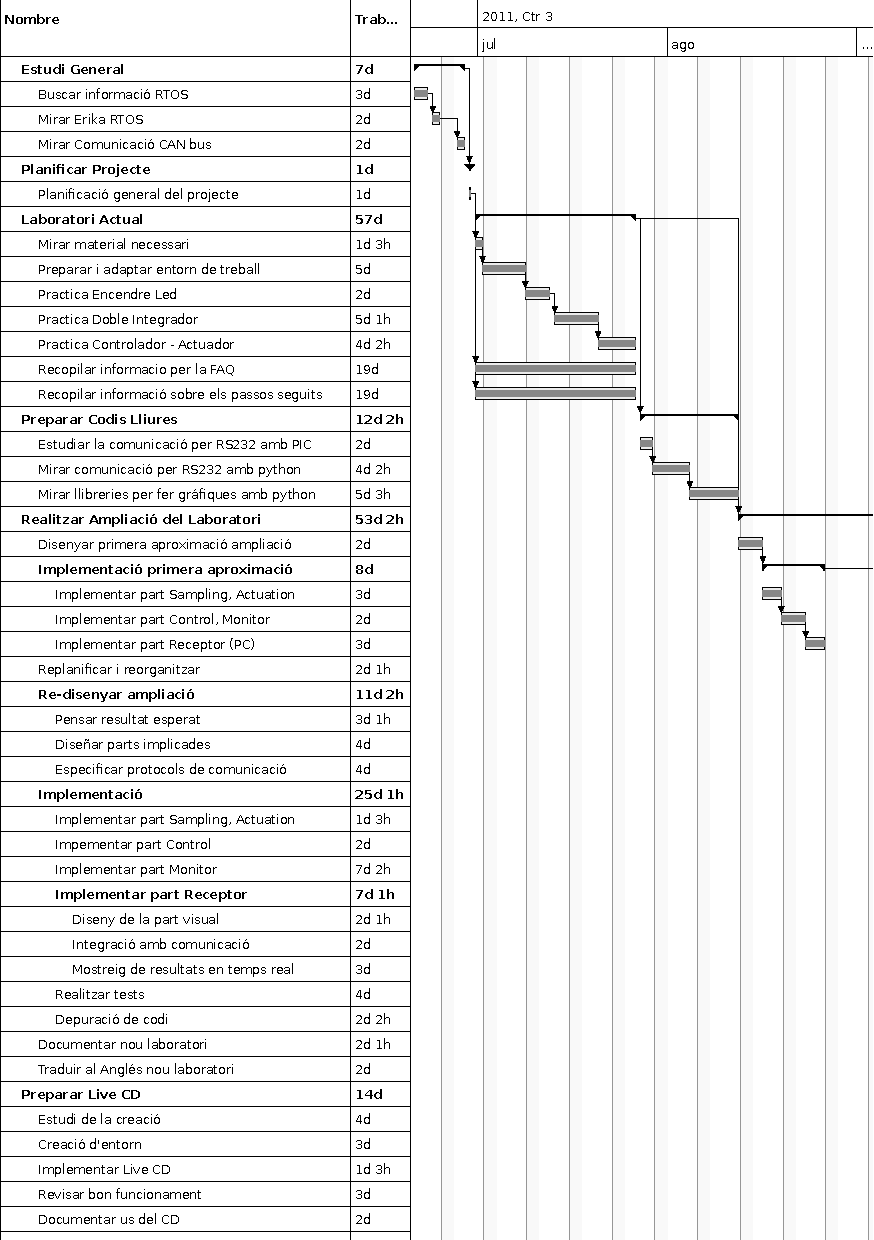
\includegraphics[width=1\textwidth]{gantt_nuevo_v_pag1}
	\end{leftfullpage}
	\caption[Principi del Gantt, esquerre]{\textbf{Principi del Gantt, esquerre} : Juny, Juliol, Agost}
	\label{gantt_nuevo_v_pag1}
\end{figure}
\begin{figure}[p]% will be the right-side figure
	\begin{fullpage}
		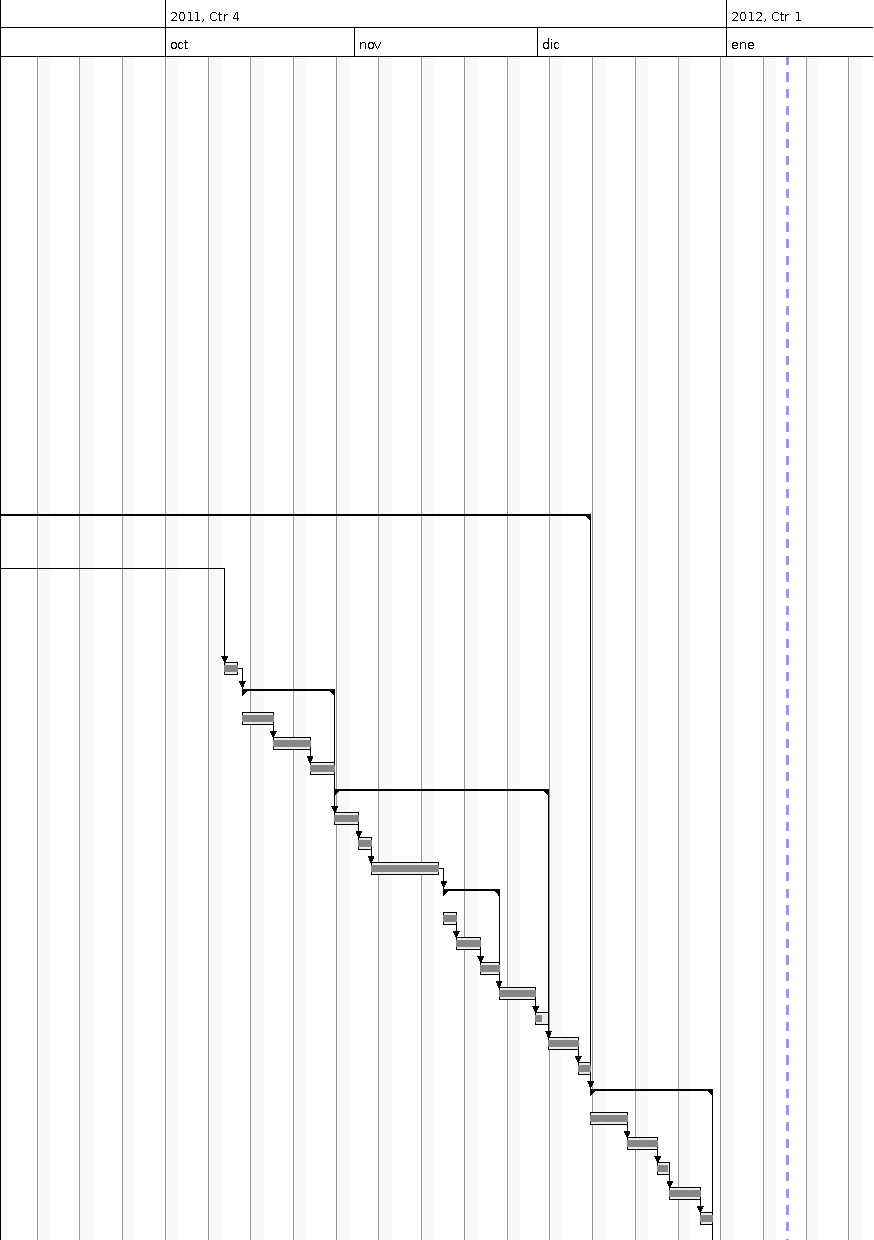
\includegraphics[width=1\textwidth]{gantt_nuevo_v_pag2}
	\end{fullpage}
	\caption[Principi del Gantt, dreta]{\textbf{Principi del Gantt, dreta} : Septembre, Octubre, Novembre, Desembre, Gener}
	\label{gantt_nuevo_v_pag2}
\end{figure}

\begin{figure}[p]% will be the left-side figure
	\begin{leftfullpage}
		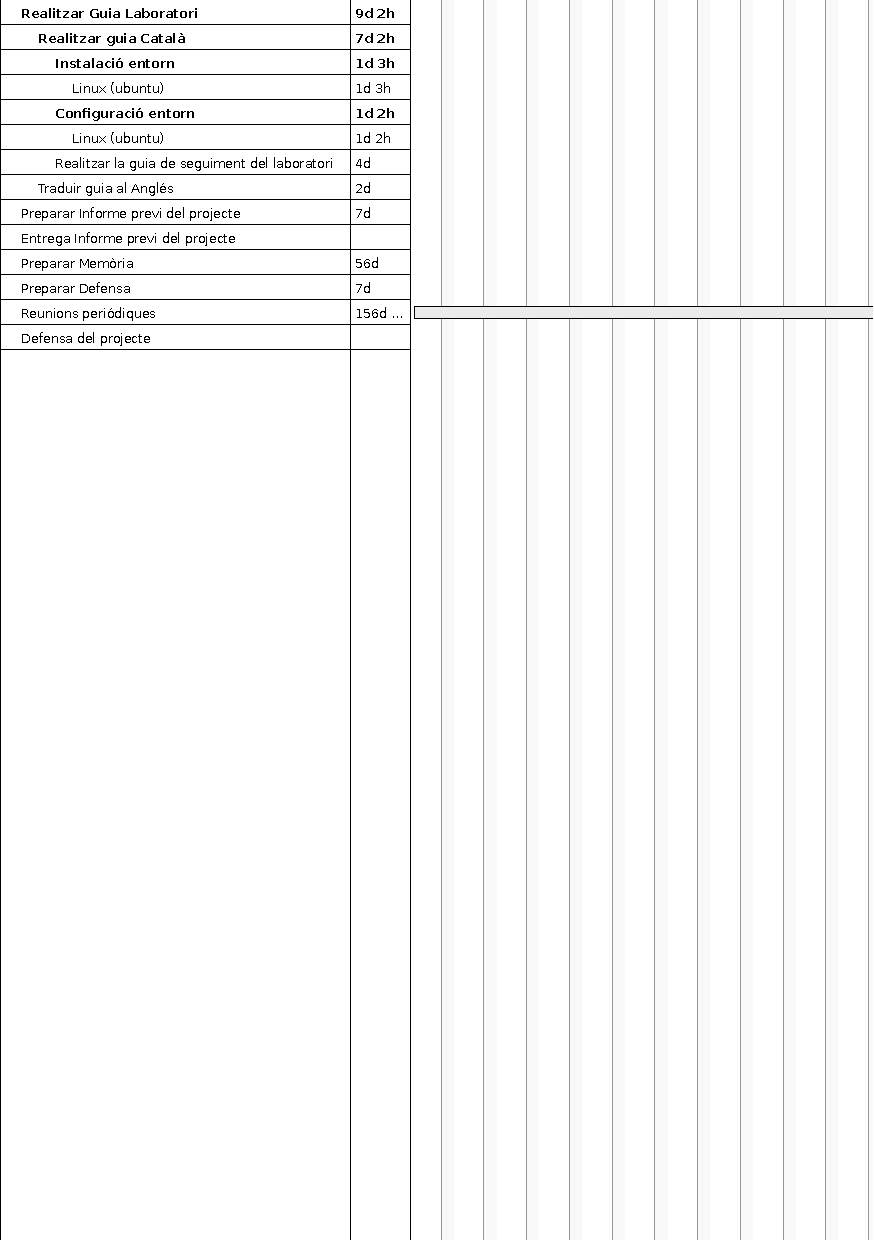
\includegraphics[width=1\textwidth]{gantt_nuevo_v_pag3}
	\end{leftfullpage}
	\caption[Final del Gantt, esquerre]{\textbf{Final del Gantt, esquerre} : Juny, Juliol, Agost}
	\label{gantt_nuevo_v_pag3}
\end{figure}
\begin{figure}[p]% will be the right-side figure
	\begin{fullpage}
		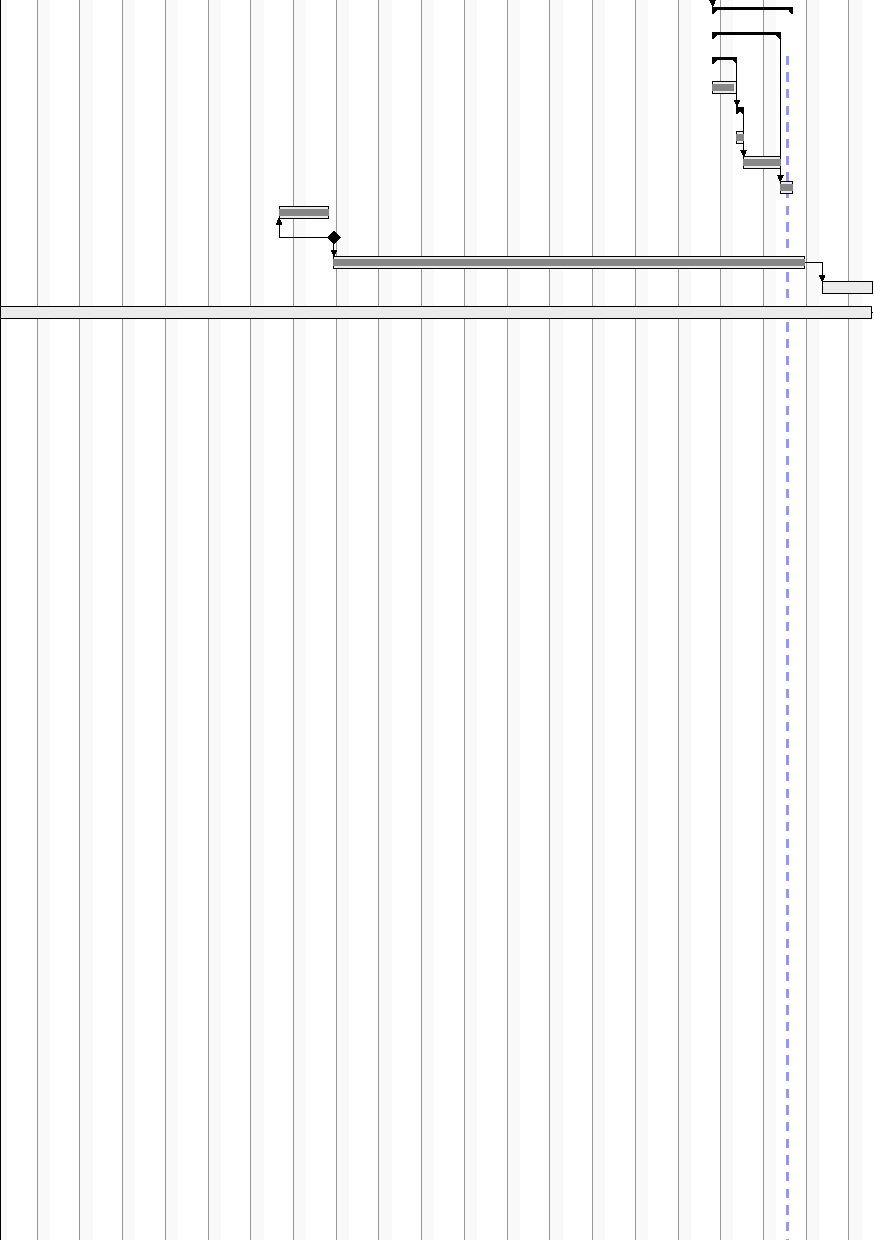
\includegraphics[width=1\textwidth]{gantt_nuevo_v_pag4}
	\end{fullpage}
	\caption[Final del Gantt, dreta]{\textbf{Final del Gantt, dreta} : Septembre, Octubre, Novembre, Desembre, Gener}
	\label{gantt_nuevo_v_pag4}
\end{figure}
  

\clearpage

%: ----------------------- HELP: references
% References can be links to figures, tables, sections, or references.
% For figures, tables, and text you define the target of the link with \label{XYZ}. Then you call cross-link with the command \ref{XYZ}, as above
% Citations are bound in a very similar way with \cite{XYZ}. You store your references in a BibTex file with a programme like BibDesk.


% ----------------------------------------------------------------------



	% background information
% this file is called up by thesis.tex
% content in this file will be fed into the main document

\chapter{Tecnologia}\label{cap:tec} % top level followed by section, subsection

% the code below specifies where the figures are stored
\ifpdf
    \graphicspath{{2_technology/figures/PNG/}{2_technology/figures/PDF/}{2_technology/figures/}}
\else
    \graphicspath{{2_technology/figures/EPS/}{2_technology/figures/}}
\fi

% ----------------------- contents from here ------------------------

Una part molt important del projecte, ha estat familiaritzar-se amb una serie de tecnologies, materials i protocols que en certs casos eren totalment desconeguts. Aquestes tecnologies han comportat hores de dedicació i adaptació i per aquesta mateixa raó s'ha creat aquesta secció. Això permetrà que un lector que no conegui alguna d'aquestes tecnologies pugui de manera rapida fer-se una idea del seu significat o propòsit.

En el capítol Tecnologia per tant s'intentarà donar una visió del tot el material que s'ha usat en el laboratori, per a que serveix cada un dels diferents dispositius i quines característiques tenen (tot això en la secció de Hardware \ref{cap:tec:hard}). 

Tot seguit s'explicarà quins són els programes que es poden utilitzar per compilar els diferents codis, els programes que ens ajuden a programar els dispositius que formen els llaços de control, els programes que ens han permès crear les interfícies, o traduir-les còmodament en el programa \DCSMonitor (tot això en la secció Software \ref{cap:tec:soft}).

I perquè es pugui entendre una mica millor tot el projecte, es dona una visió general sobre els diferents protocols que durant la memòria es veuran, i que han estat necessaris per poder realitzar els controls del laboratori (secció de protocols de comunicació \ref{cap:tec:prot}).

Per tant aquesta secció es fa una eina bàsica necessària per tothom que vulgui comprendre una mica tot això, o per algú que vulgui repassar-ho.

%====================================================================================%
% Hardware
%====================================================================================%
\section{Hardware}\label{cap:tec:hard}

Com hem dit en la introducció d'aquest capítol, en aquesta secció es donarà una visió del material que s'ha utilitzat en l'elaboració del laboratori de Sistemes Distribuïts de Control. Entre aquest material n'hi ha que esta ja preparat per el seu us directe com la placa \FLEX (secció \ref{cap:tec:hard:flex}) i el programador ICD2 (secció \ref{cap:tec:hard:icd}). O en canvi necessita ser ensamblat en un protoboard o crear una placa per poder utilitzar-los. En el nostre cas el microcontrolador dsPIC (secció \ref{cap:tec:hard:dspic}) ja forma part de la placa \FLEX, i per utilitzar el transceptor (secció \ref{cap:tec:hard:mcp2551}), si que s'ha hagut de crear una petita plaqueta que s'explicarà en un altre capítol (secció \ref{cap:dis:resum}).

%====================================================================================%
% FLEX
%====================================================================================%
\subsection{FLEX}\label{cap:tec:hard:flex}

\figuremacroNW{evidence}{Logotip de la companyia Evidence}{}{0.3}

\FLEX és el nom amb el que han designat a una placa de prototipatge creada per la casa Evidence (logotip \ref{evidence}) per treure el màxim partit d'un microcontrolador amb tecnologia dsPIC.

Aquesta placa va néixer amb l'objectiu de desenvolupar aplicacions en temps real, i per aquest motiu compte amb moltes qualitats interessants per el nostre laboratori.

Entre les seves característiques es troben:

\begin{itemize}
	\item Un disseny de la electrònica robust.
	\item Una arquitectura modular.
	\item Disponibilitat d'un gran nombre creixent de guies d'aplicacions.
	\item Tot el suport del kernel Erika Enterprise, de Evidence.
\end{itemize}

El cor d'aquesta placa es composa d'un dsPIC33FJ256MC710 (veure secció \ref{cap:tec:hard:dspic}), el qual ens dona moltes possibilitats a l'hora de crear diferents dispositius.

\figuremacroW{flex_boards}{FLEX: placa de avaluació de dsPIC de \Microchip}{}{0.8}

\clearpage

%====================================================================================%
% dsPIC33FJ256MC710
%====================================================================================%
\subsection{dsPIC33FJ256MC710}\label{cap:tec:hard:dspic}

\figuremacroNW{dspic33fj256mc710}{Fotografia d'un dsPIC33FJ256MC710}{}{0.3}

Aquest és un microcontrolador de la casa \Microchip Technology (fabricant de microcontroladors, memòries i semiconductors analògics, situat en Chandler, Arizona, EE.UU.), destinat a Sistemes Digitals de Control. Per aquesta raó aquest microcontrolador compta amb una multitud de perifèrics de comunicació, entre els quals es troba el CAN. Això fa que la casa Evidence l'hagi escollit per formar part del nucli de la placa de desenvolupament \FLEX (explicada en la secció \ref{cap:tec:hard:flex}), i que s'hagi adaptat el Sistema Operatiu en Temps Real Erika Enterprise perquè pugui ser instal·lat en ell.

A part del mencionat, aquest microcontolador compta amb característiques molt interessants, entre d'elles es poden destacar les següents  (informació extreta del datasheet \cite{DataSheetdsPIC33}):

\begin{itemize}
	\item Una arquitectura de 16 bits
	\item CPU a velocitat de 40 MIPS (Mega Instructions Per Second)
	\item Memòria per programa de 256 KB de tipus Flash
	\item Memòria RAM de 30,720 Bytes
	\item 85 pins d'entrada/sortida
	\item Perifèrics de comunicació UART, SPI, I2C i CAN
	\item PWM amb resolució màxima de 16 bits
	\item 8 canals DMA hardware
\end{itemize}

%====================================================================================%
% MCP2551
%====================================================================================%
\subsection{MCP2551}\label{cap:tec:hard:mcp2551}

\figuremacroNW{mcp2551}{MCP2551}{}{0.3}

El semiconductor MCP2551 és un transceptor CAN d'alta velocitat, i un dispositiu tolerant a fallades que serveix d'intermediari entre el el controlador CAN i el bus físic. Aquest pot arribar a treballar a velocitats de 1 Mb/s, i en un bus CAN es poden arribar a connectar fins a 112 nodes amb aquest transceptor (datasheet \cite{MCP2551}).

Per tant en el nostre laboratori, cada un dels diferents dispositius (\Monitor, \SensorActuador i \Controlador), necessàriament han de comptar amb aquest semiconductor, i s'han creat uns petits circuits per connectar ràpidament en cadascuna de les plaques \FLEX (veure laboratori actual \ref{cap:dis:resum}).

%====================================================================================%
% ICD2/3
%====================================================================================%
\subsection{ICD2/3}\label{cap:tec:hard:icd}

\figuremacroNW{icd2}{Fotografia d'un programador ICD2}{}{0.3}

Aquest aparell (figura \ref{icd2}) és un programador/debugador d'errors, fabricat per la casa \Microchip, que juntament amb el programa \MplabX pot realitzar aquestes funcions. Aquest compta amb una connexió per USB per connectar-lo al ordinador, i un cable amb dos extrems RJ-11 per connectar entre ell i el dispositiu a programar (figura \ref{RJ11}, connector típicament utilitzat en els cables telefònics a España).

Mentre que fins aquest moment s'utilitzava el programador ICD2 actualment ha sortit al mercat el ICD3. Això en principi no és cap problema ja que l'antic programador segueix funcionant correctament, però així com el programa \MplabX en les primeres versions betes estava procurant donar suport al primer, a partir de la versió 0.17 ha deixat de ser així, obligant d'alguna manera a deixar enrere aquest programadors; els quals no són precisament barats.

\figuremacroW{RJ11}{Connector RJ-11}{}{0.3}

\FloatBarrier

%====================================================================================%
% Software
%====================================================================================%
\section{Software}\label{cap:tec:soft}

Durant el projecte s'han emprat multitud de programes que eren necessaris per poder compilar els codis, gravar els microcontroladors, o preparar l'entorn multilingüe del programa \DCSMonitor.

En aquesta secció s'explicarà quins són aquests programes, i es farà un resum del seu objectiu.

%====================================================================================%
% Eclipse
%====================================================================================%
\subsection{Eclipse}\label{cap:tec:soft:eclipse}

\figuremacroNW{eclipse_2}{Logotip d'Eclipse}{}{0.3}

Aquest software ens ofereix un entorn de desenvolupament integrat (també coneguts com IDE's) multiplataforma de codi obert. Aquesta plataforma ha estat típicament utilitzada per desenvolupar IDE's. Típicament és usat el IDE de Java \emph{Java Development toolkit} (JDT) el qual ve integrat per defecte amb el propi \Eclipse.

Entre aquests IDE's desenvolupats per \Eclipse està el RT-Druid (figura \ref{rt_druid}) creat per la casa Evidence, amb el qual és possible programar de manera facil el Sistema Operatiu en Temps Real Erika, que és el codi base sobre el que treballem en el laboratori per programar les plaques \FLEX.

A part d'utilitzar aquest IDE per programar els dispositius, també existeix el pluguin PyDev per \Eclipse, que també ens ofereix un IDE per programar en \Python, i gracies al qual hem pogut programar més facilment el codi del programa \DCSMonitor.
\figuremacroW{rt_druid}{Logotip del pluguin d'\Eclipse RT-Druid}{}{0.4}

\figuremacroW{pydev}{Logotip del pluguin d'\Eclipse PyDev}{}{0.4}

%\FloatBarrier

%====================================================================================%
% Mplab
%====================================================================================%
\subsection{\MplabX}\label{cap:tec:soft:mplab}


Mplab és un editor IDE gratuït desenvolupat per la casa Microchip i destinat a la programació dels seus productes. Fins aquest moment era exclusivament per Windows, però amb la nova aparició de \MplabX programat en Java l'han convertit en multiplataforma. Encara que les versions actuals encara estan en beta (això vol dir que algunes de les seves funcionalitats encara poden ser inestables o no estar implementades).

\figuremacroW{mplabx}{Logotip de \MplabX}{Publicitat de la pàgina oficial de Microchip}{0.7}

Encara que sigui un editor IDE, en el nostre laboratori no l'utilitzem per aquesta tasca, ja que això ens ho fa l'entorn comentat anteriorment RT-Druid (veure secció d'Eclipse \ref{cap:tec:soft:eclipse}). Per tant te una altra funcionalitat que és la de programar mitjançant el dispositiu ICD2 o altres els microcontroladors; en el nostre cas les plaques \FLEX.


%====================================================================================%
% QtCreator
%====================================================================================%
\subsection{QtCreator}\label{cap:tec:soft:qtcreator}

\figuremacroNW{qtcreator}{Logotip de QtCreator}{}{0.3}

QtCreator és un altre IDE per desenvolupar aplicacions d'escriptori multiplataforma (tant el programa com les interfícies que és capaç de generar poden ser executats en Windows, Linux/X11 i Mac OS). Aquesta eina ens ha sigut molt útil a l'hora de dissenyar tota la part visual del programa \DCSMonitor, ja que l'entorn que proporciona aquest programa és molt senzill d'utilitzar, i ofereix un gran ventall de possibilitats, com poden ser els botons, les etiquetes, els menús, la finestra de exportar les gràfiques, la integració amb les gràfiques en temps real, etc.

Encara que té moltes característiques interessants nosaltres només l'hem utilitzat per fer l'entorn gràfic en un fitxer de format .ui, per després exportar-lo per Python.

%====================================================================================%
% QtLingüist
%====================================================================================%
\subsection{QtLingüist}\label{cap:tec:soft:qtlinguist}

%\figuremacroNW{qt-linguist}{Logotip de QtLingüist}{}{0.2}

\begin{wrapfigure}{r}{0.3\textwidth}
	\centering
	
\includegraphics[width=0.27\textwidth]{qt-linguist}
	\caption[Logotip de QtLingüist]{{\small\textbf{Logotip de QtLingüist}}}
	\label{qt-linguist}
\end{wrapfigure}

Qt ens ofereix suport per traduir les aplicacions en altres llenguatges, i gracies a aquest programa podem editar els fitxers de traducció fàcilment, i un cop traduïts tots els textos, el mateix \Qtlinguist ens genera el fitxer adequat perquè el nostre programa \DCSMonitor pugui canviar l'idioma en qualsevol moment.

%====================================================================================%
% ERIKA Enterprise
%====================================================================================%
\subsection{ERIKA Enterprise}\label{cap:tec:soft:erika}

\figuremacroN{erika_enterprise}{Logotip Erika Enterprise}{}

ERIKA Enterprise \ref{erika_enterprise} és un Sistema Operatiu en Temps Real de codi obert derivat de OSEK/VDX (veure glossari), creat per la casa Evidence i que està integrat en el plugin RT-Druid d'Eclipse.

Erika ens ofereix un RTOS d'espai reduït (1-4 Kb Flash) per sistemes empotrats d'un sol nucli o multi-nucli.

Aquest sistema operatiu és usat actualment en més de 20 universitats de tot el mon, a més de varies companyies del mercat automobilístic (entre d'elles Magneti Marelli Powertrain i Cobra Automotive Technologies).


%====================================================================================%
% Protocols de comunicació
%====================================================================================%
\section{Protocols de comunicació}\label{cap:tec:prot}

Les comunicacions en els Sistemes Distribuïts de Control són el pilar mestre sobre el que es recolza el control, per aquesta raó la major part del projecte es bassa en aquestes qüestions, i es dissenyen els diferents missatges i identificadors de manera que es pugui maximitzar l'us dels avantatges que té cada protocol. 

En aquesta secció es podrà veure un repas general sobre el tipus de protocols usats en el laboratori, així com el tipus de connexionat que existeix entre els diferents dispositius que el formen.

%====================================================================================%
% CAN
%====================================================================================%
\subsection{CAN}\label{cap:tec:prot:can}

El protocol CAN (de l'Anglès Controller Area Network) va ser dissenyat per permetre la comunicació entre dispositius sense la necessitat d'un host (o amfitrió). Inicialment la seva aparició va esdevenir de la problemàtica que existia en els vehicles automòbils, en els quals el nombre de dispositius era cada cop més gran, fins arribar al punt de necessitar més de 2 km de cable, els quals representaven més de 100 Kg (informació extreta de \cite{ComIndCAN}, \cite{CapaFisicaCAN}).

Va ser la firma Alemana \emph{Robert Bosch GmbH} , qui va desenvolupar aquest protocol, basat en una topologia bus per la transmissió de missatges en entorns distribuïts, inicialment (com hem dit anteriorment) per l'entorn automobilístic, però finalment acollit per entorns marins, agrícoles, industrials, etc.

Les característiques més importants de la comunicació CAN són les següents (especificació,  \cite{Bosch1991}):

\begin{itemize}
	\item Jerarquia de nodes multimaster.
	\item Tècnica d'accés al medi CSMA/CD+CR (de l'anglès Carrier Sense, Multiple Access/Collision Detection + Collision Resolution).
	\item Comunicació conduïda per events.
	\item Broadcast.
	\item Iniciativa de transmissió a càrrec de la font d'informació.
	\item El nom del missatge genèricament dessigna la informació, no el node.
	\item Resposta a petició remota.
	\item Detecció i correcció d'error a nivell de missatge.
	\item Capacitat de detecció d'errors a nivell del medi de comunicació.
	\item Tolerància a fallades.
	\item Confirmació.
	\item Transferència de missatges consistent sobre tot el sistema.
	\item Codificació de bit.
	\item Sincronització de bit.
	\item Sincronització entre nodes.
	\item Distribució del sistema.
	\item Velocitat de transmissió.
	\item Característiques del driver de línia.
	\item Múltiples proveïdors de xips.
\end{itemize}

%====================================================================================%
% Serie RS232
%====================================================================================%
\subsection{Serie via RS232}\label{cap:tec:prot:rs232}

En computació la comunicació serie és tota aquella transferència de dades en la que la informació va bit a bit una darrera una altra. Aquest tipus de comunicació és usada en multiples protocols de comunicació, com poden ser el USB, Ethernet, FireWire o per exemple CAN (vist anteriorment \ref{cap:tec:prot:can}). Però usualment, quan parlem del port serie de l'ordinador, ens referim a la norma RS232 (de l'anglès Recommended Standard 232) (veure \cite{Wikipedia2012}).

Aquesta norma determina les seves característiques físiques, la temporització dels senyals, les velocitats de transmissió, i la mida del connector i dels seu pinatge.

\figuremacroN{SerialPort_ATX}{Connector per port serie RS232}{En forma de DE-9}

Normalment tots els ordinadors de sobretaula solen tenir algun connector destinat a aquest tipus de comunicació, en el format d'un connector DB-9 (originalment DE-9, veure figura \ref{SerialPort_ATX}), en canvi els ordinadors portàtils ja no solen tenir aquest tipus de connector, per aquesta raó es necessita utilitzar un convertidor de RS232 a USB.

Aquesta comunicació va ser dissenyada per connectar equips terminals de dades amb equips de comunicació de dades, però en ocasions (com en el cas del connexionat entre dos ordinadors) es connecten dues terminals de dades. En aquest cas es sol utilitzar un tipus de connexionat anomena null módem (per la no existència de módem).

El connector DB-9; com el seu nom indica; té 9 pins, i cada un d'ells te definit el seu funcionament, com pot ser el d'enviar dades, o el de rebre dades. S'adjunta una taula amb l'especificació de cada un d'aquests pins (taula tab:tec:prot:rs232).

\begin{table}[ht!]
	\begin{center}
	\begin{tabular}{ | c | l | }
\hline
Número de pin	&Nom\\
\hline
1	&CD: Detector de transmissió\\
\hline
2	&RXD: Recepció de dades\\
\hline
3	&TXD: Transmissió de dades\\
\hline
4	&DTR: Terminal de dades preparat\\
\hline
5	&GND: Senyal de terra\\
\hline
6	&DSR: Ajust de dades preparat\\
\hline
7	&RTS: Permís per transmetre\\
\hline
8	&CTS: Preparat per transmetre\\
\hline
9	&RI: Indicador de trucada\\
\hline
	\end{tabular}
	\end {center}
	\captionof{table}{Pinatge del connector serie per RS232}
	\label{tab:tec:prot:rs232}
\end{table}


%====================================================================================%
% Topologia en bus
%====================================================================================%
\subsection{Topologia en bus}\label{cap:tec:prot:bus}

Aquest és un tipus de connexionat entre múltiples dispositius en els quals tots ells estan connectats a un mateix bus central (veure figura \ref{Bus_Topology}). Això comporta alguns avantatges però també molts inconvenients que es procuren resoldre de diferents maneres.

Per crear aquest tipus de xarxa és necessari finalitzar els cables amb resistències de carrega final. Aquestes resistències són calculades depenent de les senyals que hi circulen, i els metres de cable que formen el bus, i aconsegueixen mitigar l'efecte rebot que apareix en un cable tallat (amb la resistència ben calculada a ulls dels dispositius el bus resultaria ser de mida infinita).

\begin{itemize}
	\item Avantatges
		\begin{itemize}
			\item Facilitat en la implementació.
			\item Creixement del nombre de dispositius fàcil.
			\item Simplicitat en el tipus d'arquitectura.
			\item Recepció de tota la informació del bus.
			\item No hi ha necessitat de redireccionar missatges.
		\end{itemize}
	\item Inconvenients
		\begin{itemize}
			\item Existeix un  límit del nombre de dispositius, depenent de la qualitat del senyal.
			\item Pot produir-se degradació del senyal.
			\item Complexitat de reconfiguració i aïllament de fallades.
			\item Un problema en un canal sol degradar tot el bus.
			\item El bon funcionament sol degradar a mesura que el bus creix.
			\item El bus ha de ser degudament tancat.
			\item Alta pèrdua de transmissions degut a les col·lisions entre missatges.
		\end{itemize}
\end{itemize}

\figuremacroW{Bus_Topology}{Topologia en bus}{}{0.5}

\FloatBarrier

%====================================================================================%
% Conclusions
%====================================================================================%
\section{Conclusions}\label{cap:tec:conc}

En aquest punt ja ens hem fet una idea de totes les tecnologies que hi ha al voltant d'aquest projecte. Hem vist que les xarxes en bus tenen alguns inconvenients que cal resoldre, quines facilitats ens proporciona utilitzar un bus CAN, com podem rebre els valors d'estat del control mitjançant la comunicació serie via RS232, i quins dispositius s'utilitzen per poder connectar-se a un bus CAN, anomenats transceptor CAN.

També hem pogut conèixer varis programes que ens ajuden en la tasca de programar tots aquests dispositius, com crear interfícies per programes que corrin en varis sistemes operatius, i com generar aquests programes multilingües.

Per tant ja podem abordar la configuració que té el laboratori actual, i podem començar a dissenyar tot el necessari per muntar un laboratori en el que tots els dispositius comparteixin un mateix bus CAN. Tot això ho podrem veure i seguir en el següent capítol.
		% aims of the project

%%==================================================================%%
%% Author : Perelló Nieto, Miquel                                   %%
%% Version: 1.0, 04/11/2011                                         %%
%%                                                                  %%
%% Memoria del Projecte de Final de Carrera                         %%
%% Disseny del laboratori                                           %%
%%==================================================================%%

\chapter{Disseny del laboratori}\label{cap:dis}


% the code below specifies where the figures are stored
\ifpdf
    \graphicspath{{3_laboratory_design/figures/PNG/}{3_laboratory_design/figures/PDF/}{3_laboratory_design/figures/}}
\else
    \graphicspath{{3_laboratory_design/figures/EPS/}{3_laboratory_design/figures/}}
\fi


% ----------------------- contents from here ------------------------

Aquest capítol comença amb l'explicació de l'entorn i dels objectius que té el laboratori actual de Sistemes de Control Empotrats i en Xarxa. Exposarem per tant el seu proposit i les limitacions que aquest tenía, i de quina manera hem dissenyat la nova plataforma per poder solventar algunes d'aquestes mancanses.
Per tant entrarem en la part del disseny del nou laboratori, i veurem les raons que ens han portat a escollir els diferents camins que teniem, així com el disseny de les comunicacions que hi ha entre els diferents dispositius i el nou programa \DCSMonitor.

%====================================================================================%
% Laboratori actual
%====================================================================================%
\section{Resum del laboratori actual}\label{cap:dis:resum}

L'objectiu d'aquest laboratori és l'analisis, el diseny i la implementació d'un sistema de control empotrat i en xarxa (a partir d'ara \NECS, sigles de l'anglès Networked and Embedded Control Systems) \cite[laboratori complert en el document \emph{Networked and Embedded Control Systems (NECS) Double Integrator Control Lab}]{NECSDoubInt}.

En aquest laboratori es cobreixen varies fases:

\begin{itemize}
	\item Disseny de controls.
	\item Anàlisis de sistemes \NECS multitasques.
	\item Diseny de sistemes \NECS multitasques.
	\item Implementació del sistema \NECS.
\end{itemize}

La plataforma d'implementació ens permetrà controlar un circuit Doble Integrador (a partir d'ara \DI de l'anglés Double Integrator) d'un microcontrolador. Com es mostra en les figures \ref{microprocessor_based_control} i \ref{network_based_control}.

\figuremacroW{microprocessor_based_control}{Microprecessor-based control}{}{0.35}

\figuremacroW{network_based_control}{Network-based control}{}{0.6}

En la primera configuració, figura \ref{microprocessor_based_control}, moltes tasques són executades concurrentment al cap davant del Sistema Operatiu en Temps Real Erika. Per aquesta raó les tasques de control del circuit doble integrador han de competir amb la resta per el temps de CPU.

En la segona configuració, figura \ref{network_based_control}, permet tancar el llaç de control en una xarxa, en aquest cas un bus CAN. En aquest escenari, les limitacions dels recursos ve donada per l'ampla de banda de la comunicació. D'aquesta manera connectant varis llaços en una mateixa xarxa ens pot permetre analitzar un sistema distribuït de control més realista.

En les dues configuracions, les plaques estan equipades amb microcontroladors dsPIC33FJ256MC710 de \Microchip. Les plaques són plaques \FLEX de Evidence. S'han creat tres plaques amb un circuit doble integrador (figura \ref{DI_down}), comunicació CAN (figura \ref{DI_up})i un port RS232 (figura \ref{RS232_up}) que s'han afegit a aquestes per tal de comunicar-se entre elles, i amb l'ordinador.

\begin{figure}[ht!]
	\begin{center}
		\subfloat[Doble Integrador]{\label{DI_down}
			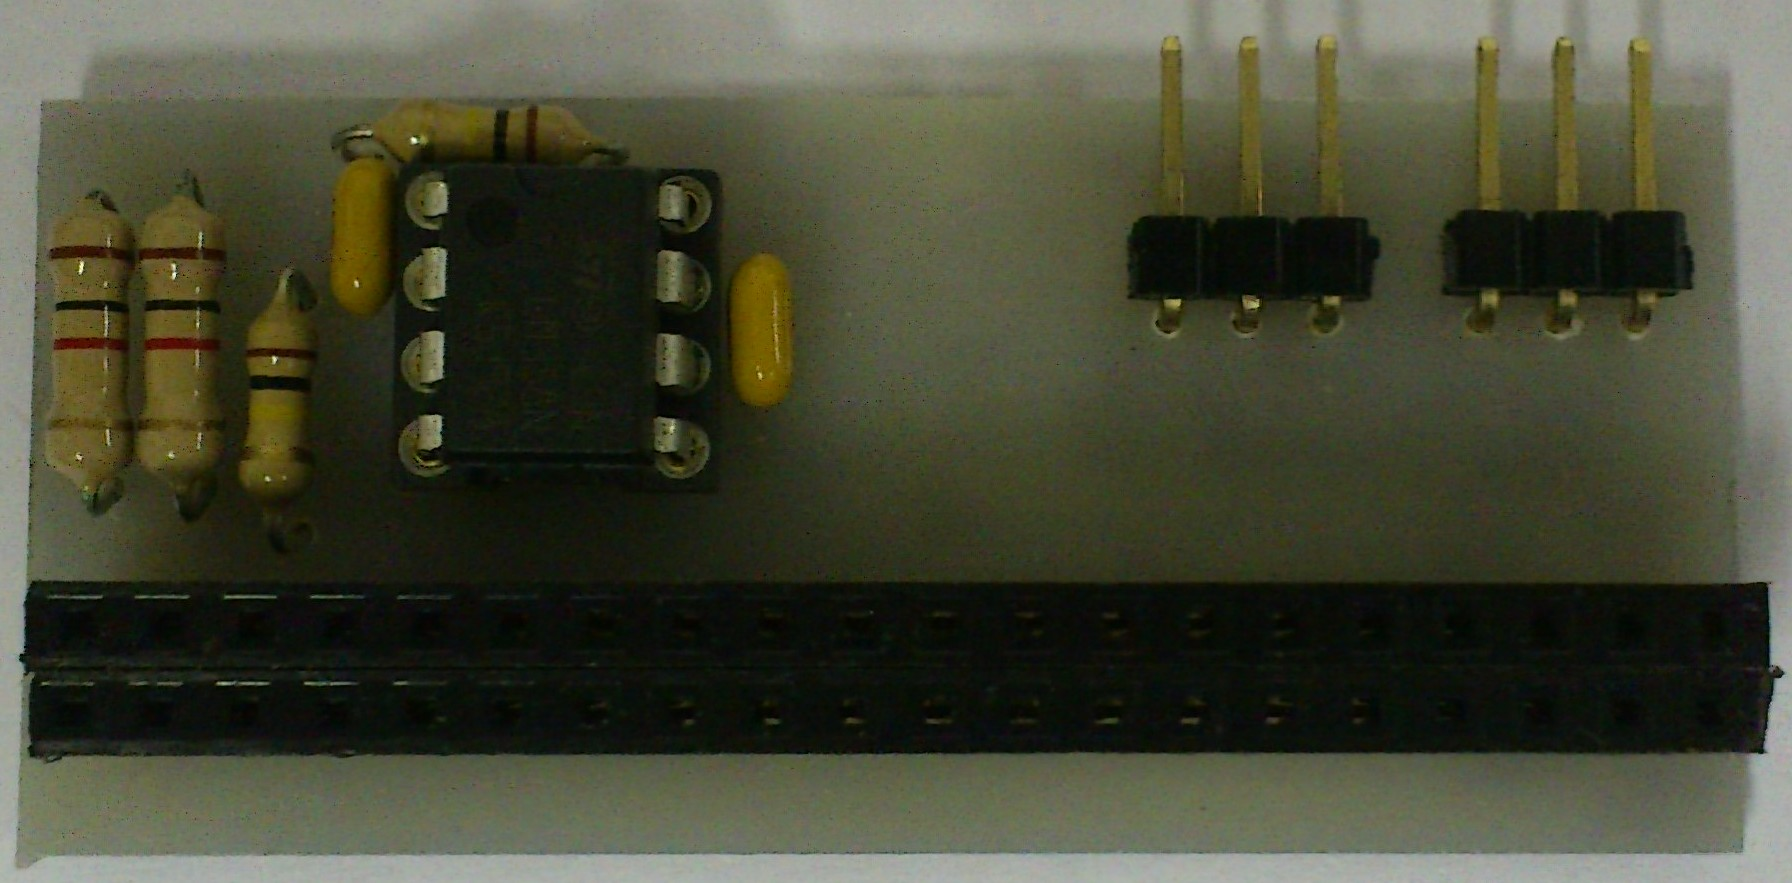
\includegraphics[width=0.4\textwidth]{DI_down}
		}
		\subfloat[Transceptor CAN]{\label{DI_up}
			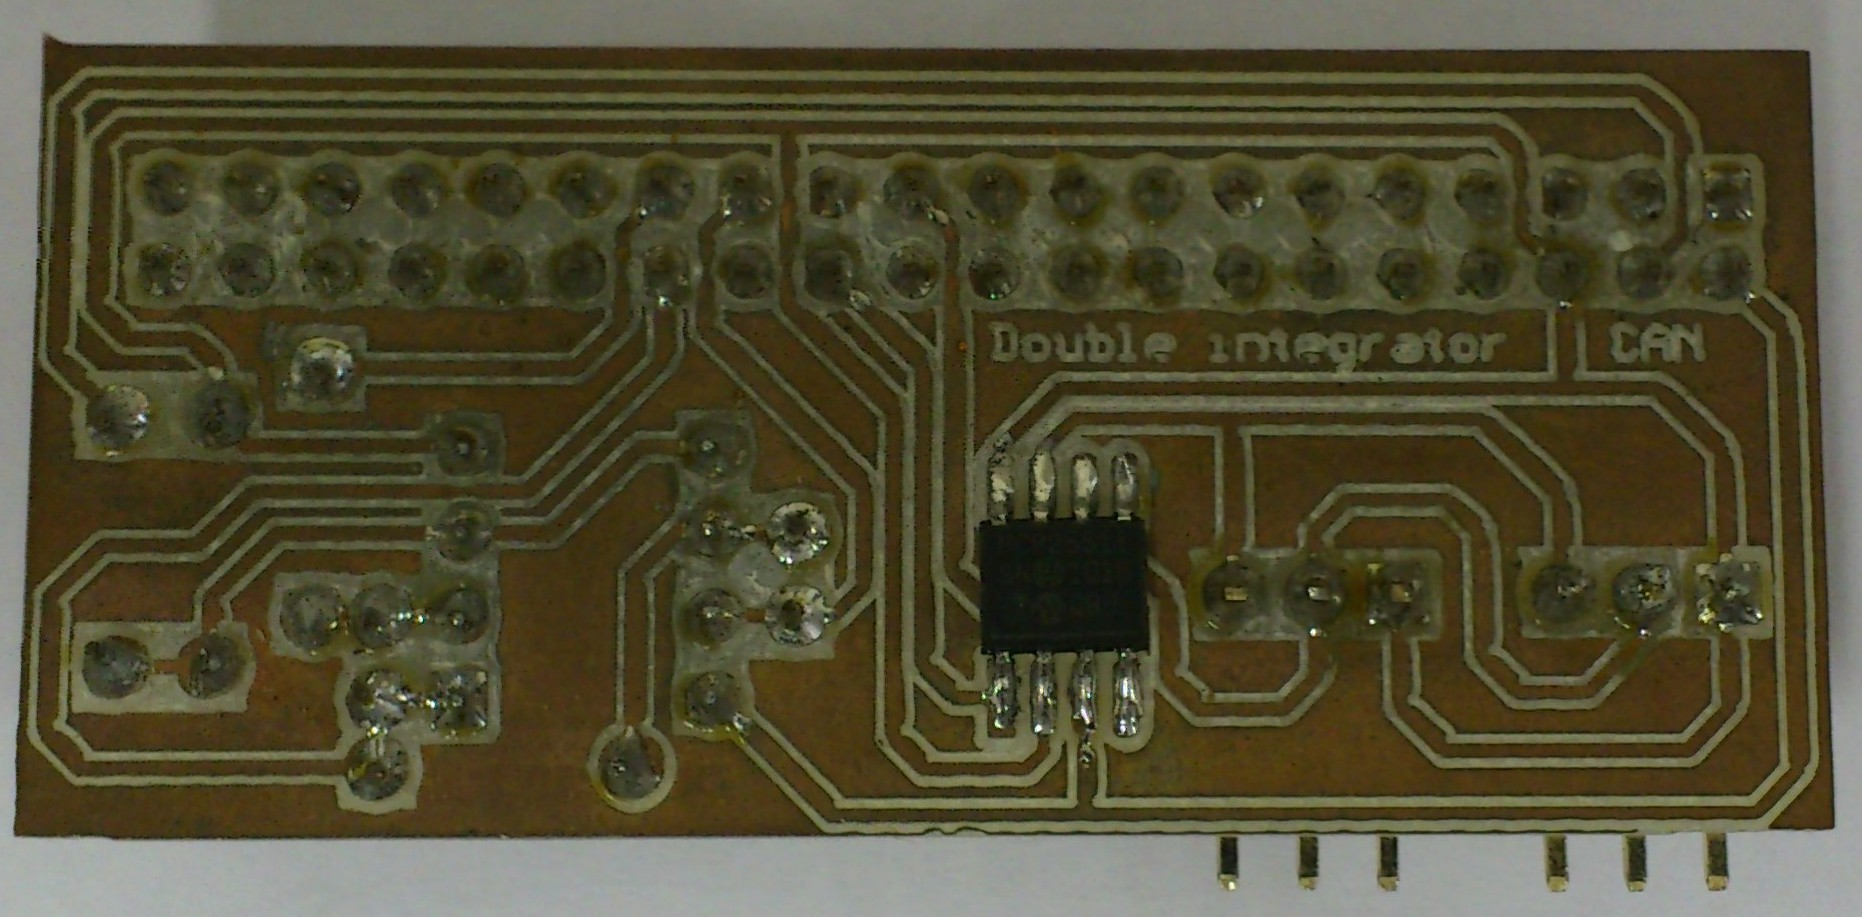
\includegraphics[width=0.4\textwidth]{DI_up}
		}

		\subfloat[Modul RS232]{\label{RS232_up}
			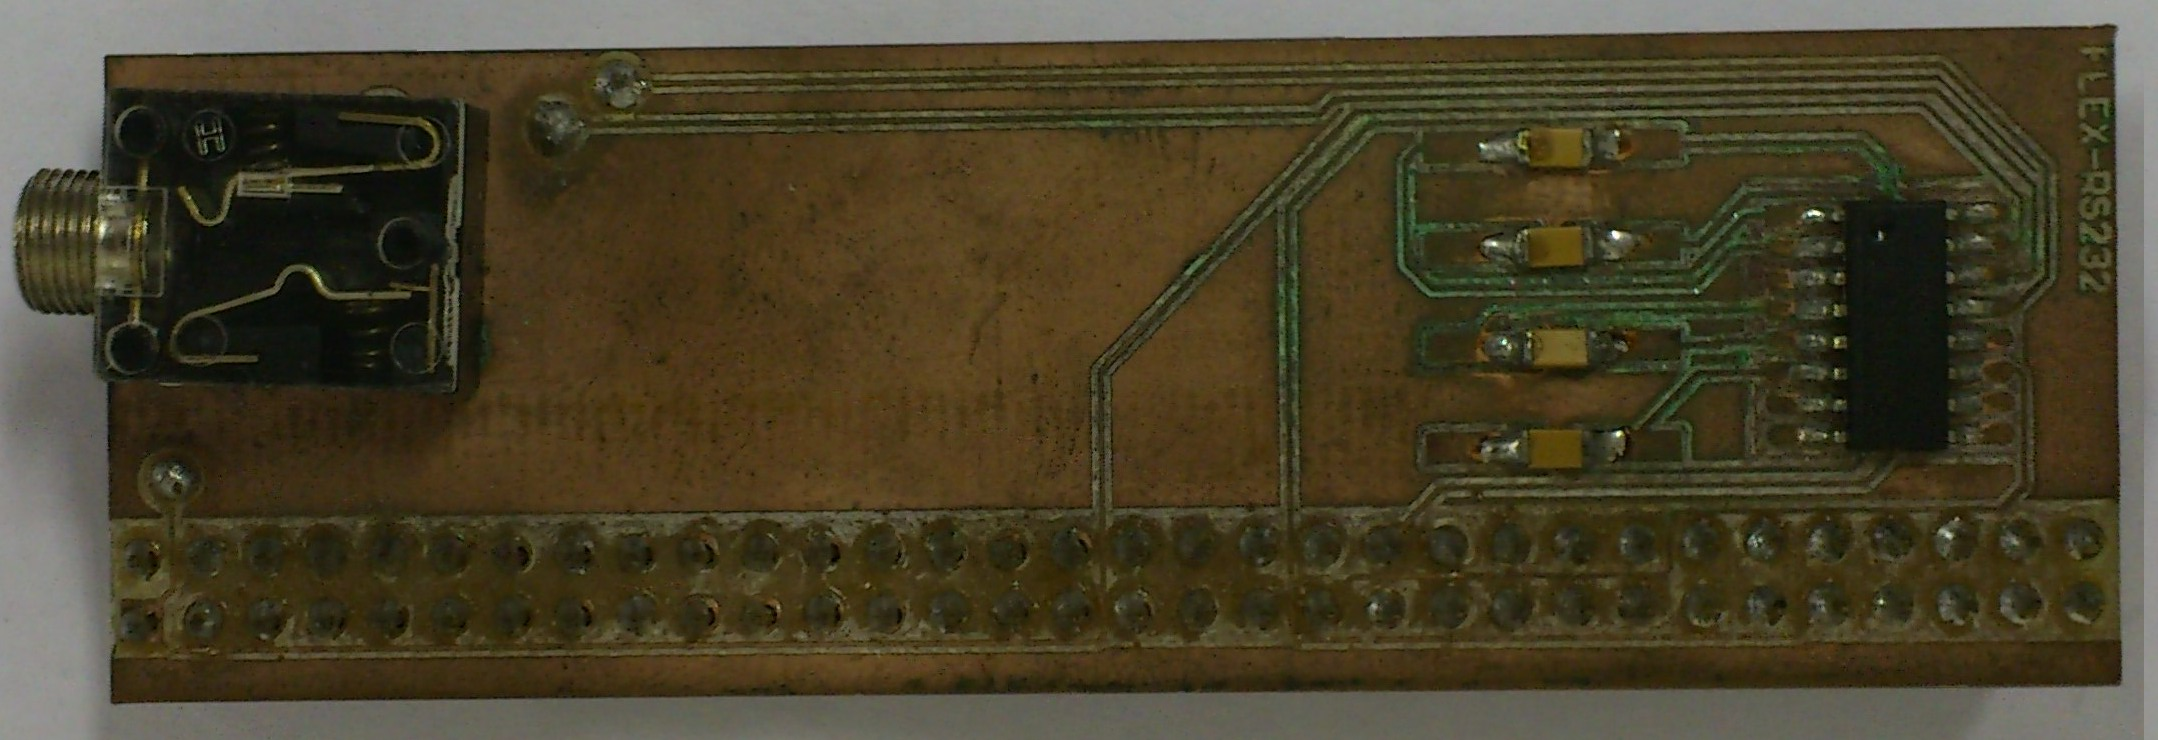
\includegraphics[width=0.6\textwidth]{RS232_up}
		}
	\end{center}
	\caption{Periferics per les plaques \FLEX.}
    \label{fig:plaques}
\end{figure}

La placa \FLEX que porta el circuit doble integrador es l'encarregada de simular un \Sensor i un \Actuador, en els quals el \Sensor es un conversor analogic digital (ADC) que llegeix els voltatges de sortida de la primera i segona integral, i l'\Actuador aplica diferents nivells de voltatge a l'entrada del circuit a través d'un modulador per amplada de polsos (PWM).

L'objectiu del control es que la sortida del doble integrador segueixi un valor de referencia que va variant. Aquest s'aconsegueix aplicant un algoritme de control i aplicant el valor calculat a l'entrada del circuit.

Un cop l'entorn està preparat la configuració queda com a la figura \ref{DCS_NECS_SCA_diagonal}. En la qual la placa superior actua com a \Controlador que remotament fa el control a traves del bus CAN. En la part inferior tenim el \SensorActuador que compta amb la placa del doble integrador connectada, i per tal de debugar el control també compta amb la interfície RS232 (en aquesta imatge queda sota de la placa superior) la qual envia periòdicament els valors de l'estat.


\figuremacroW{DCS_NECS_SCA_diagonal}{Llaç de control}{}{0.5}

\FloatBarrier

%====================================================================================%
% Nou laboratori
%====================================================================================%
\section{Disseny del Nou laboratori}\label{diss:nou}

Fins aquest moment els problemes a resoldre han estat pels temps de demora que hi havia entre lectures del \Sensor, accions de l'\Actuador i els càlculs que havia de fer el \Controlador.

En aquest apartat ens interessa que tots els dispositius estiguin en un mateix bus CAN i comprovar el funcionament dels llaços en un entorn compartit, amb diferents tipus de prioritats i amb la possibilitat de saturar el bus en certes ocasions (figura \ref{DCS_NECS_two_links}).

A part d'aquesta connexió general al bus, també s'introduirà en la xarxa un dispositiu que anomenarem \Monitor, el qual tindrà la opció de monitoritzar tots els paquets de dades d'un cert llaç de control (un grup format per un \Sensor, un \Actuador i un \Controlador).

Tota la informació que el nou dispositiu \Monitor capturi, podrà ser enviada mitjançant el port sèrie RS232 a un programa d'ordinador (\DCSMonitor) el qual mostrarà mitjançant unes gràfiques en temps real l'estat del control de cada grup del laboratori.

A més el \Monitor tindrà la capacitat d'incrementar la carrega del bus en quant a nombre de missatges CAN que hi circulin, dificultant el correcte funcionament dels llaços, i podent comprovar en temps real la resposta d'aquests.

Amb aquesta idea general i tenint en compte les relacions que hi haurà entre tots els elements que formen el laboratori es va dissenyar un esquema general en el que apareixen aquests elements i el tipus de comunicació que hi ha entre ells (figura \ref{esquema_general_v8}).

\figuremacro{DCS_NECS_two_links}{Entorn del nou laboratori}{A l'esquerra un llaç de control format per un \Controlador (primer pis) i un \SensorActuador (segon pis). A la dreta un llaç de control format per un \Controlador (segon pis) i un \SensorActuador (tercer pis) i un dispositiu \Monitor (primer pis).}

% El diagrama de comunicacions ocupa una pagina sencera, i està posicionat horitzontalment, amb aquest ifthenelse el diagrama sempre es mirarà desde la part exterior del llibre, rotant el diagrama 180 graus si cal.
%\ifthenelse {\isodd{\thepage}}
%{
%\figuremacroWR{esquema_general_v8}{Diagrama general dels elements del laboratori}{Diagrama de tots els elements que formen part del laboratori, i les diferents comunicacions que els relacionen.}{1}{180}
%}
%{
%\figuremacroW{esquema_general_v8}{Diagrama general dels elements del laboratori}{Diagrama de tots els elements que formen part del laboratori, i les diferents comunicacions que els relacionen.}{1}
%}

\begin{landscape}
\figuremacroWR{esquema_general_v8}{Diagrama general dels elements del laboratori}{Diagrama de tots els elements que formen part del laboratori, i les diferents comunicacions que els relacionen.}{1}{270}
\end{landscape}
%\figuremacroW{comunicacio_pc_monitor_v6}{Diagrama de comunicacions i identificadors}{Diagrama de funcionament del laboratori, disseny dels identificadors i màscares per bus CAN, i tipus de missatges de comunicació.}{1}

%====================================================================================%
% Interficie
%====================================================================================%
\subsection{Interficie}\label{cap:dis:visual}

Aquest programa es només una eina per visualitzar i comprovar el funcionament dels diferents controls que hi hagin al bus CAN, o el control del llaç al que estigui connectat, però en cap moment ha de ser un programa complicat d'executar, ja que el seu objectiu principal es precisament ajudar en aquesta tasca. Això implicava que el programa fos senzill d'utilitzar, però a l'hora complert.

Primer de tot calia saber quines opcions havien d'aparèixer a primera vista, així que es va fer un llistat d'elements necessaris:

\begin{itemize}
	\item Llista dels identificadors dels diferents controls al bus CAN
	\item Estat del port sèrie RS232
	\item Lectures dels valors del control en format text
	\item Gràfica del control
	\item Mostrar/eliminar dades de la gràfica
		\begin{itemize}
			\item Referència
			\item Valor d'entrada
			\item Primera integral
			\item Segona integral
		\end{itemize}
	\item Idioma per seleccionar
		\begin{itemize}
			\item Català
			\item Espanyol
			\item Anglès
			\item Francès
		\end{itemize}
	\item Mode de comunicació
		\begin{itemize}
			\item Comunicant amb \SensorActuador
			\item Comunicant amb \Monitor
		\end{itemize}
	\item Dades informatives (extres)
		\begin{itemize}
			\item Total de llaços de control al bus CAN
			\item Imatges per segon mostrades en la gràfica en temps real
			\item Nombre de mostres de cada línia de la gràfica
			\item Bytes pendents en el buffer d'entrada del port sèrie RS232
			\item Algun ítem intermitent que indiqui que les dades s'actualitzen correctament (en temps real)
		\end{itemize}
	\item Botó per connectar al port sèrie
	\item Botó per llistar llaços del bus CAN
	\item Botó per guardar una imatge de la gràfica
	\item Botó per netejar el text
	\item Botó per començar i aturar la monitorització
\end{itemize}

Un cop remarcats aquests elements, només calia identificar aquells que havien de ser accessibles directament, i posicionar-los de tal manera que fos intuïtiu d'utilitzar. Per tant es va treure la selecció d'idioma i de mode d'execució de la pantalla principal i es va posar en les \emph{Preferències} del programa, de la mateixa manera amb el mode d'execució del programa ja que els alumnes sempre faran servir el mode \SensorActuador i el professor el mode \Monitor.

Abans de començar a dissenyar la interfície amb algun programa d'edició, es van fer alguns esbossos de com hauria de quedar la organització, i finalment es va decantar pel dibuix de la figura \ref{esquema_interficie}.

\begin{landscape}
\figuremacroWR{esquema_interficie}{Esquema de la interfície del programa \DCSMonitor}{}{1}{270}
\end{landscape}

Ja amb l'esquema ben clar es van provar varis IDE's d'edició d'interfície, i un cop analitzades varies qüestions es va decidir utilitzar \QTCreator. Aquestes són algunes de les raons que em van fer decantar per aquest IDE:

\begin{itemize}
	\item Existencia de bona documentació de les API's de QT.
	\item Portabilitat a altres sistemes operatius com Windows.
	\item Un entorn molt intuïtiu.
	\item Fàcil integració amb widgets propis.
	\item Existencia d'exemples d'integració de matplotlib amb QT4 \cite[Capítol 6 del llibre \emph{Matplotlib for Python Developers}]{EmbedMatQT4}
\end{itemize}

%====================================================================================%
% Identificadors dels missatges CAN
%====================================================================================%
\subsection{Identificadors dels missatges CAN}\label{cap:dis:idCAN}

El primer problema que hem de resoldre al dissenyar un sistema distribuït en el qual hi haurà múltiples dispositius és enviar i rebre els diferents missatges al dispositiu indicat.

En el laboratori anterior existien 3 tipus de missatge diferents (s'han mantingut els noms originals):
\begin{enumerate}
	\item \textbf{Sensor to controller message}
	
		Aquest missatge l'enviava el \Sensor i anava destinat al 
		\Controlador, i portava el primer i el segon valor de sortida 
		del doble integrador.
	\item \textbf{Controller to actuator message}
	
		Aquest missatge el generava el \Controlador i anava destinat
		al \Actuador, el seu contingut eren 4 Bytes amb el valor 
		d'entrada del doble integrador.
	\item \textbf{Controller updates reference (supervision)}
	
		Aquest missatge generat pel \Controlador tenia com a destinació el
		supervisor (\SensorActuador) i contenia el valor de referència
		teòric que hauria de seguir el doble integrador.
\end{enumerate}

Els identificadors per aquests tres missatges eren senzills de proposar ja que tenien els 29 bits de l'identificador per escollir sense cap tipus de restricció, per aquest motiu els missatges de control, estat del sensor i referenica podien tenir els identificadors 1, 2, i 3 respectivament. Cada dispositiu conneixia l'identificador del senyal que volia i per tant podia rebre aquests senyals.

En el disseny actual es volia introduir un entorn compartit, per tant hem dividit l'identificador de missatge CAN en subparts, per tal d'afegir noves funcionalitats:

 \begin{itemize}
 	\item Diferents nivells de prioritat.
 	\item Diferents identificadors de llaços de control.
 	\item Diferents classes de missatge.
 	\item Diferents subclasses de missatge. 
 \end{itemize}

Així que s'ha dissenyat un sistema d'identificadors per tal de complir tots aquests requisits. A més per tal de garantir els temps de resposta dels controladors i el millor funcionament del control s'ha procurat seguir el disseny realitzat a l'article "Schedulability Analysis for CAN-based Networked Control Systems with Dynamic Bandwith Management" \cite{SchAnaCANbasNCS}. 

En la figura \ref{fig:bit_encoding} es pot veure la codificació que es va seguir en l'article en el que es van fer els càlculs per garantir un funcionament òptim del control (s'ha mantingut el text original).

% ---------------------- Dibuix d'identificadors CAN -------------------------

\begin{figure}[ht!]
	\subfloat[Control message]{\label{fig:cont}
		\begin{bytefield}[bitwidth=\linewidth/29]{29}
			\bitlabel{3}{3 bits} \bitlabel{16}{16 bits} \bitlabel{8}{8 bits} \bitlabel{2}{2 bits} \\
		    \bitheader{0,2,3,18,19,26,27,28} \\
		    \bitbox{1}{0} \bitbox{1}{0} \bitbox{1}{0}  \bitbox{16}{Control signal} \bitbox{8}{ID} \bitbox{2}{\color{lightgray}\rule{\width}{\height}}
		\end{bytefield}
	}
	
	\subfloat[Granted sensor messages]{\label{fig:grant}
		\begin{bytefield}[bitwidth=\linewidth/29]{29}
			\bitlabel{3}{3 bits} \bitlabel{16}{16 bits} \bitlabel{8}{8 bits} \bitlabel{2}{2 bits} \\
		    \bitheader{0,2,3,18,19,26,27,28} \\
		    \bitbox{1}{0} \bitbox{1}{0} \bitbox{1}{1} \bitbox{16}{Error value} \bitbox{8}{ID} \bitbox{2}{\color{lightgray}\rule{\width}{\height}}
		\end{bytefield}
	}
	
	\subfloat[General purpose message]{\label{fig:general}
		\begin{bytefield}[bitwidth=\linewidth/29]{29}
			\bitlabel{3}{3 bits} \bitlabel{26}{26 bits} \\
		    \bitheader{0,2,3,28} \\
		    \bitbox{1}{0} \bitbox{1}{1} \bitbox{1}{0}  \bitbox{26}{Rest of applications}
		\end{bytefield}
	}
	
	\subfloat[Best effort sensor message]{\label{fig:best}
		\begin{bytefield}[bitwidth=\linewidth/29]{29}
			\bitlabel{3}{3 bits} \bitlabel{16}{16 bits} \bitlabel{8}{8 bits} \bitlabel{2}{2 bits} \\
		    \bitheader{0,2,3,18,19,26,27,28} \\
		    \bitbox{1}{0} \bitbox{1}{1} \bitbox{1}{1} \bitbox{16}{Error value} \bitbox{8}{ID} \bitbox{2}{\color{lightgray}\rule{\width}{\height}}
		\end{bytefield}
	}
	
    \caption[Codificació de bits dels identificadors CAN per tipus de missatges]{ Codificació de bits dels identificadors CAN per tipus de missatges - usats en l'article "Schedulability Analysis for CAN-based Networked Control Systems with Dynamic Bandwith Management" \cite{SchAnaCANbasNCS} (text original).}
    \label{fig:bit_encoding}

\end{figure}

Un cop revisat el funcionament d'aquests identificadors i dels missatges que en el nostre laboratori havíem de generar, es va pensar en la millor reorganització que es podia fer dels nostres missatges, i finalment va quedar el següent esquema genèric per tots els missatges (figura \ref{fig:bit_encoding:CAN:nou:generic}).

\begin{figure}[ht!]
	\begin{bytefield}[bitwidth=\linewidth/29]{29}
		\bitlabel{3}{3 bits} \bitlabel{16}{16 bits} \bitlabel{8}{8 bits} \bitlabel{2}{2 bits} \\
	    \bitheader{0,2,3,18,19,26,27,28} \\
	    \bitbox{3}{Tipus} \bitbox{16}{Prioritat} \bitbox{8}{ID llaç} \colorbitbox{lightgray}{2}{XY}
	\end{bytefield}
    \caption{Esquema genèric dels identificadors CAN pel nou laboratori.}
    \label{fig:bit_encoding:CAN:nou:generic}
\end{figure}

Aquest esquema ens permet adaptar tots els missatges que hi havia fins ara, i a més podem generar nous missatges utilitzant l'identificador de tipus genèric de 3 bits (010) utilitzant els últims dos bits per indicar quin missatge és.

Amb tots aquests punts ben clars es va crear un diagrama dels elements que formaran el laboratori, amb tots els dispositius que poden formar part d'ell, i les diferents interaccions que han de realitzar. En aquest diagrama podrem observar els períodes dels diferents missatges, l'esquema d'identificadors i el tipus de màscares i filtres que seran útils per rebre els missatges. Tot això es pot observar en el diagrama de la figura \ref{comunicacio_can_v8}.

% El diagrama de comunicacions CAN ocupa una pagina sencera, i està posicionat horitzontalment, amb aquest ifthenelse el diagrama sempre es mirarà desde la part exterior del llibre, rotant el diagrama 180 graus si cal.
\begin{landscape}
\figuremacroWR{comunicacio_can_v8}
{Diagrama de comunicacions i identificadors CAN}{Diagrama de funcionament del laboratori, disseny dels identificadors i màscares per bus CAN, i tipus de missatges de comunicació.}{1}{270}
\end{landscape}

Tot seguit es veuran un a un tots els missatges que s'han adaptat i creat explicats a fons.


%====================================================================================%
% Missatge de control per l'Actuador
%====================================================================================%
\subsubsection{Missatge de control per l'\Actuador}\label{cap:dis:CAN:nou:CtoA}

Aquest tipus de missatge s'envia cada cop que el \Sensor envia una lectura nova al \Controlador (missatge de l'estat del \Sensor per al \Controlador explicat en l'apartat \ref{cap:dis:CAN:nou:StoC}), aquest al rebre els valors de les senyals fa els càlculs oportuns i ha de respondre lo més ràpid possible l'\Actuador, que és l'encarregat de donar el valor al doble integrador.

Aquests tipus de missatges han de ser d'alta prioritat i per tant, tenen assignats els primers 3 bits de l'identificador a zero, ja que en els missatges CAN els identificadors amb els primers zeros són els més prioritaris. Així que utilitzant la codificació mencionada anteriorment farem servir el tipus de missatge \emph{control message}, quedant l'estructura de l'identificador i el senyal de control com la figura \ref{fig:bit_encoding:CAN:nou:CtoA}.

\begin{figure}[ht!]
	\subfloat[Identificador CAN (29 bits).]{\label{fig:bit_encoding:CAN:nou:CtoA:id}
			\begin{bytefield}[bitwidth=\linewidth/29]{29}
				\bitlabel{3}{3 bits} \bitlabel{16}{16 bits} \bitlabel{8}{8 bits} \bitlabel{2}{2 bits} \\
				\bitheader{0,2,3,18,19,26,27,28} \\
				\bitbox{1}{0} \bitbox{1}{0} \bitbox{1}{0}  \bitbox{16}{Prioritat} \bitbox{8}{ID llaç} \bitbox{2}{\color{lightgray}\rule{\width}{\height}}
			\end{bytefield}
	}
	
	\subfloat[Informació.]{\label{fig:bit_encoding:CAN:nou:CtoA:data}
		\begin{bytefield}[bitwidth=\linewidth/4]{4}
			\bitlabel{4}{4 bytes}\\
		    \bitheader{0,1,2,3} \\
		    \bitbox{4}{Senyal de Control}
		\end{bytefield}
	}
    \caption{Missatge CAN del \Controlador al \Actuador.}
    \label{fig:bit_encoding:CAN:nou:CtoA}
\end{figure}


%====================================================================================%
% Missatge de l'estat del Sensor per al Controlador
%====================================================================================%
\subsubsection{Missatge de l'estat del \Sensor per al \Controlador}\label{cap:dis:CAN:nou:StoC}

Aquest és un missatge que s'envia periòdicament cada 50ms, i és el responsable d'enviar l'estat en el que es troben les dues integrals. Té com a destinació el \Controlador que posteriorment és el que farà els càlculs dependents d'aquests valors.

En aquests tipus de sistemes aquests missatges, al igual que els del controlador, també són molt importants, per aquest motiu se'ls assigna el tipus 001, ja que és el segon tipus més prioritari. A part dels primers tres bits, els següents 16 bits es poden utilitzar per codificar l'error que s'està produint, de manera que sigui més prioritari el que tingui el valor més desviat del desitjat.

Així que utilitzant la codificació mencionada anteriorment farem servir el tipus de missatge \emph{granted sensor message}, quedant l'estructura de l'identificador i el senyal de control com la figura \ref{fig:bit_encoding:CAN:nou:StoC}.

\begin{figure}[ht!]
	\subfloat[Identificador CAN (29 bits).]{\label{fig:bit_encoding:CAN:nou:StoC:id}
			\begin{bytefield}[bitwidth=\linewidth/29]{29}
				\bitlabel{3}{3 bits} \bitlabel{16}{16 bits} \bitlabel{8}{8 bits} \bitlabel{2}{2 bits} \\
				\bitheader{0,2,3,18,19,26,27,28} \\
				\bitbox{1}{0} \bitbox{1}{0} \bitbox{1}{1} \bitbox{16}{Prioritat} \bitbox{8}{ID llaç} \bitbox{2}{\color{lightgray}\rule{\width}{\height}}
			\end{bytefield}
	}
	
	\subfloat[Informació (8 bytes).]{\label{fig:bit_encoding:CAN:nou:StoC:data}
		\begin{bytefield}[bitwidth=\linewidth/8]{8}
			\bitlabel{4}{4 bytes} \bitlabel{4}{4 bytes}\\
		    \bitheader{0,3,4,7} \\
		    \bitbox{4}{Primera integral} \bitbox{4}{Segona integral}
		\end{bytefield}
	}
    \caption{Missatge CAN de l'estat del \Sensor per al \Controlador.}
    \label{fig:bit_encoding:CAN:nou:StoC}
\end{figure}

%====================================================================================%
% Missatge de canvi de referència
%====================================================================================%
\subsubsection{Missatge de canvi de referència}\label{cap:dis:CAN:nou:referencia}

Aquest és un missatge que s'envia periòdicament cada segon, i és el responsable d'enviar el valor de referència que s'intenta aconseguir en cada moment. Aquest valor oscil·la de 0,5 a -0,5 i té com a destinació el \Supervisor que ha d'enviar aquest valor a l'ordinador per que pugui dibuixar la gràfica correctament.

Fins aquest laboratori el \Supervisor era el dispositiu \SensorActuador ja que era l'encarregat de la comunicació per RS232, però en el nou laboratori el microcontrolador que fa de \Monitor també captura aquest tipus de missatge si des del programa de \DCSMonitor se li ha indicat. Tot i així el dispositiu \SensorActuador en el nou laboratori segueix rebent aquesta informació i ja pot seguir enviant informació per RS232 a un altre ordinador.

Com aquest tipus de missatges no té cap tipus d'importància a l'hora de portar a terme el control, utilitzen l'identificador de tipus \emph{general purpose messages}. Així no empitjoren la qualitat del control però no deixen de ser missatges que procuren garantir la seva recepció. A part d'aquest missatge que pretén enviar el valor de referència, hi ha altres missatges que voldran utilitzar el tipus d'identificador que hem mencionat, per aquesta raó utilitzarem els últims dos bits posats a zero per indicar que és d'aquest tipus.

Així que utilitzant la codificació mencionada anteriorment farem servir el tipus de missatge \emph{general purpose messages}, quedant l'estructura de l'identificador i el senyal de control com la figura \ref{fig:bit_encoding:CAN:nou:referencia}.

\begin{figure}[ht!]
	\subfloat[Identificador CAN (29 bits).]{\label{fig:bit_encoding:CAN:nou:referencia:id}
			\begin{bytefield}[bitwidth=\linewidth/29]{29}
				\bitlabel{3}{3 bits} \bitlabel{16}{16 bits} \bitlabel{8}{8 bits} \bitlabel{2}{2 bits} \\
				\bitheader{0,2,3,18,19,26,27,28} \\
				\bitbox{1}{0} \bitbox{1}{1} \bitbox{1}{0} \bitbox{16}{Prioritat} \bitbox{8}{ID llaç} \bitbox{1}{0} \bitbox{1}{0}
			\end{bytefield}
	}
	
	\subfloat[Informació (4 bytes).]{\label{fig:bit_encoding:CAN:nou:referencia:data}
		\begin{bytefield}[bitwidth=\linewidth/4]{4}
			\bitlabel{4}{4 bytes}\\
		    \bitheader{0,3} \\
		    \bitbox{4}{Referència}
		\end{bytefield}
	}
    \caption{Missatge CAN per actualitzar el valor de referència.}
    \label{fig:bit_encoding:CAN:nou:referencia}
\end{figure}


%====================================================================================%
% Missatge de l'estat del Sensor per al Supervisor
%====================================================================================%
\subsubsection{Missatge de l'estat del \Sensor per al \Supervisor}\label{cap:dis:CAN:nou:SetoSu}

Aquest és un missatge que s'envia periòdicament cada 10ms, envía exactament la mateixa informació que se li envia al \Controlador en el missatge \emph{Missatge de l'estat del Sensor per al Controlador} (anteriorment explicat en l'apartat \ref{cap:dis:CAN:nou:StoC}), però el seu propòsit no és el de calcular el valor de control, sinó purament informatiu. 

Com s'ha dit anteriorment en l'anterior laboratori el \Supervisor era el mateix \SensorActuador (i encara ho pot seguir sent) i per tant al enviar la informació de l'estat del \Sensor primer feia la lectura i després enviava els valors. En canvi en el nou laboratori el \Supervisor és el \Monitor que es troba en un altre dispositiu, així que periòdicament hem d'enviar aquesta informació, ja que d'aquesta manera es veuran les gràfiques amb els valors reals.

Com aquest tipus de missatges no té cap tipus d'importància a l'hora de portar a terme el control, utilitzen l'identificador de tipus \emph{general purpose messages}. Així no empitjoren la qualitat del control, però no deixen de ser missatges que procuren garantir la seva recepció. A part d'aquest missatge hem vist un altre missatge (\emph{Missatge de canvi de referència} en l'apartat \ref{cap:dis:CAN:nou:referencia}) que utilitza el tipus d'identificador que hem mencionat, per aquesta raó utilitzarem els últims dos bits posats a zero i u respectivament per indicar que és d'aquest tipus.

Així que utilitzant la codificació mencionada anteriorment farem servir el tipus de missatge \emph{general purpose messages}, quedant l'estructura de l'identificador i el senyal de control com la figura \ref{fig:bit_encoding:CAN:nou:SetoSu}.

\begin{figure}[ht!]
	\subfloat[Identificador CAN (29 bits).]{\label{fig:bit_encoding:CAN:nou:SetoSu:id}
			\begin{bytefield}[bitwidth=\linewidth/29]{29}
				\bitlabel{3}{3 bits} \bitlabel{16}{16 bits} \bitlabel{8}{8 bits} \bitlabel{2}{2 bits} \\
				\bitheader{0,2,3,18,19,26,27,28} \\
				\bitbox{1}{0} \bitbox{1}{1} \bitbox{1}{0} \bitbox{16}{Prioritat} \bitbox{8}{ID llaç} \bitbox{1}{0} \bitbox{1}{1}
			\end{bytefield}
	}
	
	\subfloat[Informació (8 bytes).]{\label{fig:bit_encoding:CAN:nou:SetoSu:data}
		\begin{bytefield}[bitwidth=\linewidth/8]{8}
			\bitlabel{4}{4 bytes} \bitlabel{4}{4 bytes}\\
		    \bitheader{0,3,4,7} \\
		    \bitbox{4}{Primera integral} \bitbox{4}{Segona integral}
		\end{bytefield}
	}
    \caption{Missatge CAN de l'estat del \Sensor per al \Supervisor.}
    \label{fig:bit_encoding:CAN:nou:SetoSu}
\end{figure}

%====================================================================================%
% Comunicació sèrie
%====================================================================================%
\subsection{Comunicació sèrie}\label{cap:dis:comSer}

La part de comunicació entre l'ordinador i les plaques Flex s'ha vist modificada, ja que primerament la informació que s'enviava periòdicament a l'ordinador la realitzava el \SensorActuador, i aquest comptava amb la informació dels valors de sortida de l'integrador de primera ma.

Aquesta comunicació era unidireccional, així que el \Supervisor enviava periòdicament el seu temps actual, el valor de referència, el valor d'entrada de l'integrador, i els dos valors de sortida d'aquest últim.

\begin{figure}[ht!]
	\begin{bytefield}[bitwidth=\linewidth/23]{23}
		\bitlabel{1}{1 byte} \bitlabel{4}{4 bytes} \bitlabel{4}{4 bytes} \bitlabel{4}{4 bytes} \bitlabel{4}{4 bytes} \bitlabel{4}{4 bytes} \bitlabel{2}{2 bytes}\\
	    \bitheader{0,1,4,5,8,9,12,13,16,17,20,21,22} \\
	    \bitbox{1}{01} \bitbox{4}{temps} \bitbox{4}{referència} \bitbox{4}{primera int.} \bitbox{4}{segona int.} \bitbox{4}{entrada} \bitbox{2}{\color{lightgray}\rule{\width}{\height}}
	\end{bytefield}
    \caption[Trama de supervisió antiga per RS232]{\small\textbf{Trama de supervisió antiga per RS232 (23 bytes)}}
    \label{fig:bit_encoding:antic}
\end{figure}

\begin{figure}[ht!]
	\begin{bytefield}[bitwidth=\linewidth/23]{23}
		\bitlabel{1}{1 byte} \bitlabel{4}{4 bytes} \bitlabel{4}{4 bytes} \bitlabel{4}{4 bytes} \bitlabel{4}{4 bytes} \bitlabel{4}{4 bytes} \bitlabel{2}{2 bytes}\\
	    \bitheader{0,1,4,5,8,9,12,13,16,17,20,21,22} \\
	    \bitbox{1}{01} \bitbox{4}{temps} \bitbox{4}{referència} \bitbox{4}{primera int.} \bitbox{4}{segona int.} \bitbox{4}{entrada}  \bitbox{1}{XX} \bitbox{1}{YY} \\
	    \bitbox{1}{$id_{1}$} \bitbox{1}{$id_{2}$} \bitbox{1}{$id_{3}$} \bitbox{1}{.} \bitbox{1}{.} \bitbox{1}{.} \bitbox{1}{.} \bitbox{1}{.} \bitbox{1}{.} \bitbox{1}{.} \bitbox{1}{.} \bitbox{1}{.} \bitbox{1}{.} \bitbox{1}{.} \bitbox{1}{.} \bitbox{1}{.} \bitbox{1}{.} \bitbox{1}{.} \bitbox{1}{.} \bitbox{1}{.} \bitbox{1}{.} \bitbox{1}{.} \bitbox{1}{.} \\ 
	    \bitbox{1}{.} \bitbox{1}{.} \bitbox{1}{.} \bitbox{1}{.} \bitbox{1}{.} \bitbox{1}{.} \bitbox{1}{.} \bitbox{1}{.} \bitbox{1}{.} \bitbox{1}{.} \bitbox{1}{.} \bitbox{1}{.} \bitbox{1}{.} \bitbox{1}{.} \bitbox{1}{.} \bitbox{1}{.} \bitbox{1}{.} \bitbox{1}{.} \bitbox{1}{.} \bitbox{1}{.} \bitbox{1}{.} \bitbox{1}{.} \bitbox{1}{.} \\
	    \bitbox{1}{.} \bitbox{1}{$id_{48}$} \\
	\end{bytefield}
    \caption[Trama de supervisió nova per RS232]{\small\textbf{Trama de supervisió nova per RS232 (71 bytes)}. Els primers bytes s'utilitzen exactament igual que en la versió antiga per mantenir la compatibilitat.}
    \label{fig:bit_encoding:nou}
\end{figure}


Així que en el nou sistema, per tal de complir els requisits de monitoritzar diversos llaços, i amb la intenció de no saturar el microcontrolador amb les dades de tots els dispositius ens veiem forçats a comunicar des de l'ordinador al Monitor de quin llaç volem la informació en cada moment.

A més es vol implementar la capacitat d'enviar diferents instruccions al Monitor, com poden ser saturar el bus fins a cert punt, demanar quants llaços de control existeixen al bus, i possibles ampliacions.

Per tant el sistema de comunicació ha de satisfer les següents necessitats:

\begin{itemize}
	\item Realitzar una implementació bidireccional.
	\item Afegir diferents senyals de control.
		\begin{itemize}
			\item Demanar un llistat dels llaços de control que hi ha al bus CAN.
			\item Demanar els valors de \SensorActuador i \Controlador d'un llaç.
			\item Generar càrrega al bus CAN.
			\item Aturar qualsevol de les anteriors accions.
		\end{itemize}
\end{itemize}



Per complir la bidireccionalitat dels missatges es va estudiar la millor manera de rebre els missatges en el microcontrolador, d'aquesta manera veient com es rebien les interrupcions del bus CAN, es va seguir la mateixa metodologia per rebre una interrupció cada cop que el buffer d'entrada del port sèrie s'omplia.

Tenint en compte que les diferents instruccions que se li demanen al microcontrolador monitor no són critiques en temps de resposta s'ha optat per crear aquests missatges de 8 bytes més que suficients per complir les especificacions actuals i mantenint un marge per possibles ampliacions (actualment en el pitjor cas s'omplen 2 d'aquests, quan es demana monitoritzar un llaç de control, al qual ens referim amb l'ultim byte de la trama).

Per tant s'ha dissenyat l'estructura bàsica de tots els senyals de control amb la següent arquitectura (figura \ref{fig:bit_encoding:general}):

\begin{figure}[ht!]
	\begin{bytefield}[bitwidth=\linewidth/8]{8}
		\bitlabel{1}{1 byte} \bitlabel{7}{7 bytes} \\
	    \bitheader{0,1,2,3,4,5,6,7} \\
	    \bitbox{1}{id senyal} \bitbox{7}{Informació necessària pel tipus de senyal}
	\end{bytefield}
    \caption{Arquitectura bàsica dels missatges enviats per RS232.}
    \label{fig:bit_encoding:general}
\end{figure}

On cada identificador té el valor i el significat indicat en la taula \ref{tab:ids:rs232}.
\begin{center}
	\begin{tabularx}{\linewidth}{l | c | X}
		\textbf{Senyal}	& \textbf{Valor}	& \textbf{Significat}\\
		\hline
		\textit{SIGNAL\_STOP}	&\textbf{0x01}	& Sumat a qualsevol altre identificador cancel·la l'acció principal.\\
		\hline
		\textit{SIGNAL\_MONITOR}	& \textbf{0x00}	& Per començar a monitoritzar un llaç de control.\\
		\hline
		\textit{SIGNAL\_PERCENT}	& \textbf{0x02}	& Per començar a generar càrrega al bus CAN.\\
		\hline
		\textit{SIGNAL\_DEVICES}	& \textbf{0x04}	& Per començar a llistar tots els llaços que hi ha actualment al bus CAN.\\
		\hline
	\end{tabularx}
	\captionof{table}{Identificadors dels senyals de control enviats al \Monitor per RS232.}
	\label{tab:ids:rs232}
\end{center}

%ID_STOP         = 1
%ID_MONITOR      = 0
%ID_PERCENT      = 2
%ID_DEVICES      = 4

Amb tots aquests punts ben clars es va crear un diagrama dels elements que formaran el laboratori, amb tots els dispositius que poden formar part d'ell, i les diferents interaccions que han de realitzar. En aquest diagrama podrem observar els períodes dels diferents missatges, l'esquema d'identificadors i el tipus de màscares i filtres que seran útils per rebre els missatges. Tot això es pot observar en el diagrama de la figura \ref{comunicacio_serie_v8}.

% El diagrama de comunicacions CAN ocupa una pagina sencera, i està posicionat horitzontalment, amb aquest ifthenelse el diagrama sempre es mirarà desde la part exterior del llibre, rotant el diagrama 180 graus si cal.
\begin{landscape}
\figuremacroWR{comunicacio_serie_v8}{Diagrama de comunicacions i missatges RS232.}{Diagrama de funcionament del laboratori, amb el disseny dels diferents missatges de comunicació per RS232. A la part superior es pot observar l'entorn entre un dispositiu \Monitor i el programa en aquest mode, i a la part inferior connectat amb un dispositiu \SensorActuador.}{1}{270}
\end{landscape}

%\ifthenelse {\isodd{\thepage}}
%{
%\figuremacroWR{comunicacio_serie_v8}{Diagrama de comunicacions i missatges RS232.}{Diagrama de funcionament del laboratori, amb el disseny dels diferents missatges de comunicació per RS232. A la part superior es pot observar l'entorn entre un dispositiu \Monitor i el programa en aquest mode, i a la part inferior connectat amb un dispositiu \SensorActuador.}{1}{180}
%}
%{
%\figuremacroW{comunicacio_serie_v8}{Diagrama de comunicacions i missatges RS232.}{Diagrama de funcionament del laboratori, amb el disseny dels diferents missatges de comunicació per RS232. A la part superior es pot observar l'entorn entre un dispositiu \Monitor i el programa en aquest mode, i a la part inferior connectat amb un dispositiu \SensorActuador.}{1}{1}
%}


%====================================================================================%
% Senyals de control per monitoritzar
%====================================================================================%
\subsubsection{Senyals de control per monitoritzar}\label{cap:dis:comSer:monitor}

Aquest senyal és l'encarregat d'indicar al \Monitor que volem capturar tota la informació que intercanvii el llaç de control especificat, i que tota aquesta informació ens sigui enviada en temps real per poder dibuixar les gràfiques del control. Aquesta informació serà el valor de referència, el valor d'entrada del doble integrador, i la primera i segona integral (En cas de no indicar-li quin llaç volem monitoritzar per defecte li demanarem el llaç 0, que és el primer llaç disponible).

En el moment que vulguem aturar aquestes captures enviarem al monitor el senyal d'aturada de monitorització amb el qual deixarà de centrar-se en aquest llaç.

Aquestes són les trames dels dos missatges relatius a la monitorització (figura \ref{fig:bit_encoding:monitor}):

\begin{figure}[ht!]
	\subfloat[Comença la monitorització del llaç de control ID LLAÇ.]{\label{fig:start:monitor}
		\begin{bytefield}[bitwidth=\linewidth/8]{8}
			\bitlabel{1}{1 byte} \bitlabel{3}{6 bytes} \bitlabel{1}{1 byte} \\
		    \bitheader{0,1,2,3,4,5,6,7} \\
		    \bitbox{1}{0x00} \bitbox{6}{\color{lightgray}\rule{\width}{\height}} \bitbox{1}{ID LLAÇ}
		\end{bytefield}
	}
	
	\subfloat[Atura la monitorització actual.]{\label{fig:stop:monitor}
		\begin{bytefield}[bitwidth=\linewidth/8]{8}
			\bitlabel{1}{1 byte} \bitlabel{7}{7 bytes} \\
		    \bitheader{0,1,2,3,4,5,6,7} \\
		    \bitbox{1}{0x01} \bitbox{7}{\color{lightgray}\rule{\width}{\height}}
		\end{bytefield}
	}
    \caption{Missatges de monitorizació per RS232.}
    \label{fig:bit_encoding:monitor}
\end{figure}


Per tant l'esquema natural en la monitorització i parada d'aquesta seria el següent:

\begin{enumerate}
	\item Seleccionem el llaç de control que volem monitoritzar.
	\item Enviem la trama ID\_MONITOR amb l'identificador del llaç de control.
	\item El microcontrolador monitor rep el senyal i activa els filtres CAN i els seus respectius buffers per capturar totes les trames que el llaç de control intercanviïn.
	\item El microcontrolador activa una tasca periòdica per enviar totes les lectures que efectuï per RS232.
	\item En cada missatge CAN que va dirigit a algun dispositiu del llaç el monitor es guarda els valors adequats.
	\item Periòdicament envia els valors de referència, entrada del doble integrador, sortida de la primera i de la segona integral.
	\item El programa monitor de l'ordinador va dibuixant en temps real les lectures que rep (podent filtrar en la gràfica quines variables es volen visualitzar).
	\item En el moment que l'usuari vol aturar la monitorització s'envia el senyal d'aturada al microcontrolador.
	\item El microcontrolador al rebre el senyal desactiva els filtres CAN que havia activat i atura la tasca periòdica d'enviar informació per RS232.
\end{enumerate}


%====================================================================================%
% Senyals de control per consultar llaços
%====================================================================================%
\subsubsection{Senyals de control per consultar llaços}\label{cap:dis:comSer:devices}

Aquest senyal indica al microcontrolador que escolti tots els missatges del bus CAN i que en guardi els identificadors dels diferents llaços de control, d'aquesta manera periòdicament ens enviarà aquests identificadors. Cal remarcar que aquesta tasca pot ser executada encara que s'estigui monitoritzant un llaç de control al mateix temps, ja que s'ha tingut en compte en el disseny de la comunicació per RS232.

Aquest tipus de acció té la possibilitat de ser activada i desactivada, i el motiu es que pot haver molts dispositius al llaç de control, i per tant en el moment que aquesta acció sigui activada, el microcontrolador necessitará molt de temps per atendre a totes les interrupcions que es generin. A més, el programa \DCSMonitor ha de controlar en cada moment que no es repeteix cap identificador a la llista, i per tant és més còmput que pot alentir l'ordinador.

El que fa això és activar un filtre CAN sense cap restricció, i li assigna un buffer d'entrada; cada cop que aquest buffer s'omple comprova si és un identificador que ja havia emmagatzemat, si no és així el guarda. Tot seguit torna a deixar lliure el buffer d'entrada.

En el moment que se li envia el senyal de parada es desactiva el filtre i s'allibera el buffer d'entrada.

Aquestes són les trames dels dos missatges relatius a llistar llaços de control (figura \ref{fig:bit_encoding:devices}):

\begin{figure}[ht!]
	\subfloat[Comença a capturar missatges CAN per llistar els diferents llaços de control.]{\label{fig:start:devices}
		\begin{bytefield}[bitwidth=\linewidth/8]{8}
			\bitlabel{1}{1 byte} \bitlabel{7}{7 bytes} \\
		    \bitheader{0,1,2,3,4,5,6,7} \\
		    \bitbox{1}{0x04} \bitbox{7}{\color{lightgray}\rule{\width}{\height}}
		\end{bytefield}
	}
	
	\subfloat[Atura la captura de missatges CAN.]{\label{fig:stop:devices}
		\begin{bytefield}[bitwidth=\linewidth/8]{8}
			\bitlabel{1}{1 byte} \bitlabel{7}{7 bytes} \\
		    \bitheader{0,1,2,3,4,5,6,7} \\
		    \bitbox{1}{0x05} \bitbox{7}{\color{lightgray}\rule{\width}{\height}}
		\end{bytefield}
	}
    \caption{Missatges per llistar llaços de control per RS232.}
    \label{fig:bit_encoding:devices}
\end{figure}

Per tant l'esquema natural per llistar els llaços i per parar seria el següent:

\begin{enumerate}
	\item Enviem la trama ID\_DEVICES.
	\item El microcontrolador monitor rep el senyal i activa un filtre CAN sense restriccions per capturar tots els missatges que circulin pel bus.
	\item El microcontrolador activa una tasca periòdica per enviar els identificadors que vagi capturant.
	\item Amb cada missatge CAN que circula es comprova si l'identificador és nou i si és així s'afegeix en una pila.
	\item Periòdicament envia els identificadors que hi ha emmagatzemats a la pila per RS232 a l'ordinador i es buida de nou la pila.
	\item El programa monitor de l'ordinador comprova si els identificadors són nous i els afegeix a una llista.
	\item En el moment que l'usuari té suficients identificadors de llaços de control se li envia al microcontrolador el senyal d'aturada.
	\item El microcontrolador al rebre el senyal desactiva el filtre CAN que havia activat i atura la tasca periòdica d'enviar informació per RS232 (només en el cas que no estigui al mateix temps monitoritzant).
\end{enumerate}


%====================================================================================%
% Senyals de control per generar càrrega
%====================================================================================%
\subsubsection{Senyals de control per generar càrrega}\label{cap:dis:comSer:percent}

Aquest senyal indica al microcontrolador que comenci a enviar missatges al bus CAN, el nombre de missatges i el nivell de saturació del bus vindrà donat per una barra desplaçable en el programa \DCSMonitor. El valor de la barra serà el que s'enviará al \Monitor, i aquest activarà més o menys missatges.

La prioritat d'aquests missatges és màxima, per tant pot arribar a col·lapsar totalment el bus, axó provocarà en menor o major mesura que els llaços de control trobin dificultats en controlar els seus integradors i que necessitin millors algoritmes de control.

Actualment els missatges generats segueixen períodes de temps variables segons el valor indicat.

Aquestes són les trames dels dos missatges relatius a generar càrrega (figura \ref{fig:bit_encoding:percent}):

\begin{figure}[ht!]
	\subfloat[Comença a generar càrrega amb el valor de percentatge XX.]{\label{fig:start:percent}
		\begin{bytefield}[bitwidth=\linewidth/8]{8}
			\bitlabel{1}{1 byte} \bitlabel{6}{6 bytes} \bitlabel{1}{1 byte} \\
		    \bitheader{0,1,2,3,4,5,6,7} \\
		    \bitbox{1}{0x02} \bitbox{6}{\color{lightgray}\rule{\width}{\height}} \bitbox{1}{XX\%}
		\end{bytefield}
	}
	
	\subfloat[Atura la generació de càrrega al bus CAN.]{\label{fig:stop:percent}
		\begin{bytefield}[bitwidth=\linewidth/8]{8}
			\bitlabel{1}{1 byte} \bitlabel{7}{7 bytes} \\
		    \bitheader{0,1,2,3,4,5,6,7} \\
		    \bitbox{1}{0x03} \bitbox{7}{\color{lightgray}\rule{\width}{\height}}
		\end{bytefield}
	}
    \caption{Missatges de generació de càrrega al bus CAN per RS232.}
    \label{fig:bit_encoding:percent}
\end{figure}


%====================================================================================%
% Gràfiques en temps real
%====================================================================================%
\subsection{Gràfiques en temps real}\label{cap:dis:graph}

Una de les funcionalitats més importants és la de poder visualitzar en temps real les gràfiques dels controls dels diferents llaços. Anteriorment ja hem explicat quin serà el mètode d'obtenció de les dades necessàries per dibuixar-les (veure capítol \ref{cap:dis:comSer:monitor}), però en aquest punt ens plantegem com podem dibuixar en temps real sense que hi hagi problemes de velocitat en l'execució del programa, i mostrar suficients imatges per segon perquè l'ull humà el percebi com moviment.

En el laboratori anterior això s'aconseguia mitjançant el programa matemàtic \Matlab i realitzava unes gràfiques en temps real com a la figura \ref{original_matlab}, aquesta gràfica durava un temps determinat i servia per comprovar que el control funcionava com era desitjat.

\figuremacroW{original_matlab}{Gràfica realitzada amb \Matlab}{Copia de pantalla de la gràfica resultant al rebre les senyals amb \Matlab}{0.8}

Aquest sistema estava bé, però tenia l'inconvenient de necessitar algun tipus de llicencia de \Matlab per poder visualitzar el control que havies realitzat. Per tant gràcies al programa \DCSMonitor realitzat en aquest projecte en \Python tenir aquest programa ja no es un requisit essencial.

A l'hora de realitzar el nou laboratori s'ha tingut en compte la compatibilitat amb l'anterior programa per tant la comunicació sèrie per RS232 amb el dispositiu \SensorActuador no ha estat modificada i tant es pot seguir utilitzant qualsevol dels dos programes.

Per aquesta raó es va començar a dissenyar aquest nou programa, i ja que s'anava a fer des de zero se li podien afegir algunes funcionalitats relacionades amb les gràfiques que tot seguit es llisten:

\begin{itemize}
	\item Visualitzar la gràfica en temps real d'un llaç de control.
	\item Poder visualitzar la gràfica el temps necessari.
	\item Poder afegir o eliminar de la gràfica alguna de les línies (referència, valor d'entrada, primera i/o segona integral) en temps real, o un cop la imatge fos aturada.
	\item Poder generar una imatge amb varies opcions:
		\begin{itemize}
			\item En varis formats (.eps, .pdf, png, .svg, jpg i molts més).
			\item Autocontinguda amb tota la informació necessària (títol del laboratori, subtítol, llegenda).
			\item Es pot generar la imatge només amb les línies que es desitgin (referència, valor d'entrada, primera i/o segona integral).
			\item Amb tots els textos de la gràfica traduïts a un dels idiomes disponibles (en la secció \ref{cap:dis:idi} s'indiquen quins són en aquest moment).
		\end{itemize}
\end{itemize}

%Un cop finalitzat el programa, el resultat de la captura de imatges és el que es pot observar en la figura \ref{fig:comparacio:graph}, en la que apareix una gràfica generada en anglès, amb totes les línies, i una altre en català només amb les línies de referència i de sortida del doble integrador.

%\begin{figure}[ht!]
%	\subfloat[Amb textos en anglès, totes les línies i en format PDF.]{\label{necs_di_graph}
%		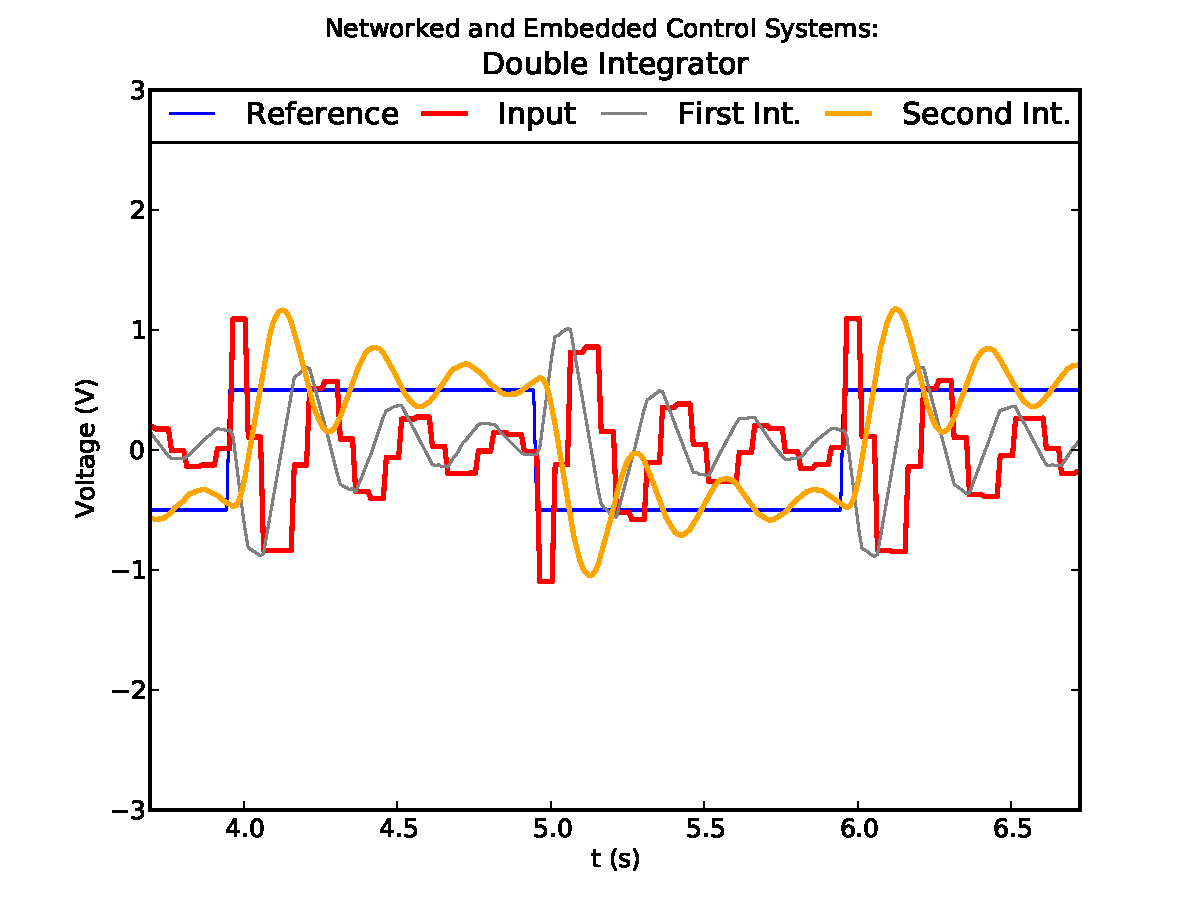
\includegraphics[width=0.85\linewidth]{necs_di_graph}
%	}
%	\\
%	\subfloat[Amb el bus CAN saturat de missatges, amb textos en català, només amb línies de referència i segona integral i en format PDF.]{\label{di_saturat_ref_segona_cat}
%		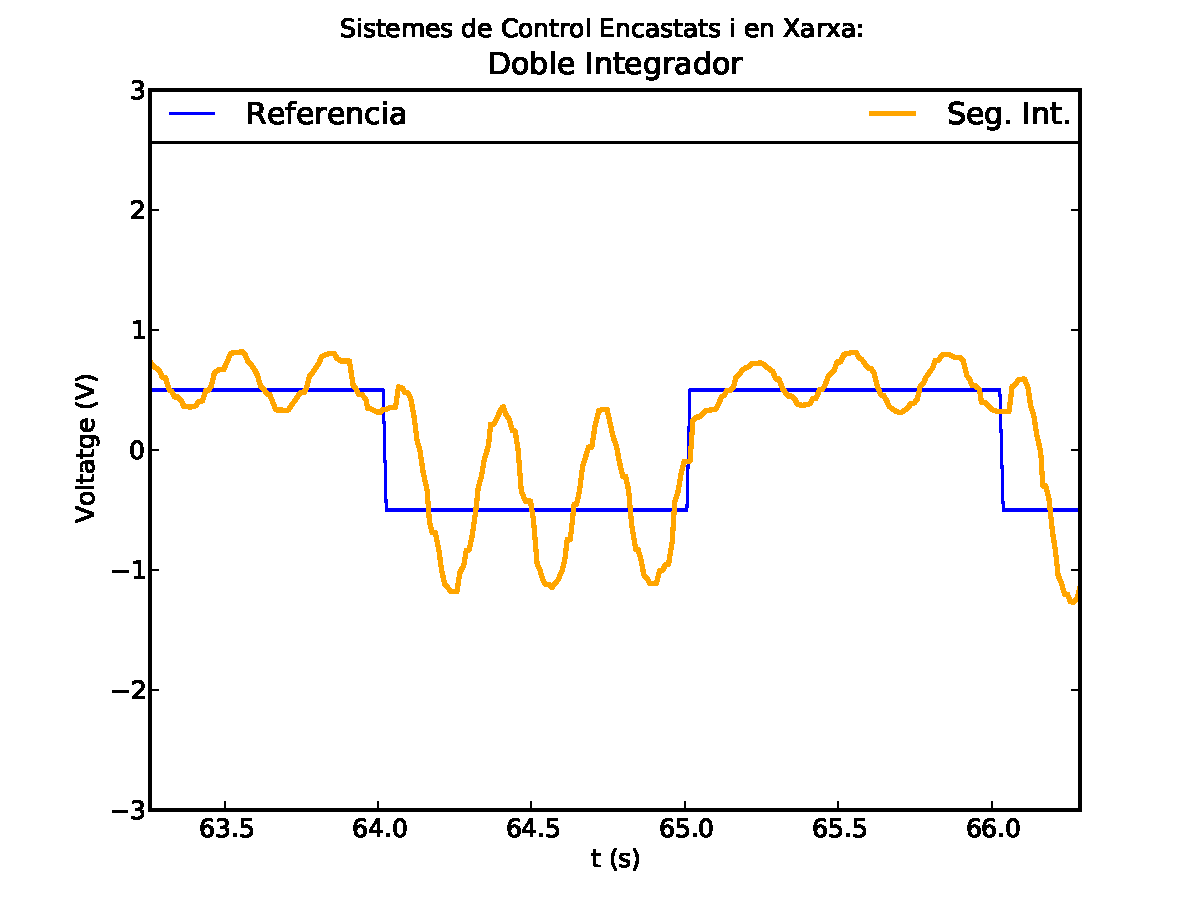
\includegraphics[width=0.85\linewidth]{di_saturat_ref_segona_cat}
%	}

%	\caption[Diferents gràfiques generades amb el programa \DCSMonitor]{Diferents gràfiques generades amb el programa \DCSMonitor del control d'un doble integrador.}
%    \label{fig:comparacio:graph}
%\end{figure}


%\begin{figure}[tbp]
%\centering
%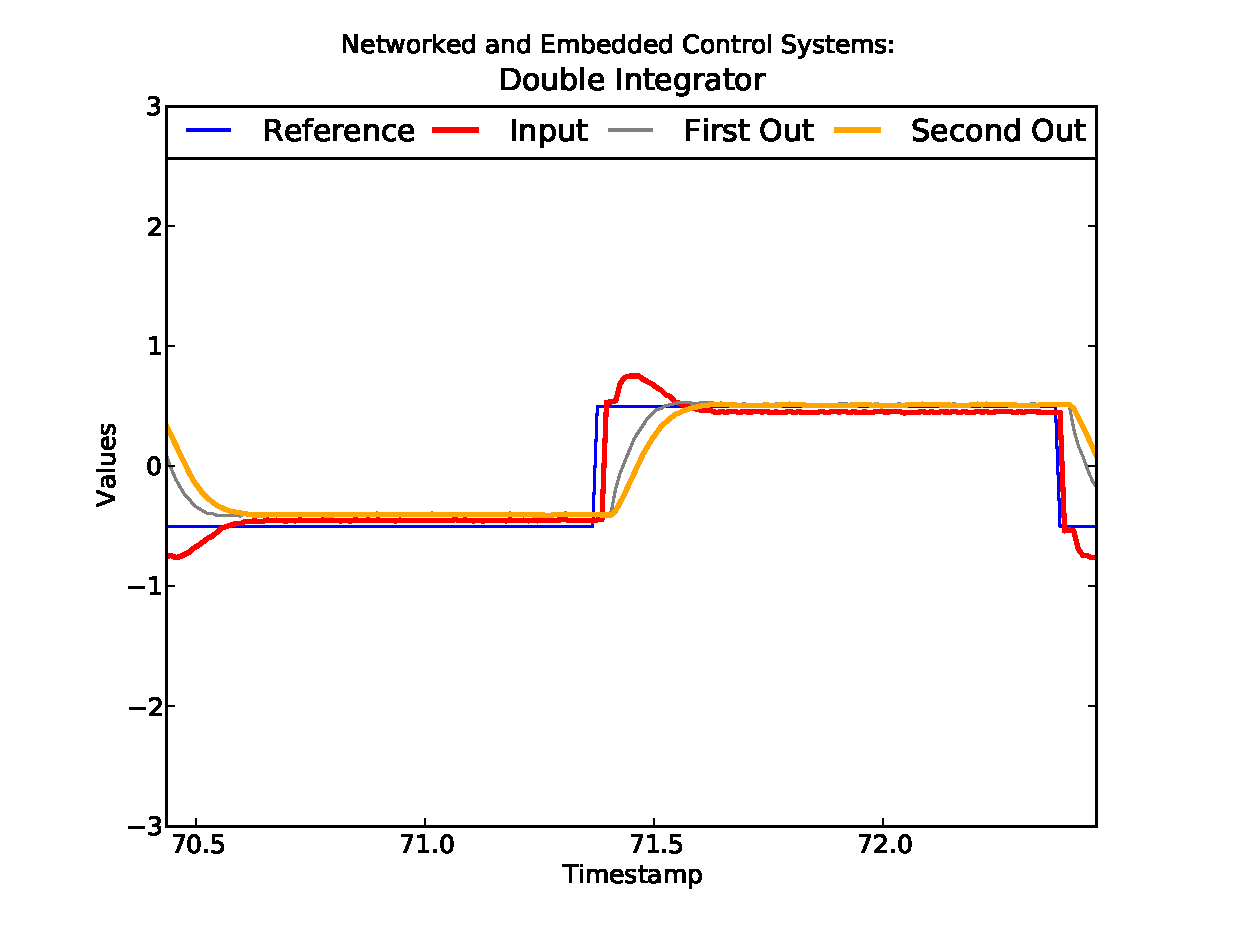
\epsfig{file=grup_12_eps.eps,width=0.9\linewidth,clip=}
%\caption{A title of some sort}
%\label{fig:aNicePicture}
%\end{figure}

%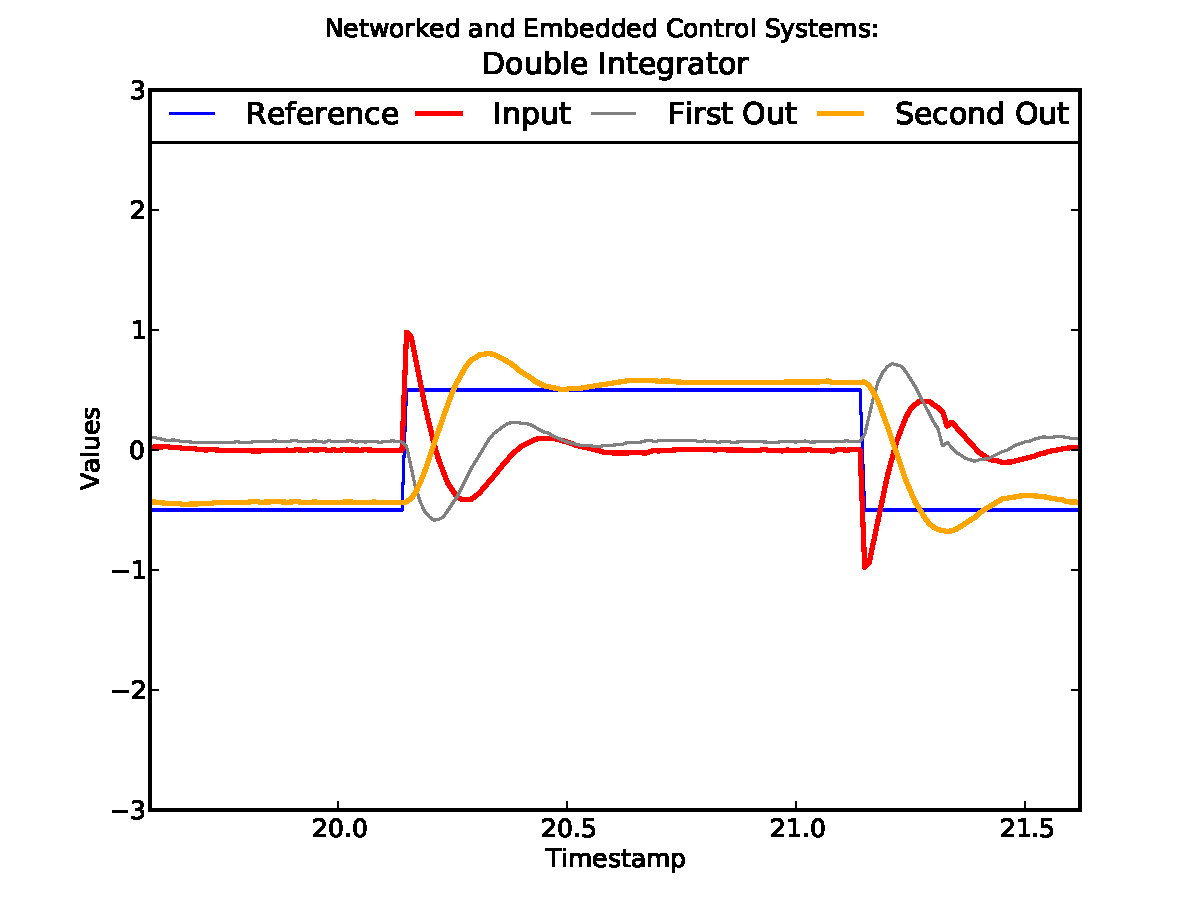
\includegraphics{3_laboratory_design/figures/grup_1_pdf.pdf}


%====================================================================================%
% Idiomes
%====================================================================================%
\subsection{Idiomes}\label{cap:dis:idi}

Un dels requisits que es buscava complir en el nou laboratori era que el programa visual fos multilingüe per tal de poder ser distribuït més fàcilment podent realitzar el laboratori en diferents parts del món.

Per tant es va estudiar la manera de realitzar aquest requisit de forma escalable i que fos ampliable fàcilment. Així que es va trobar una combinació de programes que podien realitzar aquesta tasca d'aquesta manera.

\begin{itemize}
	\item PyQT4 : Amb aquesta llibreria de \Python podem crear tot l'entorn visual del programa \DCSMonitor, i també ens permetrà fer la integració de les gràfiques (referent al idioma veure capítol \ref{cap:imp:idi:pyqt4}).
	\item Pylupdate4 : Amb aquest programa podrem generar fitxers entendibles per QtLingüist per tal de traduir tots els textos  que vulguem del programa (veure capítol \ref{cap:imp:idi:pylupdate4}).
	\item QtLingüist : Amb aquest programa es poden editar fàcilment els fitxers generats amb Pylupdate4, i un cop traduïts es genera un fitxer que la llibreria PyQT4 podrà interpretar en temps d'execució (veure capítol \ref{cap:imp:idi:qtlinguist})
\end{itemize}

Gràcies a totes aquestes eines el programa \DCSMonitor (que s'executa a l'ordinador) serà capaç de mostrar la informació essencial en varis idiomes, i és fàcilment ampliable ja que s'ha realitzat de forma estructurada per tal que seguint algunes instruccions es puguin generar més idiomes.

Actualment està traduït en els següents idiomes, però la llista pot ser fàcilment ampliada:

\begin{itemize}
	\item Català
	\item Espanyol
	\item Anglès
	\item Francès
\end{itemize}


%====================================================================================%
% Conclusions
%====================================================================================%
\section{Conclusions}\label{cap:dis:conc}

Al llarg d'aquest capítol hem pogut veure més profundament de que tracta el laboratori actual, i en quins punts es quedava curt. Tot seguit hem proposat un entorn en el que tots els llaços de control estiguessin en el mateix bus, i d'aquesta manera hem vist que necessitàvem dissenyar un ordre d'identificadors CAN que solucionessin els conflictes entre dispositius. Així que hem creat identificadors de missatges CAN amb alta prioritat per poder mantenir els controls més estables, i missatges en canvi menys prioritaris, que s'ocuparan exclusivament d'ocupar la resta del bus, sense perjudicar en cap moment el control.

També hem organitzat els diferents senyals de comunicació serie per RS232 per poder demanar l'execució de diferents accions al dispositiu \Monitor, i quin tipus d'accions volem que aquest sigui capaç de realitzar.

Amb tot això ven clar hem pogut dissenyar la interfície del programa \DCSMonitor, que ens ha de proporcionar informació de manera fàcil, i poder interactuar amb ell de manera intuïtiva.

Hem pogut veure mètodes per generar les gràfiques del control en temps real, i la seva exportació en diversos formats.

I per finalitzar hem vist que podem realitzar el programa \DCSMonitor multilingüe amb la utilització de varis programes, i seguint un cert ordre en la obtenció dels fitxers de traducció finals.

Ara que ja hem pogut veure la fase de disseny es l'hora d'implementar tots els sistemes, aquesta part es una de les més llargues, ja que moltes de les eines a utilitzar són noves i fer tasques senzilles poden comportar temps llargs. El que es veurà en la següent secció es el resultat de la implementació de tota la fase de disseny que hem vist. I algunes captures del programa final.
			
%%==================================================================%%
%% Author : Perelló Nieto, Miquel                                   %%
%% Version: 1.0, 04/11/2011                                         %%
%%                                                                  %%
%% Memoria del Projecte de Final de Carrera                         %%
%% Disseny del laboratori                                           %%
%%==================================================================%%

\chapter{Implementació del laboratori}\label{cap:imp}


% the code below specifies where the figures are stored
\ifpdf
    \graphicspath{{4_laboratory_implement/figures/PNG/}{4_laboratory_implement/figures/PDF/}{4_laboratory_implement/figures/}}
\else
    \graphicspath{{4_laboratory_implement/figures/EPS/}{4_laboratory_implement/figures/}}
\fi


% ----------------------- contents from here ------------------------

En aquest apartat aprofundirem en cóm s'ha dut a terme la programació de les diferents parts que conformen el laboratori que hem dissenyat anteriorment (capítol \ref{cap:dis}), i podrem veure d'aquesta manera com podem modificar el codi per ampliar el laboratori amb una infinitud de opcions, modificant o afegint diferents dispositius, o missatges de comunicació.

Per implementar el laboratori hem necessitat crear l'entorn necessari per compartir el bus CAN entre varis llaços de control, i tenir el programa \DCSMonitor connectat al dispositiu \Monitor via RS232, per tant existeix una configuració bàsica formada per dos llaços de control monitoritzats per un dispositiu \Monitor i aquest connectat al programa \DCSMonitor capaç de modificar el comportament d'aquest ultim. Es pot veure una fotografia de tot l'entorn preparat i configurat per tal de treballar amb aquest sistema, i amb el qual s'ha pogut dur a terme tota la fase de implementació (figura \ref{workspace}).

\figuremacro{workspace}{Entorn de treball}{Tot el material necessari per implementar el laboratori amb dos llaços de control, un programador Mplab ICD2, un conversor de RS232 a USB, el programa \DCSMonitor en marxa al monitor esquerra i codi font al monitor de la dreta.}

Hem dividit el capítol en dues seccions principals, la part de programació en \Python del programa \DCSMonitor (el programa que s'executa en l'ordinador) on podrem veure els passos que s'han seguit per crear la interfície visual (secció \ref{cap:imp:visual}), com hem pogut obrir el port RS232 i posteriorment enviar i rebre tot tipus de missatges (secció \ref{cap:imp:com:serie}), com hem integrat els plots del llaç de control que estiguéssim monitoritzant o  connectats (secció \ref{cap:imp:gen:graph}), com hem fet per exportar una gràfica generada en diferents formats (seccio \ref{cap:imp:exp:graph}), com hem realitzat l'actualització de les estadístiques en temps real (secció \ref{cap:imp:estat}), i finalment quins són els passos seguits per implementar els diferents idiomes, i per afegir-ne de nous (secció \ref{cap:imp:idi}). 

I la part de programació en \C en el Sistema Operatiu en Temps Real Erika Enterprise que corre en els diferents dispositius del control (microcontroladors dsPIC33FJ256MC710, en la placa \FLEX), on es podrà veure com implementar noves tasques en el SO Erika (secció \ref{lab:imp:dspic:monitor:tasks}), com hem implementat la recepció i enviament dels diferents missatges per RS232 (secció \ref{cap:imp:com:serie}), i el més important en els sistemes distribuïts la comunicació mitjançant el bus CAN (secció \ref{lab:imp:dspic:can}); la creació de màscares i filtres, la recepció dels diferents missatges, l'enviament d'aquests, i la creació de una pila per mantenir un llistat de tots els llaços de control presents al bus.

\FloatBarrier

\section{\DCSMonitor}\label{cap:imp:dcs}

Com hem vist anteriorment, el programa \DCSMonitor és l'encarregat de mostrar-nos en temps real el funcionament dels diferents controls als que estem connectats via RS232.
Gracies a ell podem monitoritzar un bus CAN (si estem connectats a un dispositiu \Monitor), o podem comprovar que el control que estem executant sigui correcte (connectats directament a un dispositiu \SensorActuador).
En aquest apartat s'explica com s'han programat totes les parts implicades del laboratori que formen part del programa \DCSMonitor, començant per l'aspecte visual, passant per les comunicacions i el mostreig dels plots, i acabant finalment per la integració amb varis idiomes.

Cal indicar que per crear les gràfiques en temps real s'ha pres com a exemple el codi de Yassine Benabbas amb Llicencia Creative Commons present en la bibliografia \cite[Creér un graphe dynamique avec PyPlot]{yassine}.

%====================================================================================%
% Interficie
%====================================================================================%
\subsection{Interficie}\label{cap:imp:visual}

Pel disseny de la part visual del programa es va utilitzar la eina \QTCreator, el qual és un IDE per realitzar interfìcies de programes arrossegant i enganxant les diferents parts. Això ens permet guanyar temps en petits programes, i en programes grans és quasi impossible prescindir d'aquesta ajuda.

Un cop hem realitzat la organització de tots els botons i etiquetes que formen el programa, li indiquem a \QTCreator que ens generi el codi font d'aquest en format \textit{.ui} (es posa un fragment de codi com a exemple, \ref{lab:imp:dsc:interficie:ui}, ja que el codi complert ocupa unes 700 línies, més o menys 25 pàgines)

\begin{code_xml}{Fragment del fitxer d'interficie dcsmmainwindow.ui}{lab:imp:dsc:interficie:ui}
<?xml version="1.0" encoding="UTF-8"?>
<ui version="4.0">
 <class>MainWindow</class>
 <widget class="QMainWindow" name="MainWindow">
  <property name="geometry">
   <rect>
    <x>0</x>
    <y>0</y>
    <width>752</width>
    <height>790</height>
   </rect>
  </property>
  <property name="windowTitle">
   <string>Distributed Control Systems Monitor</string>
  </property>
     ...
\end{code_xml}

Un cop hem generat aquest fitxer és hora de traduir-ho a \Python, per tal de que la llibrería que utilitzem \PyQT pugui generar l'interficie. Per fer aixó ens ajudem del programa \pyuic que amb la comanda \ref{lab:imp:pyuic4} genera un fitxer com el del fragment \ref{lab:imp:interficie:py}

\begin{code_bash}{Creant fitxer d'interficie}{lab:imp:pyuic4}
pyuic4 dcsmmainwindow.ui > dcsmmainwindow.py
\end{code_bash}

\begin{code_python}{Fragment de codi del fitxer dcsmmainwindow.py}{lab:imp:interficie:py}
try:
    _fromUtf8 = QtCore.QString.fromUtf8
except AttributeError:
    _fromUtf8 = lambda s: s

class Ui_MainWindow(object):
    def setupUi(self, MainWindow):
        MainWindow.setObjectName(_fromUtf8("MainWindow"))
        MainWindow.resize(752, 790)
        self.centralwidget = QtGui.QWidget(MainWindow)
\end{code_python}

Finalment es pot veure a la figura \ref{exemple_saturat_03} el resultat d'aquests passos, amb una captura de la pantalla de l'execució.
\begin{landscape}
\figuremacroW{exemple_saturat_03}{Interfície final del programa \DCSMonitor}{Captura de pantalla del programa \DCSMonitor mostrant el control amb el bus CAN saturat al 89\%, sense el plot de la primera integral i en anglès.}{1.4}
\end{landscape}

\FloatBarrier

%====================================================================================%
% Comunicació sèrie RS232
%====================================================================================%
\subsection{Comunicació sèrie RS232}\label{cap:imp:com:serie}

Ja hem vist en la secció de disseny dels tipus de missatge serie \ref{cap:dis:comSer} els diferents missatges que han de enviar-se entre el programa \DCSMonitor i els dispositius, ara veurem com hem implementat aquest tipus de comunicacions per la part de l'ordinador.

En aquest apartat indicarem com hem fet per configurar el port serie amb \PySerial, els mètodes que hem utilitzat per enviar els senyals al dispositiu connectat, i com hem rebut els valors necessaris per poder mostrar les gràfiques o llistar els diferents llaços del bus CAN.

%====================================================================================%
% Obrinr dispositiu
%====================================================================================%
\subsubsection{Obrir i tancar dispositiu sèrie}\label{cap:imp:com:serie:openclose}

Per utilitzar aquest tipus de comunicació primer de tot hem de decidir alguns dels paràmetres que porta associats el tipus de comunicació serie. Com anteriorment en el laboratori ja es van ajustar aquests paràmetres el que farem és adaptar-nos a ells i configurar el dispositiu tal i com estava funcionant.

Per fer això primer de tot importem el paquet serial de \Python, i tot seguit assignem els valors als diferents paràmetres (codi \ref{cap:imp:com:serie:conf:code}).

\begin{code_python}{Codi per configurar dispositiu sèrie}{cap:imp:com:serie:conf:code}
# for communicate with pic
import serial

PORT = '/dev/ttyUSB0'
BAUDRATE = 115200
BYTESIZE = serial.EIGHTBITS
PARITY = serial.PARITY_NONE
STOPBITS = serial.STOPBITS_ONE
TIMEOUT = 10
\end{code_python}

Amb tots els paràmetres ben instanciats, ja podem esperar el senyal de connexió per activar aquest dispositiu. El metode que s'utilitza és mitjançant un botó a la interfície del programa, la qual està enllaçada amb un senyal.
En el moment en el que el botó sigui premut, s'activarà la funció que li hem indicat (codi \ref{cap:imp:com:serie:openclose:trig:code}).

\begin{code_python}{Disparador de connexió de port serie}{cap:imp:com:serie:openclose:trig:code}
QtCore.QObject.connect(self.pushButton_connect, QtCore.SIGNAL("clicked()"), self.clicked_connect)
\end{code_python}

La funció amb la que està enllaçada el botó comprovarà si s'està activant o s'està desactivant. Si es prem per activar el dispositiu, provarà d'activar el port serie cridant a la funció \emph{connect\_serial} (codi \ref{cap:imp:com:serie:openclose:connect:code}, explicat més endavant), si això te èxit habilitarà tots els botons que estiguin permesos segons el mode d'execució en el que es trobi el programa (PC$->$\SensorActuador o PC$->$\Monitor) (figura \ref{serie_connectat}), en cas contrari marcarà en vermell que no s'ha pogut connectar (figura \ref{serie_error}).

En el cas en que s'estigui desconnectant el dispositiu serie, aturarà tots els events periòdics que estiguin activats (recepció de dades, dibuix de la gràfica i calcul d'estadístiques), tanca el dispositiu serie, i finalment desactivarà tots els botons que no calen usar.

\begin{code_python}{Codi per obrir/tancar dispositiu sèrie}{cap:imp:com:serie:openclose:buton:code}
def clicked_connect(self):
	if not self.pushButton_connect.isChecked():
		self.timer_graph.stop()
		self.timer_data.stop()
		self.timer_statistics.stop()
		self.ser.close()
		self.ser = 0
		self.lineEdit_state.setPalette(QtGui.QPalette(QtGui.QColor("gray")))
		self.lineEdit_state.setText(QtGui.QApplication.translate("MainWindow", "Disconnected", None, QtGui.QApplication.UnicodeUTF8))
		self.pushButton_connect.setText(QtGui.QApplication.translate("MainWindow", "Connect", None, QtGui.QApplication.UnicodeUTF8))
		self.pushButton_monitor.setEnabled(0)
		self.pushButton_monitor.setChecked(0)
		self.pushButton_reload.setEnabled(0)
		self.slider_saturation.setEnabled(0)
		
	else:
		if self.connect_serial():
		    self.lineEdit_state.setPalette(QtGui.QPalette(QtGui.QColor("green")))
		    self.lineEdit_state.setText(QtGui.QApplication.translate("MainWindow", "Connected", None, QtGui.QApplication.UnicodeUTF8))
		    self.pushButton_connect.setText(QtGui.QApplication.translate("MainWindow", "Disconnect", None, QtGui.QApplication.UnicodeUTF8))
		    self.pushButton_monitor.setEnabled(1)
		    self.slider_saturation.setEnabled(1)
		    if self.actionPC_Monitor.isChecked():
		        self.pushButton_reload.setEnabled(1)
		else:
		    self.lineEdit_state.setPalette(QtGui.QPalette(QtGui.QColor("red")))
		    self.lineEdit_state.setText(QtGui.QApplication.translate("MainWindow", "Error connecting", None, QtGui.QApplication.UnicodeUTF8))
		    self.pushButton_connect.setChecked(0)
\end{code_python}


La funció \emph{connect\_serial} és l'encarregada de connectar el dispositiu serie, primer de tot comprova si el dispositiu ja havia estat engegat algun cop. Si no ho havia estat li assigna tots els paràmetres anteriorment instanciats, i posteriorment intenta connectar. En cas de error la funció retornarà 0, en cas contrari retornarà 1.
En cas que el dispositiu ja hagués estat obert anteriorment, la configuració ja està instanciada, per tant només provarem d'obrir-la de nou. Igual que abans retornarà zero o u segons hagi fracassat o connectat amb èxit (codi \ref{cap:imp:com:serie:openclose:connect:code}).

\begin{code_python}{Codi per connectar port serie}{cap:imp:com:serie:openclose:connect:code}
def connect_serial(self):
        """Connects to the serial device, if not return 1"""
        if self.ser == 0:
            try:
                self.ser = serial.Serial(PORT, BAUDRATE, BYTESIZE, PARITY, STOPBITS, TIMEOUT)
                #self.ser = serial.Serial('/dev/ttyUSB0', 115200, timeout=10)
            except:
                self.textBrowser.append(QtGui.QApplication.translate("MainWindow", "\n\t----Failed to connect to the device----\n", None, QtGui.QApplication.UnicodeUTF8))
                return 0
        # this code shouldn't be never executed
        else:
            try:
                self.ser.open()
            except:
                self.textBrowser.append(QtGui.QApplication.translate("MainWindow", "\n\t----Failed to connect to the device----\n", None, QtGui.QApplication.UnicodeUTF8))
                return 0
        return 1
\end{code_python}

Tot seguit es pot veure els canvis que s'efectuen durant la connexió del port serie, en la primera imatge abans de connectar al dispositiu \emph{/dev/ttyUSB0}, després un cop ja s'ha establert la connexió, un cop hem desconnectat correctament el port, i la ultima imatge quan hi ha algun problema de connexió (figura \ref{fig:comparacio:rs232}).

\begin{figure}[ht!]
	\subfloat[Pendent de connectar.]{\label{serie_pendent}
		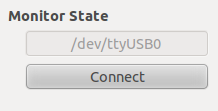
\includegraphics[width=0.25\linewidth]{serie_pendent}
	}
	\subfloat[Connectat correctament.]{\label{serie_connectat}
		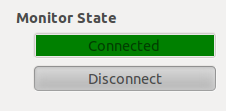
\includegraphics[width=0.25\linewidth]{serie_connectat}
	}
	\subfloat[Desconnectat correctament.]{\label{serie_desconnectat}
		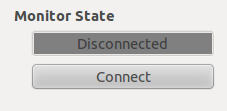
\includegraphics[width=0.25\linewidth]{serie_desconnectat}
	}
	\subfloat[Error al connectar.]{\label{serie_error}
		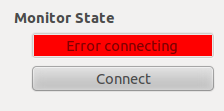
\includegraphics[width=0.25\linewidth]{serie_error}
	}
	\caption{Estat de connexió amb el \Supervisor via RS232.}
    \label{fig:comparacio:rs232}
\end{figure}

\FloatBarrier

%====================================================================================%
% Enviar petició de llistar dispositius
%====================================================================================%
\subsubsection{Enviar petició de llistar llaços de control}\label{cap:imp:com:serie:send:devices}

Al connectar el programa \DCSMonitor amb un dispositiu \Monitor el que ens interessa primer de tot és veure una llista dels diferents llaços de control existents al bus CAN. Aquesta acció només es pot iniciar quan el port serie esta degudament connectat i si el programa s'està executant en mode PC$->$Monitor, per aquest motiu el botó que permet fer aquesta crida romandrà si no es compleixen aquestes dues premisses.

Per activar-ho s'ha creat un disparador que enllaça el botó \emph{Llistar} amb la funció \emph{toogled\_reload} (codi del disparador \ref{cap:imp:com:serie:send:devices:trig:code}).

\begin{code_python}{Disparador de botó llistar dispositius}{cap:imp:com:serie:send:devices:trig:code}
QtCore.QObject.connect(self.pushButton_reload, QtCore.SIGNAL(_fromUtf8("clicked()")), self.toggled_reload)
\end{code_python}

Primer de tot al entrar a aquesta funció (codi \ref{cap:imp:com:serie:send:devices:code})comprova que estem correctament connectats al port serie, si no és així atura aquest procés. Si en canvi tot és correcte, comprova si estem aturant o estem iniciant la recepció d'identificadors, així que segons el que estem realitzant codificarà un o un altre missatge per després enviar-lo pel port serie (les codificacions és poden veure en la figura \ref{fig:bit_encoding:percent} del capítol de disseny)

En el cas de començar a demanar els identificadors, s'activa una alarma periòdica la qual està enllaçada a una funció que captura els missatges que es reben al port serie. Aquesta recepció es pot veure en la secció \ref{cap:imp:com:serie:rec:devices}.
En el cas de aturar aquesta petició, comprovarà si s'està monitoritzant, en cas negatiu aturarà la recepció de dades.

\begin{code_python}{Codi per demanar una llista de llaços de control}{cap:imp:com:serie:send:devices:code}
def toggled_reload(self):
    """Stops or Start to recive devices id's"""
    if not self.connect_serial():
        self.pushButton_reload.setChecked(0)
        return
        
    if self.pushButton_reload.isChecked():
        self.listWidget_link.clear()
        word = struct.pack("BBBBBBBB", ID_DEVICES,0,0,0,0,0,0,0)
        self.timer_data.start(DATA_TIME)
        
    else:
        word = struct.pack("BBBBBBBB", ID_DEVICES + ID_STOP,0,0,0,0,0,0,0)
        if (not self.pushButton_monitor.isChecked()):
            self.timer_data.stop()
        
    self.textBrowser.append(QtGui.QApplication.translate("MainWindow", "Sent : ", None, QtGui.QApplication.UnicodeUTF8)+binascii.hexlify(word)+"\n")
    
    self.ser.write(word)
\end{code_python}




%====================================================================================%
% Enviar petició de monitorització
%====================================================================================%
\subsubsection{Enviar petició de monitorització}\label{cap:imp:com:serie:send:monit}

Aquesta és la acció principal sobre la que es bassa el programa, en el moment que volem veure la gràfica en temps real d'un llaç de control hem d'enviar aquesta petició al \Monitor. Però també podem estar connectats a un dispositiu \SensorActuador, però en aquest cas ; com ja hem explicat en seccions anteriors (secció \ref{diss:nou}); aquesta petició es perdrà, però posarem en marxa tota la part de recepció de dades.

Primer de tot creem el disparador que detectarà que s'ha premut el botó per monitoritzar (codi \ref{cap:imp:com:serie:send:monit:trig:code}), aquest cridarà la funció \emph{toogled\_monitor} (codi \ref{cap:imp:com:serie:send:monit:code}).

\begin{code_python}{Disparador de botó per monitoritzar}{cap:imp:com:serie:send:monit:trig:code}
QtCore.QObject.connect(self.pushButton_monitor, QtCore.SIGNAL("clicked()"), self.toggled_monitor)
\end{code_python}

Aquesta serà la funció detectarà si el que volem és aturar o començar la monitorització, en cas d'iniciar-la comprovarà si hi ha un identificador de llaç de control de la llista seleccionat. Si hi és formarem el missatge amb aquest identificador, en cas contrari monitoritzarem el llaç de control numero u. Tot seguit enviarem aquest senyal per el port serie, netejarem el buffer d'entrada per no confondre algun senyal residual anterior amb un de nou. Netegem la gràfica i activem una funció (\emph{get\_periodical\_data}, veure codi \ref{cap:imp:com:serie:rec:monitor:perio:code}) que rep periòdicament informació per el port serie i la emmagatzema en arrays (els quals ens permetran dibuixar la gràfica), i activa una altre tasca periòdica que en cas de existir dades noves en els arrays tornarà a dibuixar la gràfica (secció de generació de gràfiques en temps real \ref{cap:imp:gen:graph}).
En el cas que estem parant la monitorització aturarem la tasca periòdica que dibuixava la gràfica, i si no s'estan rebent identificadors també aturarem la recepció de dades.

\begin{code_python}{Codi per demanar monitoritzar un llaç de control}{cap:imp:com:serie:send:monit:code}
def toggled_monitor(self):
	"""Starts or Stops reciving data"""
	if self.pushButton_monitor.isChecked():
		
		if not self.connect_serial():
		    self.pushButton_monitor.setChecked(0)
		    return
		
		self.textBrowser.insertPlainText(QtGui.QApplication.translate("MainWindow", "\n\t----NEW MONITORING----\n", None, QtGui.QApplication.UnicodeUTF8))
		
		id_link = self.listWidget_link.selectedItems()
		if len(id_link):
		    id_link = int(id_link[0].text())
		else:
		    id_link = 1
		
		self.textBrowser.insertPlainText(QtGui.QApplication.translate("MainWindow", "link to monitor : ", None, QtGui.QApplication.UnicodeUTF8)+str(id_link)+"\n")
		
		word = struct.pack("BBBBBBBB", ID_MONITOR,0,0,0,0,0,0,id_link&0xFF)

		self.textBrowser.append(QtGui.QApplication.translate("MainWindow", "Sent : ", None, QtGui.QApplication.UnicodeUTF8)+binascii.hexlify(word)+"\n")

		self.ser.write(word)
		 
		# clear data of the serial port
		self.ser.flushInput()
		# clear graph
		self.clean_graph()
		# start timer data reception
		self.get_periodical_data()
		# start timer graphic refresh
		self.update_graph()
		
		self.pushButton_save.setEnabled(False)
	else:
		# send Monitor
		word = struct.pack("BBBBBBBB", ID_MONITOR+ID_STOP,0,0,0,0,0,0,0)

		self.textBrowser.append(QtGui.QApplication.translate("MainWindow", "Sent : ", None, QtGui.QApplication.UnicodeUTF8)+binascii.hexlify(word)+"\n")

		self.ser.write(word)
		
		self.ser.flushInput()
		
		# reload number of waiting chars in serial rx buffer
		self.label_rx_buff_value.setText(str(self.ser.inWaiting()))
		
		self.textBrowser.insertPlainText(QtGui.QApplication.translate("MainWindow", "\n\t----END MONITORING----\n", None, QtGui.QApplication.UnicodeUTF8))
		
		self.pushButton_save.setEnabled(True)
		
		if (not self.pushButton_reload.isChecked()):
		    self.timer_data.stop()
		self.timer_graph.stop()
\end{code_python}


%====================================================================================%
% Enviar percentatge de saturació
%====================================================================================%
\subsubsection{Enviar percentatge de càrrega}\label{cap:imp:com:serie:send:sat}

Igual que en els casos anteriors per enviar aquest missatge al dispositiu \Monitor ho farem a través d'un disparador (codi \ref{cap:imp:com:serie:send:sat:trig:code}). Peró així com en els anteriors casos s'havia de prémer un botó per activar-ho, en aquest cas hi ha una barra que en canviar de posició és la que agafarà el seu valor (veure figura {fig:comparacio:barra}) i cridarà a la funció \emph{percent\_changed} (codi de la funció \ref{cap:imp:com:serie:send:sat:code}).
La barra que activa aquest enviament només està habilitada en el cas que el programa \DCSMonitor estigui en mode PC$->$Monitor.

\begin{code_python}{Disparador de barra de càrrega}{cap:imp:com:serie:send:sat:trig:code}
QtCore.QObject.connect(self.slider_saturation, QtCore.SIGNAL(_fromUtf8("valueChanged(int)")), self.percent_changed)
\end{code_python}

Aquesta funció comprova abans de res si estem degudament connectats al port serie, si no ho estem s'atura, en cas positiu prepara el missatge de la forma vista en la secció de disseny \ref{cap:dis:comSer:percent}, i li envia pel port serie.
Aquesta funció no ha d'esperar cap tipus de dades per tant no activa cap tasca periòdica.

\begin{code_python}{Codi per demanar que saturi el bus CAN }{cap:imp:com:serie:send:sat:code}
def percent_changed(self, num):
    """Change de label percent value and send this information to the Monitor Flex"""
    self.label_percent_value.setNum(num)
    
    if not self.connect_serial():
            return
    
    if num != 0:
        word = struct.pack("BBBBBBBB", ID_PERCENT,0,0,0,0,0,0,num)
    else:
        word = struct.pack("BBBBBBBB", ID_PERCENT+ID_STOP,0,0,0,0,0,0,0)
    
    self.textBrowser.append(QtGui.QApplication.translate("MainWindow", "Sent : ", None, QtGui.QApplication.UnicodeUTF8)+binascii.hexlify(word)+"\n")
    
    self.ser.write(word)
\end{code_python}


\begin{figure}[ht!]
	\subfloat[Nivell de càrrega al 0\%]{\label{saturation_00}
		
\includegraphics[width=\linewidth]{saturation_00}
	}
	
	\subfloat[Nivell de càrrega al 89\%]{\label{saturation_89}
		
\includegraphics[width=\linewidth]{saturation_89}
	}
	
	\subfloat[Nivell de càrrega al 94\%]{\label{saturation_94}
		
\includegraphics[width=\linewidth]{saturation_94}
	}

	\caption{Barra lliscant de càrrega en diferents posicions.}
    \label{fig:comparacio:barra}
\end{figure}

\FloatBarrier

%====================================================================================%
% Recepció de valors monitoritzats
%====================================================================================%
\subsubsection{Recepció de valors monitoritzats}\label{cap:imp:com:serie:rec:monitor}

Per poder realitzar la recepció de moltes dades pel port serie, es fa necessari deixar algun proces escoltant contínuament al port serie, però no podem permetre que el nostre programa es dediqui exclusivament a aquesta tasca, ja que tenim una interfície que hem d'atendre, gràfiques a dibuixar, i botons, que poden ser activats o desactivats. Per aquesta raó primer de tot creem un temporitzador, que permeti fer aquesta recepció de manera intermitent, deixant temps per atendre les altres tasques. Per fer això creem aquest temporitzador, i li assignem un disparador, que activarà la funció \emph{get\_periodical\_data} cada cop que passi el temps que li indiquem (codi \ref{cap:imp:com:serie:rec:monitor:trig:code}).

\begin{code_python}{Temporitzador i disparador per rebre dades del port serie}{cap:imp:com:serie:rec:monitor:trig:code}
timer_data = QtCore.QTimer()
    
# Periodical tasks
QtCore.QObject.connect(self.timer_data, QtCore.SIGNAL("timeout()"), self.get_periodical_data)
\end{code_python}

Peró aquesta declaració que hem creat no s'activa per si sola, sinó que hem d'engegar el temporitzador quan el necessitem, per tant cada cop que necessitem rebre informació de un llaç de control, o que volem una llista dels diferents llaços que hi ha al bus CAN al clicar el botó adequat (i després de realitzar codi que hem explicat en anteriors seccions) acabarà cridant a la funció \emph{get\_periodical\_data} (codi \ref{cap:imp:com:serie:rec:monitor:perio:code}).

Aquesta funció és l'encarregada de comprovar que la temporització funciona correctament, reactivant-la o parant-la en el moment oportú. El que fa primer de tot es comprovar que un dels botons que indiquen rebre informació estigui premut (aquests botons es queden premuts fins que no es torna a clicar per segon cop), en cas contrari ha d'aturar aquesta periodicitat i per tant ja no activa el temporitzador.
Un cop sap que realment es vol rebre informació, comprova que s'hagi dibuixat ja la informació que hi havia pendent, si ja s'ha dibuixat torna a rebre dades cridant a la funció \emph{recive\_data} (codi de la funció \ref{cap:imp:com:serie:rec:monitor:rx:code}). Això és així per crear una zona d'exclusió mútua (també anomenada Mutex), que evitarà que intentem dibuixar la gràfica de dades que estan a mig omplir.
I finalment reactiva el temporitzador per tornar a executar la mateixa funció.

\begin{code_python}{Codi per reactivar l'adquisició de dades}{cap:imp:com:serie:rec:monitor:perio:code}
def get_periodical_data(self):
    """Updates the data"""
    if not self.pushButton_monitor.isChecked() and not self.pushButton_reload.isChecked():
        return
    
    if self.updated_data == 0 :
        # recive new serial data
        self.recive_data()
        
    # activate the periodical reception of data
    self.timer_data.start(DATA_TIME)
\end{code_python}

Finalment la funció encarregada en rebre les dades pel port serie és la funció \emph{recive\_data} (codi \ref{cap:imp:com:serie:rec:monitor:rx:code}). Aquesta funció procura agafar tota la informació que hi hagi pendent al buffer d'entrada del port serie. Tenint en compte que el dispositiu \Monitor i el \SensorActuador envien aquesta informació cada 10 milisegons, i nosaltres fem lectures com a mínim cada 5 milisegons, tenim temps per fer la lectura i seguir executant altres codis. Primer de tot busca el byte de capçalera; aquest byte és un 0x01 que està al principi de tots els missatges que el dispositiu ens envia. Un cop ha trobat aquest byte sap que te les dades alineades, i pot prosseguir a llegir el numero de bytes que li correspongui (segons estigui en mode PC$->$\SensorActuador o PC$->$\Monitor llegirà 23 o 71 bytes respectivament). Ja amb el numero de bytes llegits, comprova si el botó de monitorització esta premut, per tal de agafar les dades per dibuixar la gràfica o passar a rebre la llista de dispositius (el codi que falta està en la secció \ref{cap:imp:com:serie:rec:devices}, codi \ref{cap:imp:com:serie:rec:devices:code}).

En la majoria de casos aquest botó si que està premut, i per tant agafa els bytes en l'ordre correcte per formar totes les variables necessàries, prepara el text per mostrar per pantalla i l'escriu en la part inferior del programa (figura \ref{fig:comparacio:valors}). Després afegeix als arrays el nou valor, i en treu un si ha arribat al màxim.
Després modifica els valors que apareixen en les estadístiques i habilita la zona d'exclusió.

\begin{code_python}{Codi per rebre els valors monitoritzats}{cap:imp:com:serie:rec:monitor:rx:code}
def recive_data(self):
    """Get messages from the serial port"""
    # read all available data
    while self.ser.inWaiting() > self.INPUT_DATA_SIZE+1:
        data = array.array('c')
        # search the header
        data.append(self.ser.read(1))
        while data[0] != chr(1):
            data[0] = self.ser.read(1)
            
        # wait for all available data
        while self.ser.inWaiting() < (self.INPUT_DATA_SIZE-1):
            time.sleep(0.03);
            
        # recives data
        data = self.ser.read(self.INPUT_DATA_SIZE-1)
        
        # prove if you want graphical data
        if self.pushButton_monitor.isChecked():
            # decodes the data
            t  = struct.unpack('I', data[3]+data[2]+data[1]+data[0])
            r  = struct.unpack('f', data[4]+data[5]+data[6]+data[7])
            x0 = struct.unpack('f', data[8]+data[9]+data[10]+data[11])
            x1 = struct.unpack('f', data[12]+data[13]+data[14]+data[15])
            u  = struct.unpack('f', data[16]+data[17]+data[18]+data[19])
            
            self.time = t[0]*25e-9
            
            # prepare the string output
            aux_str  = " t = "+str(self.time)+"\t"
            aux_str += " r = "+str(r[0])+"\t"
            aux_str += " u = "+str(u[0])+"\t"
            aux_str += " x1 = "+str(x1[0])+"\t"
            aux_str += " x0 = "+str(x0[0])+"\n"
            # print string output
            self.textBrowser.insertPlainText(aux_str)
            
            # append data to the arrays
            self.graf_t.append(self.time)
            self.graf_r.append(r[0])
            self.graf_x0.append(x0[0])
            self.graf_x1.append(x1[0])
            self.graf_u.append(u[0])
            
            # remove one value if the arrays have maximum length
            if self.graf_t.buffer_info()[1] >= NUM_SAMPLES:
                self.graf_t.pop(0)
                self.graf_r.pop(0)
                self.graf_x0.pop(0)
                self.graf_x1.pop(0)
                self.graf_u.pop(0)
                  
            # reload number of samples lavel
            self.label_samples_value.setText(str(self.graf_t.buffer_info()[1]))
            # reload number of waiting chars in serial rx buffer
            self.label_rx_buff_value.setText(str(self.ser.inWaiting()))

            # reload mutex area
            self.updated_data = 1
\end{code_python}

\begin{figure}[ht!]
	\subfloat[Rebent els valors d'una monitorització.]{\label{valors_rebent}
		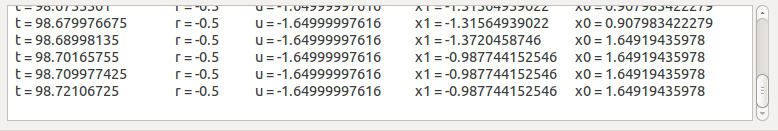
\includegraphics[width=\linewidth]{valors_rebent}
	}
	
	\subfloat[Havent finalitzat una monitorització.]{\label{valors_final}
		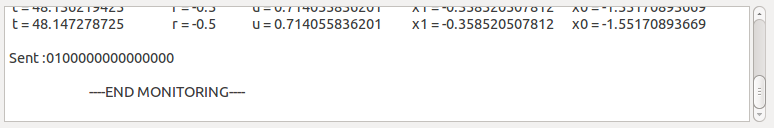
\includegraphics[width=\linewidth]{valors_final}
	}

	\caption{Espai de text per valors monitoritzats.}
    \label{fig:comparacio:valors}
\end{figure}

\FloatBarrier

%====================================================================================%
% Recepció de llista de dispositius
%====================================================================================%
\subsubsection{Recepció de llista de dispositius}\label{cap:imp:com:serie:rec:devices}

Per la recepció dels identificadors dels llaços de control com hem vist en l'apartat anterior \ref{cap:imp:com:serie:send:devices} s'activa la mateixa funció periòdica per rebre informació, per tant el codi que segueix és la continuació de la funció vista anteriorment \emph{recive\_data} (codi \ref{cap:imp:com:serie:rec:monitor:rx:code}).
Per tant seguint l'execució d'aquesta funció abans mencionada, comprovem si el byte 20 de les dades que ens arriben està a valor dos. En aquest cas significa que en el següent byte ve el nombre de identificadors diferents de mida un byte que el segueixen. Així que comprova un a un si ja es trobaven a la llista, i si no és així els afegeix.

\begin{code_python}{Codi per rebre la llista de dispositius }{cap:imp:com:serie:rec:devices:code}
....
# prove if there are available id's
if (self.actionPC_Monitor.isChecked() and data[20] == chr(2)):
    # if it is true, looks how much id's
    i  = struct.unpack('B', data[21])

    if i[0] < STACK_SIZE:
        for z in range(i[0]):
            new_device = struct.unpack('B', data[z+22])
            new_string = str(new_device[0])
            
            llista = self.listWidget_link.findItems(new_string, QtCore.Qt.MatchExactly)
            if len(llista) == 0:
                self.listWidget_link.addItem(new_string)
\end{code_python}

Es poden veure com a exemple algunes captures de pantalla de la llista abans de començar a demanar-li els identificadors (figura \ref{llista_cap}), actualitzant la llista en un bus amb dos llaços de control (figura \ref{llista_algun}), i la ultima imatge havent demanat la llista en un bus on existien varis llaços de control (figura \ref{llista_molts}).

\begin{figure}[ht!]
	\subfloat[Abans de demanar la llista.]{\label{llista_cap}
		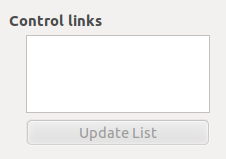
\includegraphics[width=0.3\linewidth]{llista_cap}
	}
	\subfloat[Amb dos llaços al bus CAN.]{\label{llista_algun}
		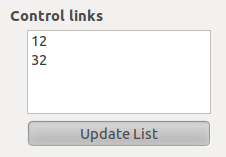
\includegraphics[width=0.3\linewidth]{llista_algun}
	}
	\subfloat[Amb molts llaços al bus CAN]{\label{llista_molts}
		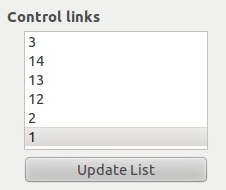
\includegraphics[width=0.3\linewidth]{llista_molts}
	}

	\caption{Llista de llaços de control al bus CAN.}
    \label{fig:comparacio:llista}
\end{figure}

\FloatBarrier

%====================================================================================%
% Generació de gràfiques en temps real
%====================================================================================%
\subsection{Generació de gràfiques en temps real}\label{cap:imp:gen:graph}

Generar aquestes gràfiques és un dels propòsits més importants del programa, i per tant ha de ser prou ràpida per no saturar el programa però al mateix temps donar una sensació visual de moviment.
Aquesta generació està associada a un temporitzador especific, enllaçat a un disparador que activa la funció \emph{update\_graph} (codi \ref{cap:imp:gen:graph:code}).
Aquest temporitzador s'activa només quan es prem el botó de monitorització, vist en la secció \ref{cap:imp:com:serie:send:monit}.

\begin{code_python}{Temporitzador i disparador per dibuixar la gràfica}{cap:imp:gen:graph:trig:code}
timer_graph = QtCore.QTimer()

# Periodical tasks
QtCore.QObject.connect(self.timer_graph, QtCore.SIGNAL("timeout()"), self.update_graph)
\end{code_python}

Un cop s'ha activat el temporitzador que crida aquesta funció, primer de tot comprova que hi hagi dades noves per dibuixar i que no s'estiguin modificant en aquest precís instant (això s'ha vist en la secció de recepció de dades \ref{cap:imp:com:serie:rec:monitor}). Si les dades que hi ha han estat actualitzades dibuixa primer les línies verticals i horitzontals que hi ha darrera dels plots. I després comprova un a un si hi ha marcada la opció de dibuixar els diferents plots (referència, primera i/o segona integral i valor d'entrada; figura \ref{fig:comparacio:plots}); segons quins estiguin activats, els crea i dibuixa o no. Finalment prova de pintar tot el que ha generat, actualitza la variable \emph{frames per second} per indicar que s'ha fet un nou dibuix i es marca la variable per la zona d'exclusió mútua perquè es puguin seguir afegint dades als arrays.
Finalment comprova que encara es vulgui seguir dibuixant la gràfica i es reactiva la temporització.
        
\begin{code_python}{Codi per actualitzar la gràfica }{cap:imp:gen:graph:code}
def update_graph(self):
    """Updates the graph"""
    # looks for new data
    if self.updated_data == 1:
                  
        self.mplWidget.canvas.ax.set_xbound(self.time-XLIM, self.time)
        self.mplWidget.canvas.draw()

        try:
            #Draw the lines
            if self.checkBox_R.isChecked():
                self.referenceLine.set_data(self.graf_t, self.graf_r)
                self.mplWidget.canvas.ax.draw_artist(self.referenceLine)
            if self.checkBox_x0.isChecked():
                self.x0Line.set_data(self.graf_t, self.graf_x0)
                self.mplWidget.canvas.ax.draw_artist(self.x0Line)
            if self.checkBox_U.isChecked():
                self.uLine.set_data(self.graf_t, self.graf_u)
                self.mplWidget.canvas.ax.draw_artist(self.uLine)
            if self.checkBox_x1.isChecked():
                self.x1Line.set_data(self.graf_t, self.graf_x1)
                self.mplWidget.canvas.ax.draw_artist(self.x1Line)
        except AssertionError:
            pass
            
        try:
            self.mplWidget.canvas.blit(self.mplWidget.canvas.ax.bbox)
        except AttributeError:
            pass
        
        self.fps = self.fps+1
        
        self.updated_data = 0
        
    if self.pushButton_monitor.isChecked() == 1:
        # activate the periodical update graph
        self.timer_graph.start(GRAPH_REFRESH)
\end{code_python}


\begin{figure}[ht!]
\begin{center}
	\subfloat[Abans alguns plots seleccionats.]{\label{alguns_seleccionats}
		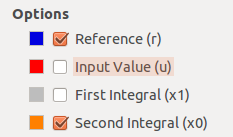
\includegraphics[width=0.35\linewidth]{alguns_seleccionats}
	}
	\subfloat[Amb tots els plots seleccionats.]{\label{tots_seleccionats}
		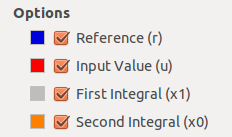
\includegraphics[width=0.35\linewidth]{tots_seleccionats}
	}
\end{center}
	\caption{Opció de plots per la gràfica.}
    \label{fig:comparacio:plots}
\end{figure}

\FloatBarrier

%====================================================================================%
% Exportar gràfica
%====================================================================================%
\subsection{Exportar gràfica}\label{cap:imp:exp:graph}

Exportar les gràfiques que s'estiguin monitoritzant en temps real és molt important, ja que gracies a això es pot guardar una captura de cada grup del laboratori, o generar imatges vectorials fàcilment introduïbles en articles o llibres (formats com .eps, .svg, .ps o .pdf).
Per poder generar aquestes imatges s'espera que es premi un botó, que està enllaçat mitjançant un disparador (codi \ref{cap:imp:exp:graph:trig:code}) a la funció que genera la imatge \emph{save\_image} (codi \ref{lab:imp:exp:graph:code}).

\begin{code_python}{Disparador per exportar la gràfica}{cap:imp:exp:graph:trig:code}
QtCore.QObject.connect(self.pushButton_save, QtCore.SIGNAL(_fromUtf8("clicked()")), self.save_image)
\end{code_python}

Un cop han activat aquesta funció primerament s'obra una finestra nova on es pot introduir el nom del nou fitxer a crear (figura \ref{exportant_nom}). A part de poder introduir el nom, podem llistar tots els fitxers dels diferents tipus que el programa és capaç de exportar, que hi hagin en el directori que estem observant. Per aquest motiu en la creació de la finestra apareixen descripcions d'aquests tipus de fitxers (figura \ref{exportant_tipus}).

\figuremacroW{exportant_nom}{Finestra per posar nom a la gràfica exportada}{}{0.9}

\figuremacroW{exportant_tipus}{Tipus de fitxer als que es pot exportar}{}{0.5}

Un cop l'usuari ha introduït el nom i clicat a acceptar començarem a generar una gràfica nova des de zero. Comprovarem un a un tots els plots que hem de dibuixar, afegint a la gràfica els que calguin.
Tot seguit indicarem quin rang de valors volem dibuixar, i posarem títol, subtítol, i noms als diferents eixos (tots aquests textos són traduïts a l'idioma que hi hagi seleccionat en el programa).
Després assigna algunes de les mides del dibuix, i finalment intenta guardar la imatge amb el nom i format que li hagim indicat anteriorment. Si per alguna raó fallés en aquesta tasca, procuraria guardar-lo en format \emph{.svg}.
Al acabar de generar la imatge aquesta gràfica nova es neteja per alliberar la memòria.

Un cop finalitzat el programa, el resultat de la captura de imatges és el que es pot observar en la figura \ref{fig:comparacio:graph}, en la que apareix una gràfica generada en anglès, amb totes les línies, i una altre en català només amb les línies de referència i de sortida del doble integrador.

\begin{figure}[ht!]
	\subfloat[Amb textos en anglès, totes els plots i en format PDF.]{\label{necs_di_graph}
		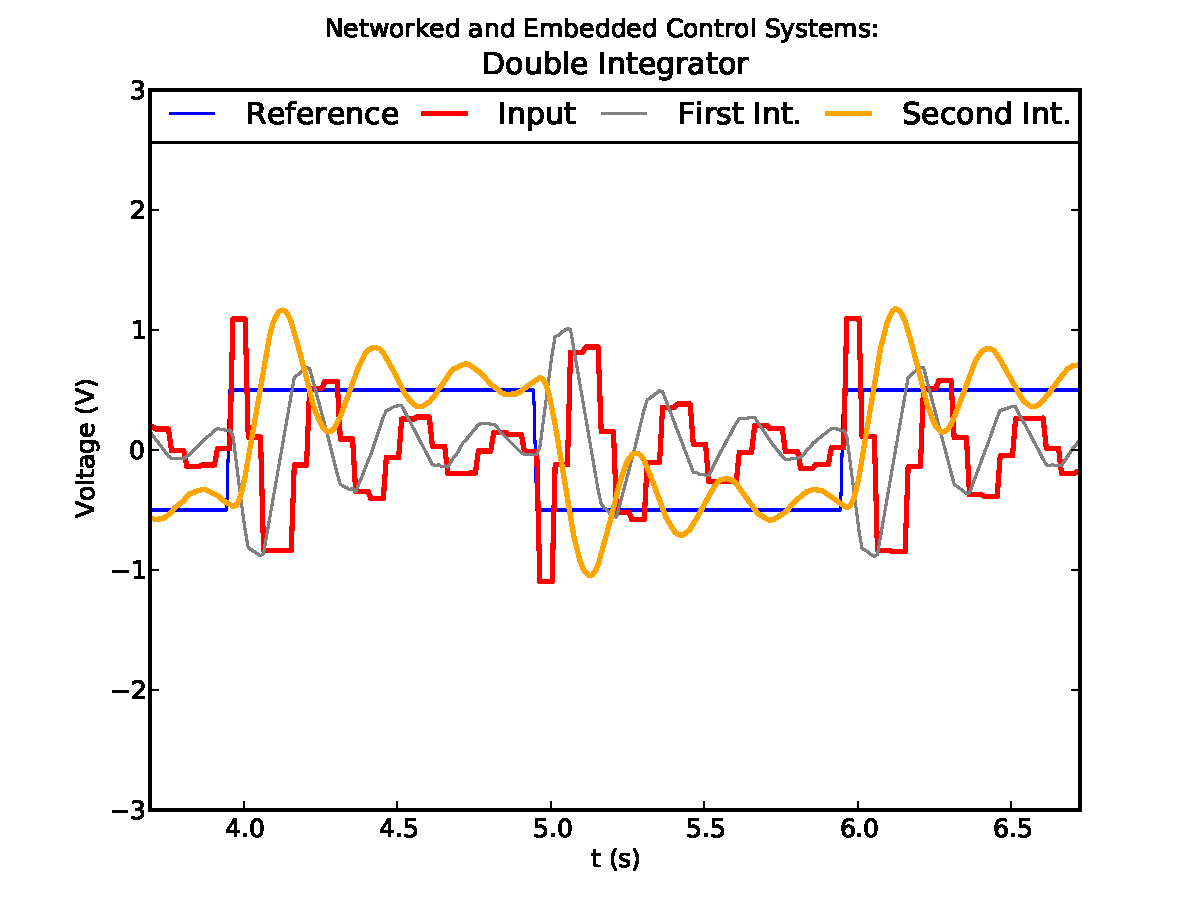
\includegraphics[width=0.88\linewidth]{necs_di_graph}
	}
	\\
	\subfloat[Amb el bus CAN carregat de missatges, amb textos en català, només amb plots de referència i segona integral i en format PDF.]{\label{di_saturat_ref_segona_cat}
		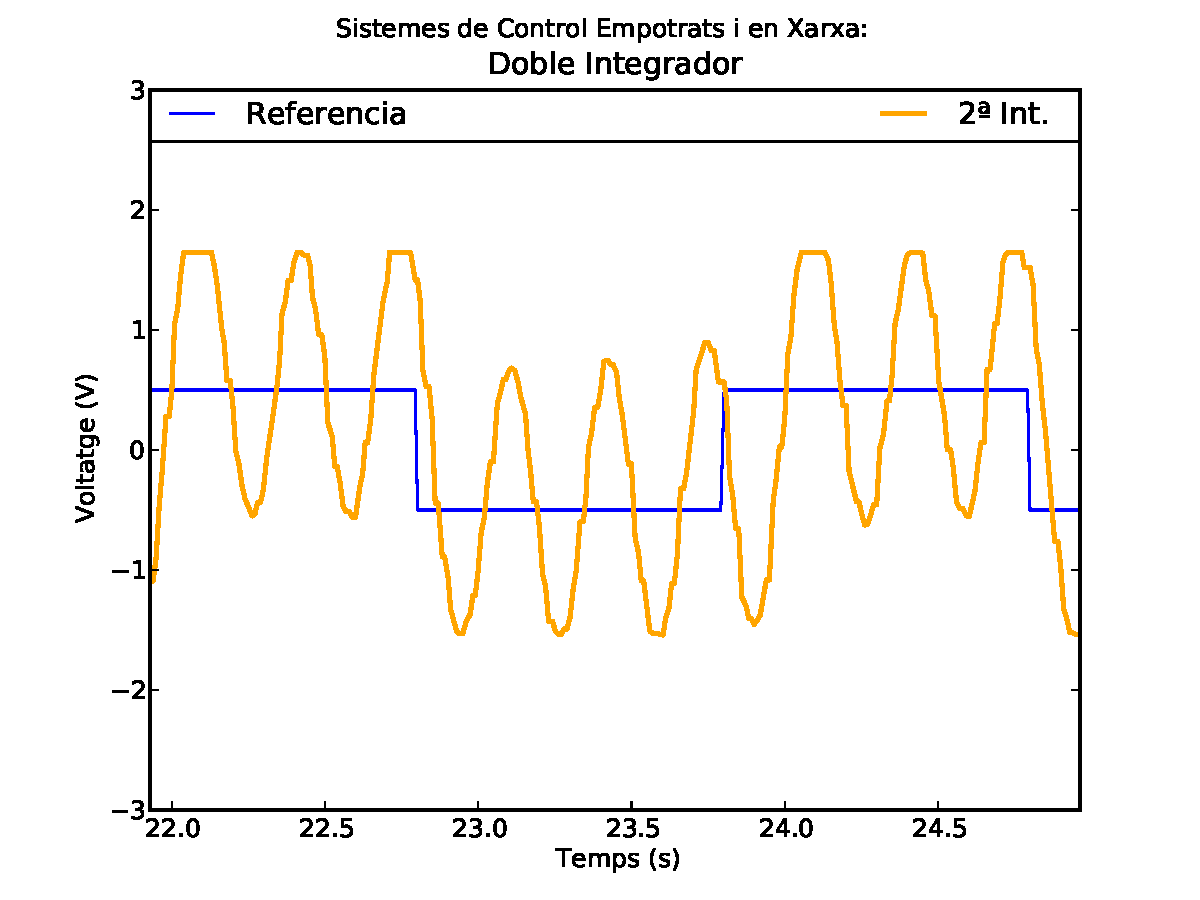
\includegraphics[width=0.88\linewidth]{di_saturat_ref_segona_cat}
	}

	\caption[Diferents gràfiques generades amb el programa \DCSMonitor]{Diferents gràfiques generades amb el programa \DCSMonitor del control d'un doble integrador.}
    \label{fig:comparacio:graph}
\end{figure}

\begin{code_python}{Codi per generar imatge d'una gràfica}{lab:imp:exp:graph:code}
def save_image(self):
    """Exports the graph into an image"""
    # open the dialog and get the selected file
    file_one = QtGui.QFileDialog.getSaveFileName(
         self,
         QtGui.QApplication.translate(
            "MainWindow", 
            "Supported formats:", 
            None, 
            QtGui.QApplication.UnicodeUTF8)+
            " emf, eps, pdf, png, ps, raw, rgba, svg, svgz", 
         "",
         "Enhanced MetaFile \t.emf (*.emf);; "+
         "Encapsulated PostScript \t.eps (*.eps);; "+
         "Portable Document Format \t.pdf (*.pdf);; "+
         "Portable Network Graphics \t.png (*.png);;"+
         "PostScript \t.ps (*.ps);; "+
         "RAW image file \t.raw (*.raw);; "+
         "Red Green Blue Alpha \t.rgba (*.rgba);; "+
         "Scalable Vector Graphics \t.svg (*.svg);; "+
         "Scalable Vector Graphics compressed \t.svgz (*.svgz)")
    # if a file is selected
    if file_one:
        # update the lineEdit text with the selected filename
        self.textBrowser.append(
            QtGui.QApplication.translate(
                "MainWindow", 
                "Saving to ", 
                None, 
                QtGui.QApplication.UnicodeUTF8
                )+file_one)

        plt.clf()
        # adding different plots if required
        if self.checkBox_R.isChecked():
            lines = plt.plot(self.graf_t, self.graf_r)
            plt.setp(lines[0], 
                     lw=1, 
                     label=str(
                        QtGui.QApplication.translate(
                            "MainWindow", 
                            "Reference",  
                            None, 
                            QtGui.QApplication.UnicodeUTF8)), 
                    color = 'blue')
            
        if self.checkBox_U.isChecked():
            lines = plt.plot(self.graf_t, self.graf_u)
            plt.setp(lines[0], 
                     lw=2, 
                     label=str(
                        QtGui.QApplication.translate(
                            "MainWindow", 
                            "Input",      
                            None, 
                            QtGui.QApplication.UnicodeUTF8)), 
                     color='red')
            
        if self.checkBox_x1.isChecked():
            lines = plt.plot(self.graf_t, self.graf_x1)
            plt.setp(lines[0], 
                     lw=1, 
                     label=str(
                        QtGui.QApplication.translate(
                            "MainWindow", 
                            "First Int.",  
                            None, 
                            QtGui.QApplication.UnicodeUTF8)), 
                     color='grey')
            
        if self.checkBox_x0.isChecked():
            lines = plt.plot(self.graf_t, self.graf_x0)
            plt.setp(lines[0], 
                     lw=2, 
                     label=str(
                        QtGui.QApplication.translate(
                            "MainWindow", 
                            "Second Int.", 
                            None, 
                            QtGui.QApplication.UnicodeUTF8)), 
                     color='orange')

        plt.axis([self.graf_t[0], self.graf_t[-1], -3, 3])
        
        plt.title(str(
            QtGui.QApplication.translate(
                "MainWindow", 
                "Double Integrator", 
                None, 
                QtGui.QApplication.UnicodeUTF8)))
        
        plt.suptitle(str(
            QtGui.QApplication.translate(
                "MainWindow", 
                "Networked and Embedded Control Systems:", 
                None, 
                QtGui.QApplication.UnicodeUTF8)))
        
        plt.xlabel(str(
            QtGui.QApplication.translate(
                "MainWindow", 
                "t (s)", 
                None, 
                QtGui.QApplication.UnicodeUTF8)))
        
        plt.ylabel(str(
            QtGui.QApplication.translate(
                "MainWindow", 
                "Voltage (V)", 
                None, 
                QtGui.QApplication.UnicodeUTF8)))
        
        plt.legend(bbox_to_anchor=(0, 1, 1, 0), loc=1, ncol=6, mode="expand", borderaxespad=0.)
               
        filename = str(file_one)# + '.svg'
        try:
            plt.savefig(filename, dpi=300)
        except ValueError as e:
            print(e)
            self.textBrowser.append(str(e))
            self.textBrowser.append(
                QtGui.QApplication.translate(
                    "MainWindow", 
                    "Trying to save as .svg", 
                    None, 
                    QtGui.QApplication.UnicodeUTF8))
            
            filename = str(file_one) + '.svg'
            plt.savefig(filename, dpi=300)
            pass
        except ImportError as e:
            print(e)
            self.textBrowser.append(str(e))
            self.textBrowser.append(
                QtGui.QApplication.translate(
                    "MainWindow", 
                    "Trying to save as .svg", 
                    None, 
                    QtGui.QApplication.UnicodeUTF8))
            
            filename = str(file_one) + '.svg'
            plt.savefig(filename, dpi=300)
            pass
        except:
            self.textBrowser.append("Error al guardar la imatge")
        
        plt.clf()
\end{code_python}

\FloatBarrier

%====================================================================================%
% Mostrant estadístiques
%====================================================================================%
\subsection{Mostrant estadístiques}\label{cap:imp:estat}

Com en la part de disseny es va explicar, periòdicament anirem creant estadístiques per saber que tot funciona correctament. 
Els valors que ens interessa saber en cada instant són: 

\begin{itemize}
	\item Nombre de llaços de control que hi ha connectats al bus CAN.
	\item Imatges per segon que es mostren en la gràfica en temps real.
	\item Nombre de mostres per plot dibuixat.
	\item Nombre de bytes esperant al buffer d'entrada del port serie.
	\item Marca canviant per saber que les estadístiques s'estan actualitzant periòdicament.
\end{itemize}

Per fer que aquestes estadístiques s'actualitzin periòdicament, com hem vist en altres seccions primer de tot hem de crear un temporitzador, i tot seguit li assignarem un disparador que activará la funció \emph{update\_statistics} (codi del disparador, i activació de les estadístiques \ref{cap:imp:est:trig:code}).

\begin{code_python}{Temporitzador i disparador per actualitzar les estadístiques.}{cap:imp:est:trig:code}
timer_statistics = QtCore.QTimer()

# Periodical tasks
QtCore.QObject.connect(self.timer_statistics, QtCore.SIGNAL("timeout()"), self.update_statistics)

self.timer_statistics.start(STAT_REFRESH)
\end{code_python}

El que fa la funció \emph{update\_statistics} (codi \ref{lab:imp:estat:update:code}) és primer de tot comprovar que el port serie estigui degudament connectat, si no és així no modifica cap valor estadístic, en cas contrari comença a actualitzant el nombre de mostres de tots els plots, el nombre de bytes pendents al port serie, el nombre d'imatges per segon que estan apareixent a la gràfica (si aquesta està aturada, força un dibuix cada cop, per si hi ha algun problema), actualitza el valor canviant per indicar que aquesta funció està funcionant correctament, actualitza el nombre de llaços de control que hi ha al bus CAN i finalment torna a reactivar la funció al cap de mig segon.

\begin{code_python}{Codi per generar i actualitzar les estadístiques.}{lab:imp:estat:update:code}
def update_statistics(self):
    """Update value of labels in statistics"""
    if self.ser != 0:
        # reload number of samples lavel
        self.label_samples_value.setText(str(self.graf_t.buffer_info()[1]))
        # reload number of waiting chars in serial rx buffer
        self.label_rx_buff_value.setText(str(self.ser.inWaiting()))
        
        self.label_fps_value.setText(str(self.fps*2))
        
        self.fps = 0
        
        if self.pushButton_monitor.isChecked() == 0:
            self.force_update_graph()
            
        if self.label_Est_value.text() != '(>_<)':
            self.label_Est_value.setText('(>_<)')
        else:
            self.label_Est_value.setText('(o_o)')
        
        self.label_T_value.setText(str(self.listWidget_link.count()))
        
        self.timer_statistics.start(STAT_REFRESH)
\end{code_python}

Tot seguit es poden veure diferents captures del canvi que es produeix en les estadístiques, primer es veu quan encara no està connectat al port serie, després al connectar però no tractar les dades que ens envia el dispositiu, després un cop estem tractant les dades rebudes i dibuixant la gráfica en temps real, i per ultim un cop hem aturat la monitorització del llaç de control (figura \ref{fig:comparacio_estadistiques}).

\begin{figure}[ht!]
	\subfloat[Pendent de començar.]{\label{estadistiques_pendents}
		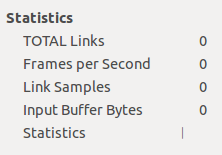
\includegraphics[width=0.24\linewidth]{estadistiques_pendents}
	}
	\subfloat[Connectat al dispositiu.]{\label{estadistiques_connect}
		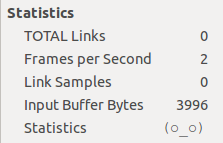
\includegraphics[width=0.24\linewidth]{estadistiques_connect}
	}
	\subfloat[Monitoritzant.]{\label{estadistiques_monitoritzant}
		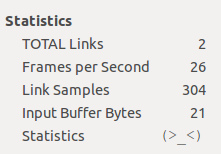
\includegraphics[width=0.24\linewidth]{estadistiques_monitoritzant}
	}
	\subfloat[Monitorització aturada.]{\label{estadistiques_desconnect}
		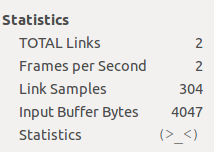
\includegraphics[width=0.24\linewidth]{estadistiques_desconnect}
	}
	\caption{Comparació dels valors estadístics.}
    \label{fig:comparacio_estadistiques}
\end{figure}

\FloatBarrier

%====================================================================================%
% Idiomes
%====================================================================================%
\subsection{Idiomes}\label{cap:imp:idi}

Un dels requisits que es buscava complir en el nou laboratori era que el programa visual fos multilingüe per tal de poder ser distribuït més fàcilment podent realitzar el laboratori en diferents països.

Així que el programa \DCSMonitor (que s'executa a l'ordinador) és capaç de mostrar tota la informació en varis idiomes, i és fàcilment ampliable ja que s'ha realitzat de forma estructurada per tal que seguint algunes instruccions es puguin generar més idiomes.

Com vam dir a l'apartat de disseny \ref{cap:dis:idi}, això ho hem aconseguit utilitzant una combinació de diferents eines amb les quals una rere l'altre ens generen el resultat desitjat. Tot seguit s'expliquen les diferents eines utilitzades, i com s'implementa cadascuna.

%====================================================================================%
% PyQT4
%====================================================================================%
\subsubsection{PyQT4}\label{cap:imp:idi:pyqt4}

Aquesta llibreria és l'encarregada de deixar-ho tot preparat perquè els textos del programa siguin traduits. Així que primerament, dintre de tot el codi del programa, es pot observar que tots els textos traduibles están envoltats amb la mateixa funció \emph{QtGui.QApplication.translate} (veure exemple en el codi \ref{lab:imp:idi:pyqt4:trans:example}).
Aquesta funció prepara tot l'entorn necessari per agafar tots aquests textos, i posteriorment mitjançant uns fitxers de traducció traduir en temps d'execució.
En aquest exemple li indiquem que la paraula "Sent : " volem que pugui ser traduïda, per tant cada cop que cridem aquesta funció amb aquesta estructura ens retornarà la paraula en l'idioma que tinguem carregat.

\begin{code_python}{Exemple de text per traduir}{lab:imp:idi:pyqt4:trans:example}
QtGui.QApplication.translate(
    "MainWindow", 
    "Sent : ", 
    None, 
    QtGui.QApplication.UnicodeUTF8)
\end{code_python}

Un cop tenim tot el codi amb els textos a traduir envoltats de la funció anterior, generarem les traduccions en fitxers \emph{.qm} amb els dos programes que explicarem més endavant (\Pylupdate \ref{cap:imp:idi:pylupdate4} i \Qtlinguist \ref{cap:imp:idi:qtlinguist}), i un cop generats només caldrà carregar executar el codi \ref{lab:imp:idi:pyqt:reload}.
Per tant cada cop que des de les preferències es seleccioni un idioma només carregarem el fitxer \emph{.qm} que desitgem.

\begin{code_python}{Canviant idioma}{lab:imp:idi:pyqt:reload}
QtGui.qApp.removeTranslator(self.translator)
self.translator.load('dcsmmainwindow_es.qm')
QtGui.qApp.installTranslator(self.translator)
self.retranslateUi(self)
\end{code_python}

%====================================================================================%
% Pylupdate4
%====================================================================================%
\subsubsection{Pylupdate4}\label{cap:imp:idi:pylupdate4}

Un cop tenim tot el codi del programa \DCSMonitor preparat amb els textos a traduir de la forma que s'ha comentat en la secció \ref{cap:imp:idi:pyqt4}, és hora d'utilitzar aquesta eina.
Aquest programa recorre els diferents codis que li indiquem, buscant aquells textos preparats per traduir. Un cop trobats genera un fitxer de traduccions seguint el format \emph{.ts}.
Aquesta acció s'ha de executar per cada idioma a traduir que vulguem per tant es posa el codi per generar els quatre fitxers de traducció que actualment tenim (codi \ref{cap:imp:idi:lupdate}).
Els fitxers generats poden ser editats amb varis programes, i posteriorment es generarà un nou fitxer amb extensió \emph{.qm}.

\begin{code_bash}{Crear fitxers per traduccions}{cap:imp:idi:lupdate}
pylupdate4 dcsmmainwindow.py main_dcsm.py -ts dcsmonitor_en.ts
pylupdate4 dcsmmainwindow.py main_dcsm.py -ts dcsmonitor_es.ts
pylupdate4 dcsmmainwindow.py main_dcsm.py -ts dcsmonitor_ca.ts
pylupdate4 dcsmmainwindow.py main_dcsm.py -ts dcsmonitor_fr.ts
\end{code_bash}


%====================================================================================%
% QtLingüist
%====================================================================================%
\subsubsection{QtLingüist}\label{cap:imp:idi:qtlinguist}

Gracies a aquest programa podem editar un a un els diferents fitxers generats anteriorment (secció \ref{cap:imp:idi:pylupdate4}), i un cop hem traduit totes les paraules li podem demanar que ens generi el fitxer de traduccions, que és capaç de carregar la llibreria \PyQT com hem dit en la secció \ref{cap:imp:idi:pyqt4}.
En la figura següent (figura \ref{qtlinguist}) es pot veure l'entorn d'edició d'un fitxer, en la part central les paraules marcades en verd ja traduides i la paraula seleccionada que apareix per traduir una mica més abaix.

\figuremacro{qtlinguist}{Utilitzant \Qtlinguist}{Programa que ens permet editar un fitxer de traduccions \emph{.ts}, i generar el fitxer \emph{.qm}}



%====================================================================================%
% Resultat
%====================================================================================%
\subsubsection{Resultat}\label{cap:imp:idi:res}

Un cop realitzats tots els passos indicats en aqueta secció, tindrem els quatre fitxers de traducció següents:
\begin{itemize}
	\item dcsmonitor\_en.qm
	\item dcsmonitor\_es.qm
	\item dcsmonitor\_ca.qm
	\item dcsmonitor\_fr.qm
\end{itemize}

I ja podrem canviar l'idioma anant a les preferències del programa (Figura \ref{Preferencies}) i seleccionant un dels idiomes llistats.

\figuremacroW{Preferencies}{Preferències del programa DCSMonitor}{Des de les preferències podem seleccionar l'idioma}{0.3}

Tot seguit es poden observar alguns dels canvis que s'efectuen al canviar l'idioma (Figura \ref{fig:comparacio_idiomes})

\begin{figure}[ht!]
	\subfloat[Labels en Català]{\label{idioma_ca}
		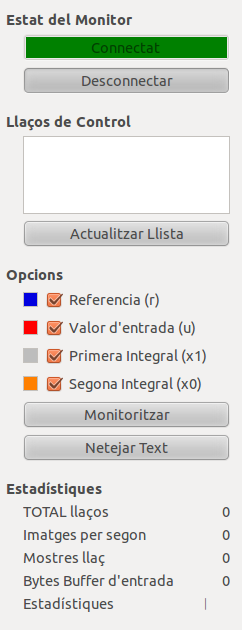
\includegraphics[scale=0.4]{idioma_ca}
		%\figuremacroW{labels_ca}{Labels en Català}{}{0.4}
	}
	\subfloat[Labels en Espanyol]{\label{idioma_es}
		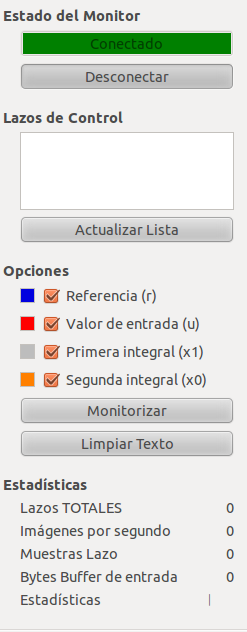
\includegraphics[scale=0.4]{idioma_es}
		%\figuremacroW{labels_es}{Labels en Espanyol}{}{0.4}
	}
	\subfloat[Labels en Anglés]{\label{idioma_en}
		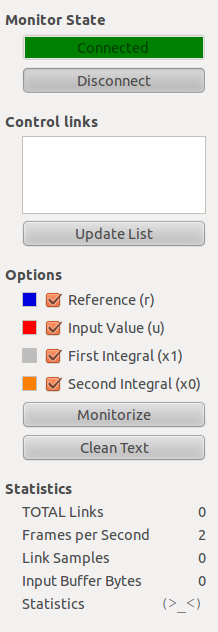
\includegraphics[scale=0.4]{idioma_en}
		%\figuremacroW{labels_en}{Labels en Anglés}{}{0.4}
	}
	\subfloat[Labels en Francés]{\label{idioma_fr}
		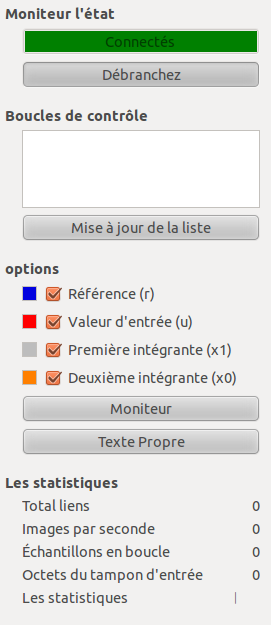
\includegraphics[scale=0.4]{idioma_fr}
		%\figuremacroW{labels_fr}{Labels en Francés}{}{0.4}
	}
	\caption{Comparació dels labels entre diferents idiomes.}
    \label{fig:comparacio_idiomes}
\end{figure}

\FloatBarrier

%====================================================================================%
% dsPIC
%====================================================================================%
\section{dsPIC}\label{lab:imp:dspic:monitor}

Aquesta secció pretén explicar les parts del codi més importants dels microcontroladors dsPIC. Tot el sistema està basat en el RTOS Erika Enterprise, així que la majoria de les funcions són tasques que són activades, o es realitzen periòdicament mitjançant alarmes.

Aquesta manera de programar permet la concurrència entre diferents tasques, el que comporta una major atenció als diferents tipus de accions que el microcontrolador ha de dur a terme.

En els microcontroladors que utilitzem aquesta concurrència es en el mateix nucli, per tant tot s'executa en serie, però aquest sistema operatiu garanteix l'execució de totes les tasques.

Tot seguit es poden veure les diferents parts més importants d'aquests programes.

%====================================================================================%
% Tasques TODO
%====================================================================================%
\subsection{Tasques en Erika}\label{lab:imp:dspic:monitor:tasks}

El RTOS Erika ens ofereix una serie d'eines per generar d'alguna manera tasques que s'executin periòdicament. En el nostre laboratori ens aprofitem d'aquesta facilitat i moltes de les funcions que fem servir en els diferents dispositius estan realitzades d'aquesta manera.

Per tal d'aconseguir això primerament s'han de declarar les tasques que el nostre Sistema Operatiu podrà executar. Per això existeix un fitxer anomenat \emph{conf.oil} en el qual hem d'avisar a RT-Druid de la creació de les tasques que necessitem, a les quals se'ls pot assignar una prioritat diferent i temps màxim d'atenció entre d'altres opcions. També es necessari indicar-li quin dispositiu volem programar, amb quin programador, quins codis formaran part del SO, i altres qüestions que podem configurar. 

Tot seguit es posa a mode d'exemple el fitxer \emph{conf.oil} necessari per programar un dispositiu que només té la tasca de supervisió (aquesta tasca enviava informació d'estat a l'ordinador via RS232).

En el codi \ref{lab:imp:dspic:monitor:tasks:oil}, es pot veure la declaració del nostre sistema indicant-li el microcontrolador que usarem, els fitxers que formaran part del codi, i finalment la declaració de la tasca \emph{TaskSupervision} amb una prioritat de valor dos (valor més alt indica major prioritat), li donem també el máxim de temps per ser executada i que volem que la administri completament el Sistema Operatiu.

Més abaix creem una alarma per poder executar aquesta tasca de manera periòdica en cas de necessitar-ho.


\begin{code_c}{Exemple de declaració d'una tasca en el fitxer conf.oil}{lab:imp:dspic:monitor:tasks:oil}
CPU mySystem {

	OS myOs {
		EE_OPT = "DEBUG";

		CPU_DATA = PIC30 {
			APP_SRC = "setup.c";
			APP_SRC = "uart_dma.c";
			APP_SRC = "e_can1.c";
			APP_SRC = "code.c";
			MULTI_STACK = FALSE;
			ICD2 = TRUE;
		};

		MCU_DATA = PIC30 {
			MODEL = PIC33FJ256MC710;
		};

		BOARD_DATA = EE_FLEX {
			USELEDS = TRUE;
		};

		
		KERNEL_TYPE = EDF { NESTED_IRQ = TRUE; TICK_TIME = "25ns";};
		
	};

	TASK TaskSupervision {
		REL_DEADLINE = "0.1s";
		PRIORITY = 2;
		STACK = SHARED;
		SCHEDULE = FULL;
	};

	COUNTER myCounter;
	
	ALARM AlarmSupervision {
		COUNTER = "myCounter";
		ACTION = ACTIVATETASK { TASK = "TaskSupervision"; };
	};
}; 
\end{code_c}

Un cop tenim ben definit l'entorn del nostre Sistema Operatiu ja només cal utilitzar les tasques dintre del programa (codis d'exemple \ref{lab:imp:dspic:monitor:tasks:interact}). Per poder posar en marxa una tasca RT-Druid ens dona la funció \emph{ActivateTask(nom de la tasca)}, amb la qual només s'executarà un cop. 

En el cas de voler activat aquesta tasca periódicament podem activar una alarma amb la funció \emph{SetRelAlarm(AlarmType AlarmID, TickType increment, TickType cycle)} en la qual li indiquem el nom de l'alarma a executar, el temps d'espera per executar-la i el temps entre cicles d'execució. Finalment si en algun moment volguessin aturar aquesta alarma cíclica només hauríem de cridar la funció \emph{CancelAlarm(AlarmType AlarmID)}.

\begin{code_c}{Codis per interactuar amb tasques}{lab:imp:dspic:monitor:tasks:interact}
// Active one execution of a task
ActivateTask(TaskSupervision);

//Data is sent to the PC every 10ms
SetRelAlarm(AlarmSupervision, 1000, 10);

// Stops the periodiciti of a task
CancelAlarm(AlarmSupervision);
\end{code_c}


%====================================================================================%
% Comunicació sèrie
%====================================================================================%
\subsection{Comunicació serie RS232}\label{lab:imp:dspic:monitor:serie}

En aquest apartat explicarem com s'ha implementat la comunicació serie per RS232 que es va dissenyar en la secció \ref{cap:dis:comSer}. Recordem que els dos dispositius capaços d'interaccionar mitjançant aquesta tecnologia són el \Monitor i el \SensorActuador, per tant s'explicaran els codis d'aquests relacionats amb la comunicació serie.

%====================================================================================%
% Recepció de senyals de control
%====================================================================================%
\subsubsection{Recepció de senyals de control}\label{lab:imp:dspic:monitor:ser:rec}

Com hem explicat en la secció anterior \ref{cap:dis:comSer}, el dispositiu \Monitor ha de ser capaç de rebre diferents instruccions del programa \DCSMonitor per tal de poder posar en marxa certes accions.

Aquestes instruccions estan numerades i les dues parts de la comunicació han de coneixer-la, per tant primer de tot en el codi del \Monitor cal declarar aquests valors:

\begin{code_c}{Declaració dels valors dels senyals de control}{lab:imp:dspic:monitor:ser:define:signals}
#define SIGNAL_STOP			1
#define SIGNAL_MONITOR		0
#define SIGNAL_PERCENT		2
#define SIGNAL_DEVICES		4
\end{code_c}

Per tal de rebre els missatges per el port sèrie RS232 es va observar el mode de funcionament de la recepció dels missatges CAN i es va utilitzar la mateixa metodologia, creant una funció que s'executés cada cop que el port sèrie s'omplís amb 8 bytes. Aquesta funció seria la encarregada de comprovar el primer dels 8 bytes del missatge, i realitza una o altre acció depenent de la taula que s'ha mostrat anteriorment \ref{tab:ids:rs232}.

Tot seguit es pot veure la funció que rep la interrupció del buffer d'entrada del port sèrie:

\begin{code_c}{Interrupció buffer del port sèrie}{lab:imp:dspic:monitor:ser:int:in:code}
// Input serial buffer interrupt
ISR2(_DMA5Interrupt) //NOTE: Disabled when IEC3bits.DMA5IE = 0;
{
	float *p_k0=(float *)&InBufferA[0];
	unsigned long id_link;

	/*Code to update received data*/
	k_updated[0]= *(p_k0);
	k_updated[1]= *(p_k0+1);

	switch (InBufferA[0])
	{
	case SIGNAL_MONITOR:

		id_link = (unsigned long) InBufferA[7]<<2;
		// Generating id's for a control plant
		ID_TO_ACTUATOR 		= CONTROL_MESSAGE 			| GENERAL_PRIORITY | id_link;
		ID_FROM_SENSOR		= GRANTED_SENSOR_MESSAGE 	| GENERAL_PRIORITY | id_link;
		ID_REFERENCE		= GENERAL_PURPOSE_MESSAGE 	| GENERAL_PRIORITY | id_link | REFERENCE_MESSAGE;
		ID_SUPERVISOR		= GENERAL_PURPOSE_MESSAGE 	| GENERAL_PRIORITY | id_link | SUPERVISOR_MESSAGE;

		// Activating filters for different message id's
		//ecan1WriteRxAcptFilter(filter, id, exide, buffer, masc)
		ecan1WriteRxAcptFilter(0x0,ID_FROM_SENSOR	,0x1,0x1,0x2);
		ecan1WriteRxAcptFilter(0x1,ID_TO_ACTUATOR	,0x1,0x2,0x2);
		ecan1WriteRxAcptFilter(0x2,ID_REFERENCE		,0x1,0x3,0x2);
		ecan1WriteRxAcptFilter(0x3,ID_SUPERVISOR	,0x1,0x4,0x2);
		CancelAlarm(AlarmSupervision);
		// Starts sending supervision messages
		SetRelAlarm(AlarmSupervision, 1000, 10);
		monitoring = 1;
		break;

	case SIGNAL_PERCENT:
		// Starts to generate useless CAN messages
		CancelAlarm(AlarmCANUseless);
		SetRelAlarm(AlarmCANUseless, 1000,101-(InBufferA[7]));
		break;

	case SIGNAL_MONITOR+SIGNAL_STOP:
		// Stops the reception of control messages
		ecan1DisableRXFilter(0x0);
		ecan1DisableRXFilter(0x1);
		ecan1DisableRXFilter(0x2);
		ecan1DisableRXFilter(0x3);
		// If is not listing devices, stops to send supervisions
		if (!listing) CancelAlarm(AlarmSupervision);
		LATBbits.LATB14 = 0;
		monitoring = 0;
		break;

	case SIGNAL_PERCENT+SIGNAL_STOP:
		// Stops the generation of usless messages
		CancelAlarm(AlarmCANUseless);
		break;

	case SIGNAL_DEVICES:
		// Activate filter 4 to put all CAN messages into buffer 5
		ecan1WriteRxAcptFilter(0x4,0x00000000,0x1,0x5,0x1);
		SetRelAlarm(AlarmSupervision, 1000, 10);
		listing = 1;
		break;

	case SIGNAL_DEVICES+SIGNAL_STOP:
		// Desactivate filter 4
		ecan1DisableRXFilter(0x4);
		// If is not monitoring devices, stops to send supervisions
		if (!monitoring) CancelAlarm(AlarmSupervision);
		LATBbits.LATB14 = 0;
		listing = 0;
		break;

	default:
		break;
	}

	IFS3bits.DMA5IF = 0; // Clear the DMA1 Interrupt Flag
}
\end{code_c}

%====================================================================================%
% Recepció de senyals de control
%====================================================================================%
\subsubsection{Enviament de dades}\label{lab:imp:dspic:monitor:ser:send}

Tant el dispositiu \Monitor com el dispositiu \SensorActuador compten amb la informació periòdica d'algun llaç de control. Aquesta informació es va emmagatzemant temporalment per enviar-les cada 10 ms al programa \DCSMonitor.

Per realitzara aquesta tasca periòdicament el \SensorActuador activa una alarma al iniciar l'execució, el \Monitor en canvi, espera a que el programa \DCSMonitor li indiqui (codi \ref{lab:imp:dspic:monitor:ser:send:alarm})

\begin{code_c}{Alarma de supervisió}{lab:imp:dspic:monitor:ser:send:alarm}
//Data is sent to the PC every 10ms
SetRelAlarm(AlarmSupervision, 1000, 10);
\end{code_c}

La informació que envien els diferents dispositius varía, així el \SensorActuador envia només 23 bytes, amb els valors del temps, referència, entrada i primera i segona integral. En canvi el \Monitor envia 71 bytes, els quals porten la mateixa informació que hem dit, però poden incloure'n més. En aquest cas afegeixen els diferents identificadors de llaç de control, existents al bus CAN.

En el codi següent es pot veure la part comuna a tots dos codis, i una part que és única del dispositiu \Monitor, en la que comprova si hi ha identificadors a la pila, per cada identificador que veu incrementa el valor del byte 22, i guarda en les següents posicions els identificadors que va trobant. Al final posa el byte 21 a 2, per indicar-li al programa \Monitor que li està enviant identificadors (codi \ref{lab:imp:dspic:monitor:ser:send:task}). 

\begin{code_c}{Tasca de Supervisió}{lab:imp:dspic:monitor:ser:send:task}
TASK(TaskSupervision)
{
	//Send_buffer_to_pc();

	static unsigned char *p_r = (unsigned char *)&r;
	static unsigned char *p_x0= (unsigned char *)&x[0];
	static unsigned char *p_x1= (unsigned char *)&x[1];
	static unsigned char *p_u = (unsigned char *)&u;

	//static unsigned long sys_time=0;

	LATBbits.LATB10 = 1; //To get time with the oscilloscope

	sys_time=GetTime();  //Get system time (EDF Scheduler)

	//Read_State();        //Before sending state, read it

	OutBuffer[0]=0x01;//header;
	OutBuffer[1]=(unsigned char)(sys_time>>24);//4th byte of unsigned long
	OutBuffer[2]=(unsigned char)(sys_time>>16);//3rd byte of unsigned long
	OutBuffer[3]=(unsigned char)(sys_time>>8); //2nd byte of unsigned long
	OutBuffer[4]=(unsigned char)sys_time;      //1st byte of unsigned long
	OutBuffer[5]=*p_r;    //4th byte of float (32bits)
	OutBuffer[6]=*(p_r+1);//3rd byte of float (32bits)
	OutBuffer[7]=*(p_r+2);//2nd byte of float (32bits)
	OutBuffer[8]=*(p_r+3);//1st byte of float (32bits)
	OutBuffer[9]=*p_x0;
	OutBuffer[10]=*(p_x0+1);
	OutBuffer[11]=*(p_x0+2);
	OutBuffer[12]=*(p_x0+3);
	OutBuffer[13]=*p_x1;
	OutBuffer[14]=*(p_x1+1);
	OutBuffer[15]=*(p_x1+2);
	OutBuffer[16]=*(p_x1+3);
	OutBuffer[17]=*p_u;
	OutBuffer[18]=*(p_u+1);
	OutBuffer[19]=*(p_u+2);
	OutBuffer[20]=*(p_u+3);


	// This is for Monitor device
	
	OutBuffer[22]=0x00;//number of devices;
	unsigned char id;
	int i = 23;
	while (get_device(&id))
	{
		OutBuffer[i++]=(unsigned char)id;   //1st byte of unsigned long
		OutBuffer[22]++;
	}
	if (OutBuffer[22] != 0x00)
		OutBuffer[21]=0x02;
	else
		OutBuffer[21]=0x00;
		
	// End extra part of Monitor device

	//Force sending data
	DMA4CONbits.CHEN  = 1;			// Re-enable DMA4 Channel
	DMA4REQbits.FORCE = 1;			// Manual mode: Kick-start the first transfer

	LATBbits.LATB10 = 0; //To get time with the oscilloscope
}
\end{code_c}

%====================================================================================%
% Comunicació CAN
%====================================================================================%
\subsection{Comunicació bus CAN}\label{lab:imp:dspic:can}

Com hem vist a la secció de disseny \ref{cap:dis:idCAN}, existeix varis tipus de missatges que poden coexistir en el bus CAN, i a més d'això aquest tipus de missatges poden pertànyer a diferents llaços de control (fins un màxim de 256).

Administrar tots aquests missatges no és una feina fàcil, per això es va haver de crear diferents regles de filtratge per facilitar aquesta tasca.

Tot seguit en aquesta secció es podrà veure com s'ha implementat aquest tipus de mascares, els diferents filtres, i l'atenció als diferents missatges que circulen per el bus CAN.

%====================================================================================%
% Creació de les màscares CAN
%====================================================================================%
\subsubsection{Creació de les màscares CAN}\label{lab:imp:dspic:monitor:can:masc}

Perquè el dispositiu \Monitor sigui capaç de capturar els diferents missatges del bus CAN, hem de crear unes màscares per poder aplicar als filtres que posteriorment creem. Aquestes màscares tenen com a objectiu, indicar quins dels bits del filtre són els que han de coincidir amb l'identificador del missatge CAN que circula per el bus, i d'aquesta manera capturar només aquestes coincidències.

Com aquest dispositiu rebrà els missatges en dos modes diferents, hem creat dos màscares noves que són les que utilitzarà en aquest laboratori, i hem deixat una mascara genèrica que fins ara era necessària, i que segons com evolucioni el programa podria ser-nos d'utilitat.

\begin{center}
	\begin{tabularx}{\linewidth}{l | l | X}
		\textbf{Num} & \textbf{Bits} & \textbf{Utilitat} \\
		\hline
		0 & \texttt{0x1FFFFFFF} & Només deixa passar els identificadors que coincideixi totalment amb el filtre \\
		\hline
		1 & \texttt{0x00000000} & Deixa passar tots els missatges, sense tenir en compte el filtre \\
		\hline
		2 & \texttt{0x1C0003FF} & Deixa passar els missatges en els que coincideixi la classe, l'id del llaç, i la subclasse amb els del filtre\\
		\hline
	\end{tabularx}
	\captionof{table}{Màscares per bus CAN}
	\label{tab:imp:dspic:monitor:mascares}
\end{center}

El codi que crea aquestes màscares es troba inclòs en la funció de configuració del dispositiu CAN (Funció \ref{lab:imp:dspic:monitor:monitoritzacio:mascares}), el qual crida a la funció \emph{ecan1Initialize()} la qual configura el dispositiu CAN, i crea dos buffers, un d'entrada i un de sortida mitjançant DMA's.

\begin{code_c}{Funció eCAN1 config}{lab:imp:dspic:monitor:monitoritzacio:mascares}
void eCAN1_config(void)
{
	//Initialize enhanced CAN bus number 1
	ecan1Initialize();

	//ecan1WriteRxAcptMask(num masc, bit masc, mide, exide)
	ecan1WriteRxAcptMask(0x0,0x1FFFFFFF, 0,0x1);
	ecan1WriteRxAcptMask(0x1,0x00000000, 0,0x1);
	ecan1WriteRxAcptMask(0x2,0x1C0003FF, 0,0x1);
}
\end{code_c}

%====================================================================================%
% Creació dels filtres CAN
%====================================================================================%
\subsubsection{Creació dels filtres CAN}\label{lab:imp:dspic:monitor:can:filtres}

Els filtres CAN ens serveixen primerament per descartar els missatges CAN que no siguin valuosos per el nostre objectiu, i per altra banda els utilitzarem per separar en diferents buffers provisionals els missatges que ens siguin d'interès.

D'aquesta manera el dispositiu \Actuador estarà interessat només en els missatges de control, per tant aquest dispositiu filtrarà aquest tipus de missatges a un buffer en concret, el qual al estar ple activarà una interrupció.
El mateix passarà amb els altres dispositius, per tant hem definit dins del codi els diferents elements que formen l'identificador, per crear els filtres més fàcilment.

\begin{code_c}{Definicions per la creació de filtres CAN}{lab:imp:dspic:monitor:constants:filtres}
// DEFINITIONS TO CREATE CAN ID'S
// id CAN : 0b 000c ccpp pppp pppp pppp ppii iiii iiss
// ccc = CLASS
// pppp pppp pppp pppp = PRIORITY
// iiii iiii = ID_PLANT
// ss = SUBCLASS

// MESSAGE SUBCLASS
#define  REFERENCE_MESSAGE 			(0)
#define  SUPERVISOR_MESSAGE 		(1)

// MESSAGE ID
#define  ID_PLANT					(1<<2)

// MESSAGE PRIORITY
#define  GENERAL_PRIORITY			(0xFFFF<<10)

// MESSAGE CLASS
#define  CONTROL_MESSAGE 			((unsigned long)0<<26)
#define  GRANTED_SENSOR_MESSAGE 	((unsigned long)1<<26)
#define  GENERAL_PURPOSE_MESSAGE 	((unsigned long)2<<26)
#define  BEST_EFFORT_SENSOR_MESSAGE ((unsigned long)3<<26)

unsigned long ID_TO_ACTUATOR 	= CONTROL_MESSAGE 			| GENERAL_PRIORITY | ID_PLANT;
unsigned long ID_FROM_SENSOR	= GRANTED_SENSOR_MESSAGE 	| GENERAL_PRIORITY | ID_PLANT;
unsigned long ID_REFERENCE		= GENERAL_PURPOSE_MESSAGE 	| GENERAL_PRIORITY | ID_PLANT | REFERENCE_MESSAGE;
unsigned long ID_SUPERVISOR		= GENERAL_PURPOSE_MESSAGE 	| GENERAL_PRIORITY | ID_PLANT | SUPERVISOR_MESSAGE;
\end{code_c}


%====================================================================================%
% Recepció de missatges CAN
%====================================================================================%
\subsubsection{Recepció de missatges CAN}\label{lab:imp:dspic:monitor:can:rx}

Un cop creades les diferents màscares i filtres dels missatges CAN, és hora de crear una funció que capturi les interrupcions generades per el bus CAN.

La implementació CAN amb la que comptem ens permet definir fins a 16 filtres diferents, i assignar-los a 16 buffers. Aquests buffers posen a 1 un bit en el moment en que estàn plens, per tant aprofitem aquest comportament per definir cadascun dels diferents missatges a un sol filtre i un sol buffer, d'aquesta manera en el moment que un dels buffers estigui ple, sabrem quin tipus de missatge és sense haver de mirar l'identificador. Pero existeix una excepció; en el cas de llistar tots els dispositius que existeixen al bus CAN. En aquest cas existeixen 2\textsuperscript{29} missatges diferents, i per tant hem de reunir-los d'alguna manera. Així doncs, tenint en compte que aquesta captura no és crítica pel control de cap llaç, crearem un filtre sense restriccions cap a un buffer. En el moment en que aquest buffer estigui plé, comprovarem l'identificador i el guardarem en una pila (més endevant explicarem més detalladament aquest funcionament).

En la taula  \ref{tab:imp:dspic:monitor:monitoritzacio:filtres} es pot veure els diferents filtres que s'han de crear, i a quin buffer estan assignats. De totes maneres, la activació o desactivació o canvi d'aquests filtres es pot realitzar en temps d'execució, pel que fa que per exemple el \Monitor els activi i desactivi a conveniència, mentre que els dispositius \Controlador i \SensorActuador no els cal modificar.

\begin{center}
	\begin{tabular}{c|l|c|c|l}
		\textbf{Num} & \textbf{Id} & \textbf{Extended} & \textbf{Buffer} & \textbf{mascara} \\
		\hline
		0 & ID\_FROM\_SENSOR & sí & 1 & \texttt{0x1C0003FF} \\
		\hline
		1 & ID\_TO\_ACTUATOR & sí & 2 & \texttt{0x1C0003FF} \\
		\hline
		2 & ID\_REFERENCE & sí & 3 & \texttt{0x1C0003FF} \\
		\hline
		3 & ID\_SUPERVISOR & sí & 4 & \texttt{0x1C0003FF} \\
		\hline
		4 & indiferent & sí & 5 & \texttt{0x00000000} \\
		\hline
	\end{tabular}
	\captionof{table}{Configuració dels filtres}
	\label{tab:imp:dspic:monitor:monitoritzacio:filtres}
\end{center}

Tenint clar a quin buffer es redireccionarà cada missatge CAN, s'ha implementat la funció d'atenció a aquestes interrupcions tenint en compte el buffer activat; com es pot veure en el codi de la funció \ref{lab:imp:dspic:monitor:can:rx:code}.

\begin{code_c}{Funcio activada per una interrupció del bus CAN}{lab:imp:dspic:monitor:can:rx:code}
/* CAN bus 1 Interrupt, ISR2 type */
ISR2(_C1Interrupt)
{
	IFS2bits.C1IF = 0; // clear interrupt flag

	// Transmission interrupt (nothing to be done but clear flag)
	if(C1INTFbits.TBIF)
    {
    	C1INTFbits.TBIF = 0;
    }

	/*Reception interrupt, different code for different filtered id's */
	if(C1INTFbits.RBIF)
	{
		LATBbits.LATB14 ^= 1;//Toggle orange led
    	/* Filter 0(ID_FROM_SENSOR):
    	 * Sensor to controller message */
    	if(C1RXFUL1bits.RXFUL1==1)
	    {
    		/* Tells rxECAN1 the buffer to pass from DMA to RAM */
	    	rx_ecan1message1.buffer=1;

	    	C1RXFUL1bits.RXFUL1=0;
		    rxECAN1(&rx_ecan1message1);
			C1INTFbits.RBIF = 0;

			/* Custom code to address Sensor message */
		    ActivateTask(TaskControllerMonitor);
	    }

		/* Filter 1(ID_TO_ACTUATOR):
		 * Controller to Actuator message */
		if(C1RXFUL1bits.RXFUL2==1)
		{
			/*Tells rxECAN1 the buffer to pass from DMA to RAM */
			rx_ecan1message2.buffer=2;

			C1RXFUL1bits.RXFUL2=0;
			rxECAN1(&rx_ecan1message2);
			C1INTFbits.RBIF = 0;

			/* Custom code to capture values from controller */
			ActivateTask(TaskActuatorMonitor);
		}

		/* Filter 2(ID_REFERENCE):
		 * Controller updated reference (supervision) */
		if(C1RXFUL1bits.RXFUL3==1)
		{
			/*Tells rxECAN1 the buffer to pass from DMA to RAM */
			rx_ecan1message3.buffer=3;

			C1RXFUL1bits.RXFUL3=0;
			rxECAN1(&rx_ecan1message3);
			C1INTFbits.RBIF = 0;

			/* Custom code to address the Controller message
			 * which updates the reference change */
			r=*(float *)(&rx_ecan1message3.data[0]);
		}

		//Filter 3(ID_SUPERVISOR): ID_SUPERVISOR
		if(C1RXFUL1bits.RXFUL4==1)
		{
			/*Tells rxECAN1 the buffer to pass from DMA to RAM */
			rx_ecan1message4.buffer=4;

			C1RXFUL1bits.RXFUL4=0;
			rxECAN1(&rx_ecan1message4);
			C1INTFbits.RBIF = 0;

			/* Custom code to address Sensor message */
			ActivateTask(TaskSensor_supervision);
		}

		//Filter 4(ALL): all messages
		if(C1RXFUL1bits.RXFUL5==1)
		{
			/*Tells rxECAN1 the buffer to pass from DMA to RAM */
			rx_ecan1message5.buffer=5;

			C1RXFUL1bits.RXFUL5=0;
			rxECAN1(&rx_ecan1message5);
			C1INTFbits.RBIF = 0;

			char id_link = (char)(rx_ecan1message5.id>>2)& 0xFF;

			/* Custom code to add an id to a list*/
			if (!search_device(id_link))
				add_device(id_link);
		}
	}
}
\end{code_c}


%====================================================================================%
% Pila de llaços de control
%====================================================================================%
\subsubsection{Pila de llaços de control}\label{lab:imp:dspic:monitor:can:stack}

Quan el \Monitor necessita llistar els diferents llaços de control del bus CAN primer ha de capturar aquests identificadors per més tard enviar-li periòdicament al programa \DCSMonitor. Per dur a terme aquesta tasca de manera modular s'ha creat un tipus d'estructura que anomenarem pila (codi \ref{lab:imp:dspic:code:stack:struct} ).
Aquesta pila és estàtica i té una mida de 30 identificadors, però per poder modificar tot això sense haver de reimplementar el codi del \Monitor s'han creat funcions tot un seguit de funcions bàsiques per tractar amb els valors continguts en ella.

\begin{code_c}{Pila d'identificadors}{lab:imp:dspic:code:stack:struct}
#define STACK_SIZE 30

struct stack{
	unsigned char ids[STACK_SIZE];
	int num;
	int max;
}stack_ids;
\end{code_c}


Tot seguit es posen els codis de tractament de la pila:

\begin{itemize}
	\item Inicialitzar \ref{lab:imp:dspic:code:stack:init}
	\item Comprovar si és plena \ref{lab:imp:dspic:code:stack:full}
	\item Buscar identificador \ref{lab:imp:dspic:code:stack:search}
	\item Afegir identificador \ref{lab:imp:dspic:code:stack:add}
	\item Treure identificador \ref{lab:imp:dspic:code:stack:get}
\end{itemize}

\begin{code_c}{Inicialitzar pila}{lab:imp:dspic:code:stack:init}
void init_devices_list()
{
	stack_ids.num = 0;
	stack_ids.max = STACK_SIZE;
}
\end{code_c}

\begin{code_c}{Comprovar si la pila és plena}{lab:imp:dspic:code:stack:full}
int stack_full()
{
	return (stack_ids.num == stack_ids.max);
}
\end{code_c}

\begin{code_c}{Buscar a la pila}{lab:imp:dspic:code:stack:search}
int search_device(unsigned char id)
{
	int i;
	for (i = 0; i < stack_ids.num; i++)
		if (stack_ids.ids[i] == id) return 1;
	return 0;
}
\end{code_c}

\begin{code_c}{Afegir a la pila}{lab:imp:dspic:code:stack:add}
int add_device(unsigned char id)
{
	if (stack_ids.num == stack_ids.max) return 0;
	stack_ids.ids[stack_ids.num] = id;
	stack_ids.num++;
	return 1;
}
\end{code_c}

\begin{code_c}{Treure de la pila}{lab:imp:dspic:code:stack:get}
int get_device(unsigned char * id)
{
	if (stack_ids.num == 0) return 0;
	*id = stack_ids.ids[stack_ids.num-1];
	stack_ids.num--;
	return 1;
}
\end{code_c}

%====================================================================================%
% Tractament de missatge ID_TO_ACTUATOR
%====================================================================================%
\subsubsection{Tractant missatges de control per l'\Actuador}\label{lab:imp:dspic:ID_TO_ACTUATOR}

Aquests missatges com s'ha explicat en la secció \ref{cap:dis:CAN:nou:CtoA}, porten amb ells el valor a aplicar a l'entrada del doble integrador. Les dades del missatge són emmagatzemades en el buffer 2, per tant primer de tot es comprova que sigui un missatge d'aquest tipus (codi \ref{lab:imp:dspic:to:actuator:rec:code}).

Aquest codi desactiva els flags del buffer que s'han activat al omplir-se, i crida a una tasca.

\begin{code_c}{Captura del missatge de control per l'\Actuador}{lab:imp:dspic:to:actuator:rec:code}
/* Filter 1(ID_TO_ACTUATOR):
 * Controller to Actuator message */
if(C1RXFUL1bits.RXFUL2==1)
{
	/*Tells rxECAN1 the buffer to pass from DMA to RAM */
	rx_ecan1message2.buffer=2;

	C1RXFUL1bits.RXFUL2=0;
	rxECAN1(&rx_ecan1message2);
	C1INTFbits.RBIF = 0;

	/* Custom code to capture values from controller */
	ActivateTask(TaskActuatorMonitor);
}
\end{code_c}


En el cas del \Monitor només necessita aquesta informació per poder enviar-la al programa \DCSMonitor perquè pugui generar les gràfiques correctament, per tant la tasca que activa només guarda aquests valors per posteriorment ser enviats (codi \ref{lab:imp:dspic:to:actuator:task:actuator:monitor:code}) per RS232.

\begin{code_c}{Tasca per capturar el valor de l'actuador}{lab:imp:dspic:to:actuator:task:actuator:monitor:code}
/* ActuatorMonitor Task */
static float *p_u = (float *)&rx_ecan1message2.data[0];
static unsigned long sys_time=0;

TASK(TaskActuatorMonitor)
{
	//sys_time=GetTime();  //Get system time (EDF Scheduler)
	u=(*p_u);
	x0=*(p_x0);//Get state x[0] from rx_ecan1_message1[0]..[3] data field
	x1=*(p_x1);//Get state x[1] from rx_ecan1_message1[4]..[7] data field
}
\end{code_c}

En canvi en el cas de l'\Actuador aquest valor l'ha d'introduir al PWM destinat a l'entrada del doble integrador (codi \ref{lab:imp:dspic:to:actuator:task:actuator:actuator:code})

\begin{code_c}{Tasca per aplicar el valor al PWM}{lab:imp:dspic:to:actuator:task:actuator:actuator:code}
/* Actuator Task */
static float *p_u = (float *)&rx_ecan1message2.data[0];

TASK(TaskActuator)
{
	u=(*p_u);

	PDC1=((*(p_u))/v_max)*0x7fff+0x3FFF;
}
\end{code_c}

%====================================================================================%
% Tractament de missatge ID_FROM_SENSOR
%====================================================================================%
\subsubsection{Tractant missatges d'estat del \Sensor per al \Controlador}\label{lab:imp:dspic:ID_FROM_SENSOR}

Els missatges d'estat contenen els valors de sortida de la primera i segona integral (capitol \ref{cap:dis:CAN:nou:StoC}). Com hem vist anteriorment (taula \ref{tab:imp:dspic:monitor:monitoritzacio:filtres}) aquests missatges estan dirigits al buffer 1, per tant al activar-se la interrupció i comprovar que aquest buffer està ple activarem la tasca Controller en el cas del dispositiu \Controlador, i la tasca ControllerMonitor en el cas del \Monitor.

Aquí es pot veure el codi que detecta aquest missatge i activa la tasca del \Monitor (codi \ref{lab:imp:dspic:from:sensor:code}):

\begin{code_c}{Captura del missatge d'estat del Sensor al Controlador}{lab:imp:dspic:from:sensor:code}
/* Filter 0(ID_FROM_SENSOR):
 * Sensor to controller message */
if(C1RXFUL1bits.RXFUL1==1)
{
	/* Tells rxECAN1 the buffer to pass from DMA to RAM */
	rx_ecan1message1.buffer=1;

	C1RXFUL1bits.RXFUL1=0;
    rxECAN1(&rx_ecan1message1);
	C1INTFbits.RBIF = 0;

	/* Custom code to address Sensor message */
    ActivateTask(TaskControllerMonitor);
}
\end{code_c}

Per tant, el dispositiu \Monitor només captura els valors de l'estat del doble integrador (codi \ref{lab:imp:dspic:from:sensor:code:cap:mon}).

\begin{code_c}{Tasca per capturar el valor d'estat del control}{lab:imp:dspic:from:sensor:code:cap:mon}
static float *p_x0 = (float *)&rx_ecan1message1.data[0];
static float *p_x1 = (float *)&rx_ecan1message1.data[4];
static float x0=0;
static float x1=0;
TASK(TaskControllerMonitor)
{
	x0=*(p_x0);//Get state x[0] from rx_ecan1_message1[0]..[3] data field
	x1=*(p_x1);//Get state x[1] from rx_ecan1_message1[4]..[7] data field
	x[0] = x0;
	x[1] = x1;
}
\end{code_c}

Mentre que el dispositiu \Controlador utilitza aquests valors per fer els calculs del control (codi \ref{lab:imp:dspic:from:sensor:code:calc:con}); puntualitzem que en aquest cas el control no és bo. Un cop ha determinat el valor d'entrada per el doble integrador, activa una funció per enviar aquest valor en un missatge CAN (funció \ref{lab:imp:dspic:from:sensor:code:send:cont}).

\begin{code_c}{Tasca per fer els calculs del control}{lab:imp:dspic:from:sensor:code:calc:con}
static float Nu =0.0;
static float Nx[2] ={1.0,0.0};
static float k[2]={0.9834 ,  -0.8931};
static float x_hat[2]={0,0};
static float u_ss=0;

static float *p_x0 = (float *)&rx_ecan1message1.data[0];
static float *p_x1 = (float *)&rx_ecan1message1.data[4];
static float x0=0;
static float x1=0;
TASK(TaskController)
{
	x0=*(p_x0);//Get state x[0] from rx_ecan1_message1[0]..[3] data field
	x1=*(p_x1);//Get state x[1] from rx_ecan1_message1[4]..[7] data field

	x_hat[0]=x0-r*Nx[0];//Nx, Nu matrices needed for regulation purposes
	x_hat[1]=x1-r*Nx[1];
	u_ss=r*Nu;

	u=-k[0]*x_hat[0]-k[1]*x_hat[1]+u_ss;

	/* Check for saturation */
	if (u>v_max/2) u=v_max/2;
	if (u<-v_max/2) u=-v_max/2;

	Send_Controller2Actuator_message(&u);//identifier=ID_PLANT+1
}
\end{code_c}

Aquesta funció segueix el patró explicat en l'apartat \ref{cap:dis:CAN:nou:CtoA}, el qual només conté el valor a introduir al doble integrador.

\begin{code_c}{Funció per enviar senyal de control per bus CAN}{lab:imp:dspic:from:sensor:code:send:cont}
static unsigned char *p_data= NULL;
void Send_Controller2Actuator_message(float *data)
{
	p_data=(unsigned char *)data;
	C1CTRL1bits.ABAT = 1;
	while(C1TR01CONbits.TXREQ0){};

	tx_ecan1message.buffer=0;//Buffer number
	tx_ecan1message.frame_type=1;//0->Std Id, 1->Ext Id

	tx_ecan1message.id=ID_TO_ACTUATOR;//Identifier;
	tx_ecan1message.message_type=0;//0->Normal, 1->Remote Transmit
	tx_ecan1message.data_length=4;//Length of data (0 to 8 bytes)
	tx_ecan1message.data[0]= *p_data;
	tx_ecan1message.data[1]=*(p_data+1);
	tx_ecan1message.data[2]=*(p_data+2);
	tx_ecan1message.data[3]=*(p_data+3);

	ecan1SendMessage(&tx_ecan1message);

	while(C1TR01CONbits.TXREQ0){};
}
\end{code_c}


%====================================================================================%
% Tractament de missatge ID_REFERENCE
%====================================================================================%
\subsubsection{Tractant missatges de canvi de referencia}\label{lab:imp:dspic:ID_REFERENCE}

Els missatges de canvi de referencia són únicament indicatius per poder dibuixar la gràfica correctament (explicat en la secció \ref{cap:dis:CAN:nou:referencia}). Estan referenciats al buffer 3, i només porten el valor de referencia actual, per tant tant el \SensorActuador com el \Monitor executen el mateix codi, que detecta el tipus de missatge, i guarda el valor de referencia (codi \ref{lab:imp:dspic:reference:code}).


\begin{code_c}{Captura del missatge de canvi de referencia}{lab:imp:dspic:reference:code}
/* Filter 2(ID_REFERENCE):
 * Controller updated reference (supervision) */
if(C1RXFUL1bits.RXFUL3==1)
{
	/*Tells rxECAN1 the buffer to pass from DMA to RAM */
	rx_ecan1message3.buffer=3;

	C1RXFUL1bits.RXFUL3=0;
	rxECAN1(&rx_ecan1message3);
	C1INTFbits.RBIF = 0;

	/* Custom code to address the Controller message
	 * which updates the reference change */
	r=*(float *)(&rx_ecan1message3.data[0]);
}
\end{code_c}

%====================================================================================%
% Tractament de missatge ID_SUPERVISOR
%====================================================================================%
\subsubsection{Tractant missatges d'estat del \Sensor per al \Supervisor}\label{lab:imp:dspic:ID_SUPERVISOR}

Aquest missatge té exactament el mateix format que l'anterior \emph{missatge d'estat del \Sensor al \Controlador} però només té com a destincació el dispositiu \Monitor, per tant farà exactament el mateix que el codi vist anteriorment, però es veu activat per un filtre diferent, i es guarda en el buffer 4 (codi \ref{lab:imp:dspic:supervisor:code}).

\begin{code_c}{Captura del missatge d'estat del Sensor al Supervisor}{lab:imp:dspic:supervisor:code}
//Filter 3(ID_SUPERVISOR): ID_SUPERVISOR
if(C1RXFUL1bits.RXFUL4==1)
{
	/*Tells rxECAN1 the buffer to pass from DMA to RAM */
	rx_ecan1message4.buffer=4;

	C1RXFUL1bits.RXFUL4=0;
	rxECAN1(&rx_ecan1message4);
	C1INTFbits.RBIF = 0;

	/* Custom code to address Sensor message */
	ActivateTask(TaskSensor_supervision);
}
\end{code_c}

I aquest és el codi de la tasca que emmagatzema els valors de sortida del doble integrador (codi \ref{lab:imp:dspic:supervisor:sensor:code}).

\begin{code_c}{Tasca que emmagatzema els valors d'estat del Sensor}{lab:imp:dspic:supervisor:sensor:code}
static float *p2_x0 = (float *)&rx_ecan1message4.data[0];
static float *p2_x1 = (float *)&rx_ecan1message4.data[4];
TASK(TaskSensor_supervision)
{
	x0=*(p2_x0);//Get state x[0] from rx_ecan1_message4[0]..[3] data field
	x1=*(p2_x1);//Get state x[1] from rx_ecan1_message4[4]..[7] data field
	x[0] = x0;
	x[1] = x1;
}
\end{code_c}

%====================================================================================%
% Tractament de tots els missatges
%====================================================================================%
\subsubsection{Tractant la resta dels missatges}\label{lab:imp:dspic:ALL_ID}

Aquest tipus de tractament només l'efectua el dispositiu \Monitor, i és activat només quan necessita llistar tots els dispositius que existeixen al bus CAN. El motiu que sigui activat és perquè el nombre de dispositius que pot arribar a haver al bus és molt elevat, per tant ens interessa deixar temps per capturar els missatges del control d'un llaç.

Tots els missatges que no compleixin els altres filtres aniran al buffer 5, i per tant un cop activada la interrupció i comprovat que el buffer activat és aquest agafem l'identificador de llaç de control (que són els 8 bits començant per el tercer de la dreta; explicat en la secció \ref{cap:dis:idCAN}).

Tot seguit abans d'emmagatzemar el seu valor, comprovarem que la pila no estigui plena (la pila esta explicada en la secció \ref{lab:imp:dspic:monitor:can:stack}), i que aquest identificador no hi sigui ja, un cop comprovat l'afegirem (codi \ref{lab:imp:dspic:all:code}).

Posteriorment amb la tasca periòdica de supervisió, els identificadors apilats seran enviats al programa \DCSMonitor i la pila tornarà a estar buida.

\begin{code_c}{Captura de la resta de missatges}{lab:imp:dspic:all:code}
//Filter 4(ALL): all messages
if(C1RXFUL1bits.RXFUL5==1)
{
	/*Tells rxECAN1 the buffer to pass from DMA to RAM */
	rx_ecan1message5.buffer=5;

	C1RXFUL1bits.RXFUL5=0;
	rxECAN1(&rx_ecan1message5);
	C1INTFbits.RBIF = 0;

	char id_link = (char)(rx_ecan1message5.id>>2)& 0xFF;

	/* Custom code to add an id to a list*/
	if (!stack_full() && !search_device(id_link))
		add_device(id_link);
}
\end{code_c}

%====================================================================================%
% Monitorització d'un llaç de control
%====================================================================================%
\subsubsection{Monitorització d'un llaç de control}\label{lab:imp:dspic:monitor:monitoritzacio}

Perquè el dispositiu \Monitor sigui capaç de rebre tots els missatges CAN d'un llaç determinat, el que fem es generar els quatre identificadors dels missatges que necessitem rebre a partir del numero de llaç de control que ens envia el programa \DCSMonitor. Com hem vist en la secció anterior ( capítol \ref{cap:dis:comSer:monitor}) aquest valor ve en l'ultim byte del missatge sèrie. Per tant agafem aquest identificador i el desplacem dos bits a l'esquerra perquè quedi en la posició correcte.

Un cop tenim l'identificador bé, generem mitjançant una OR bit a bit tots els elements que formen l'identificador; els quals ja estan ben posicionats (Codi \ref{lab:imp:dspic:monitor:constants:filtres}). I creem els filtres per rebre els missatges d'aquest llaç.

\begin{code_c}{Creant filtres per monitoritzar un llaç de control}{lab:imp:dspic:monitor:monitoritzacio:filtres}
id_link = (unsigned long) InBufferA[7]<<2;
// Generating id's for a control plant
ID_TO_ACTUATOR 		= CONTROL_MESSAGE 			| GENERAL_PRIORITY | id_link;
ID_FROM_SENSOR		= GRANTED_SENSOR_MESSAGE 	| GENERAL_PRIORITY | id_link;
ID_REFERENCE		= GENERAL_PURPOSE_MESSAGE 	| GENERAL_PRIORITY | id_link | REFERENCE_MESSAGE;
ID_SUPERVISOR		= GENERAL_PURPOSE_MESSAGE 	| GENERAL_PRIORITY | id_link | SUPERVISOR_MESSAGE;

// Activating filters for different message id's
//ecan1WriteRxAcptFilter(filter, id, exide, buffer, masc)
ecan1WriteRxAcptFilter(0x0,ID_FROM_SENSOR	,0x1,0x1,0x2);
ecan1WriteRxAcptFilter(0x1,ID_TO_ACTUATOR	,0x1,0x2,0x2);
ecan1WriteRxAcptFilter(0x2,ID_REFERENCE		,0x1,0x3,0x2);
ecan1WriteRxAcptFilter(0x3,ID_SUPERVISOR	,0x1,0x4,0x2);
CancelAlarm(AlarmSupervision);
// Starts sending supervision messages
SetRelAlarm(AlarmSupervision, 1000, 10);
monitoring = 1;
\end{code_c}


%====================================================================================%
% Conclusions
%====================================================================================%
\section{Conclusions}\label{cap:imp:conc}

En aquest punt ja s'ha finalitzat tota la part de programació dels diferents dispositius i del programa d'ordinador \DCSMonitor. 

Primerament hem pogut veure quins són els passos exactes per el disseny d'una interfície mitjançant QT, i quins són els resultats que d'ell s'en deriven.

Hem vist com un programa en llenguatge \Python pot tractar amb el port serie, com s'obre aquest tipus de dispositiu, i com s'interactua amb ell per rebre i enviar missatges als perifèrics que hi hagi connectats. Després hem vist com a partir dels valors rebuts per el \Monitor podíem generar les imatges en temps real, activant un parell de tasques periòdiques que ven compenetrades aconsegueixen crear unes gràfiques que semblen en moviment. I com en qualsevol moment podem obtenir una captura d'aquesta gràfica en varis formats (.pdf, .eps, .png, .emf...). I finalment per la part del programa d'ordinador hem vist com generar els fitxers de traducció per aconseguir varis idiomes en el programa, canviant aquest idioma en temps d'execució.

Per la part dels dispositius del llaç de control hem vist com s'utilitzen les funcions del Sistema Operatiu en Temps Real Erika; com es creen tasques periòdiques, com s'activen de noves i com s'aturen,  com es creen mascares CAN, la creació de filtres i l'assignació de diferents buffers als missatges del bus CAN, que fer amb els diferents missatges que ens arriben, i com generar-ne de nous.

Ara només queda fer els càlculs del temps que hem dedicat a tot, i realitzar un anàlisi econòmic del conjunt, tot això en el següent capítol.

	

% this file is called up by thesis.tex
% content in this file will be fed into the main document

\chapter{Anàlisi econòmic}\label{cap:eco} % top level followed by section, subsection


% ----------------------- paths to graphics ------------------------

% change according to folder and file names
\ifpdf
    \graphicspath{{7_economic_analysis/figures/PNG/}{7_economic_analysis/figures/PDF/}{7_economic_analysis/figures/}}
\else
    \graphicspath{{7_economic_analysis/figures/EPS/}{7_economic_analysis/figures/}}
\fi


% ----------------------- contents from here ------------------------

En aquest capítol mostrem un desglos del preu que ha comportat aquest projecte, separant la part de materials necessaris per l'execució dels experiments de laboratori, i la part d'hores dedicades a cada una de les fases del projecte segons el tipus de personal necessari per dur la feina.

%====================================================================================%
% Material
%====================================================================================%
\section{Material}\label{cap:eco:mat}

Tot el material necessari per dur a terme el projecte, es bàsicament el material que es necessita per elaborar un laboratori de Sistemes Distribuïts de Control com el que hem realitzat, en el que existeixen dos grups de laboratori i un professor.
Cada un d'els grups de laboratori necessita per tant dues plaques \FLEX per la elaboració del control, i el professor en necessita una que faci de \Monitor. Com realment no existeixen alumnes no necessitàvem dos ordinadors per els grups ja que amb un ordinador connectat al dispositiu \Monitor ja podíem realitzar totes les lectures.

També era necessari un programador per poder programar els diferents dispositius, els alimentadors (que fent ponts entre les plaques només ens han calgut un parell), un convertidor de RS232 a USB ja que l'ordinador portàtil no comptava amb aquest port, i el material d'oficina que hem anat necessitant per prendre apunts, imprimir material didàctic, o realitzar els \LiveCD necessaris.

A continuació es pot veure desglossat el preu de tot el material mencionat (taula \ref{tab:costs:mat}).

\begin{table}[ht!]
	\begin{tabularx}{\linewidth}{l | X | l | l | l}
		%%%%%%%%%%%%%%%%%%%%%%%%%%%%%%%%%%%%%%%%%%%%%%%%%%%%%%%%%%%%%%%%%%%%%%%
%%                                                                  %%
%%  This is a LaTeX2e table fragment exported from Gnumeric.        %%
%%                                                                  %%
%%%%%%%%%%%%%%%%%%%%%%%%%%%%%%%%%%%%%%%%%%%%%%%%%%%%%%%%%%%%%%%%%%%%%%
Rol 	&Euros/hora\\
Enginyer de Software	&30\\
Enginyer Industrial	&25\\
Director de Projecte	&60\\
Becari	&15\\

\textbf{Material}	&\textbf{descripció}	&\textbf{preu un.}	&\textbf{unitats}	&\textbf{preu}\\
\hline
\hline
Placa FLEX	&Placa de prototipat de la casa \FLEX	&119	&5	&595\\
\hline
Modul CAN	&Circuit amb transceptor CAN	&8	&5	&40\\
\hline
Modul RS232	&Circuit amb codificador RS232	&9	&1	&9\\
\hline
ICD3	&Programador Mplab de la casa \Microchip	&148	&1,00	&148\\
\hline
Ordinador portatil	&Portatil estandart	&399	&1	&399\\
\hline
Alimentadors	&Alimentador 9VDC 500mA	&12	&2	&24\\
\hline
Convertidor RS232	&Convertidor de estandart RS232 a USB	&9	&1	&9\\
\hline
Cables varis	&(cables per bus CAN, cables alimentació...)	&35	&1	&35\\
\hline
Material oficina	&(impresions, dvd's, cd's, fulls...)	&50	&1	&50\\
\hline
\hline
TOTAL	&	&	&	&1309\\
\hline
	\end{tabularx}
	\caption[Preu del material necessari]{Desglos del preu de tot el material empleat}
	\label{tab:costs:mat}
\end{table}


%====================================================================================%
% Ma d'obra
%====================================================================================%
\section{Ma d'obra}\label{cap:eco:hora}


Aquest es un dels aspectes més importants a l'hora de fer el calcul de preus del projecte, ja que en aquest cas s'emporta el 90\% del pressupost total del projecte.

\begin{wraptable}{r}{0.5\textwidth}

%\begin{table}[ht!]
\begin{center}
	\begin{tabular}{|| l | c ||}
		%%%%%%%%%%%%%%%%%%%%%%%%%%%%%%%%%%%%%%%%%%%%%%%%%%%%%%%%%%%%%%%%%%%%%%%
%%                                                                  %%
%%  This is a LaTeX2e table fragment exported from Gnumeric.        %%
%%                                                                  %%
%%%%%%%%%%%%%%%%%%%%%%%%%%%%%%%%%%%%%%%%%%%%%%%%%%%%%%%%%%%%%%%%%%%%%%
Rol 	&Euros/hora\\
Enginyer de Software	&30\\
Enginyer Industrial	&25\\
Director de Projecte	&60\\
Becari	&15\\

\hline
\textbf{Rol} 	&\textbf{Preu}\\
\hline
\hline
Enginyer de Software	&30\\
\hline
Enginyer Industrial	&25\\
\hline
Director de Projecte	&60\\
\hline
Becari	&15\\
\hline
	\end{tabular}
\end{center}
	\caption[Preus hora de cada rol]{Preu de cada rol en Euros/hora}
	\label{tab:cost:hour}
%\end{table}

\end{wraptable}

Per fer aquest calcul s'ha estimat el preu de la ma d'obra de diferents rols que s'han tocat durant el projecte, per exemple l'Enginyer de Software que ha realitzat tots els codis relacionats amb interfícies, programes, disseny d'aquests, etc. L'enginyer Industrial que s'ha encarregat dels diferents protocols de comunicació, les connexions elèctriques i el disseny del laboratori físic. El director de projecte, que ha planificat els temps d'entrega, els canvis del diagrama de Gantt, i ha fet les reunions periòdiques per controlar el bon funcionament de tot. I el becari que ha fet les proves dels sistemes, documentat l'us del laboratori i de part del \LiveCD.

Per tant es posa una taula amb els preus de cada un dels diferents rols (taula \ref{tab:cost:hour}), i tot seguit un desglos dels dies dedicats a cada una de les tasques, el seu equivalent en hores, el percentatge d'elaboració d'aquestes feines per rol, i finalment el preu resultant de fer els calculs (taula \ref{tab:costs}).



Tota la feina indicada en aquesta taula es pot contrastar en el diagrama de Gantt mostrat en el primer capitol (Introducció, \ref{cap:int}) en l'apartat de planificació (secció \ref{cap:int:plan}).


\begin{table}[ht!]
	\begin{tabular}{l | r r r r | r | r | r}
		%%%%%%%%%%%%%%%%%%%%%%%%%%%%%%%%%%%%%%%%%%%%%%%%%%%%%%%%%%%%%%%%%%%%%%%
%%                                                                  %%
%%  This is a LaTeX2e table fragment exported from Gnumeric.        %%
%%                                                                  %%
%%%%%%%%%%%%%%%%%%%%%%%%%%%%%%%%%%%%%%%%%%%%%%%%%%%%%%%%%%%%%%%%%%%%%%
&E.S.	&E.C.	&P.M.	&Bec.	&dies	&hores	&Euros\\
Estudi General	&50	&50	&0	&0	&7,00	&24,50	&673,75\\
Planificar Projecte	&25	&25	&50	&0	&1,00	&3,50	&153,12\\
Laboratori Actual	&35	&60	&0	&10	&19,00	&66,50	&1.795,50\\
Preparar codis lliures	&70	&30	&0	&0	&12,40	&43,40	&1.236,90\\
Ampliaci� del laboratori	&50	&50	&0	&0	&53,40	&186,90	&5.139,75\\
Preparar Live CD	&80	&0	&0	&20	&14,00	&49,00	&1.323,00\\
Realitzar Guies	&80	&0	&0	&20	&9,40	&32,90	&888,30\\
Preparar Informe Previ	&50	&45	&5	&0	&7,00	&24,50	&716,62\\
Preparar Mem�ria	&49	&49	&2	&0	&15,00	&52,50	&1.477,88\\
Preparar Defensa	&50	&40	&5	&0	&7,00	&24,50	&686,00\\
Reuninons peri�diques	&25	&25	&50	&0	&9,00	&31,50	&1.378,12\\
TOTAL	&	&	&	&	&154,20	&539,70	&14.090,83\\

\textbf{Feina} &\textbf{E.S.}	&\textbf{E.I.}	&\textbf{P.M.}	&\textbf{Bec.}	&\textbf{dies}	&\textbf{hores}	&\textbf{Euros}\\
\hline
\hline
Estudi General	&50	&50	&0	&0	&7,00	&24,50	&673,75\\
\hline
Planificar Projecte	&25	&25	&50	&0	&1,00	&3,50	&153,12\\
\hline
Laboratori Actual	&35	&60	&0	&10	&19,00	&66,50	&1.795,50\\
\hline
Preparar codis lliures	&70	&30	&0	&0	&12,40	&43,40	&1.236,90\\
\hline
Ampliació del laboratori	&50	&50	&0	&0	&53,40	&186,90	&5.139,75\\
\hline
Preparar Live CD	&80	&0	&0	&20	&14,00	&49,00	&1.323,00\\
\hline
Realitzar Guies	&80	&0	&0	&20	&9,40	&32,90	&888,30\\
\hline
Preparar Informe Previ	&50	&45	&5	&0	&7,00	&24,50	&716,62\\
\hline
Preparar Memória	&49	&49	&2	&0	&15,00	&52,50	&1.477,88\\
\hline
Preparar Defensa	&50	&40	&5	&0	&7,00	&24,50	&686,00\\
\hline
Reuninons periódiques	&25	&25	&50	&0	&9,00	&31,50	&1.378,12\\
\hline
\hline
\textbf{TOTAL}	&	&	&	&	&\textbf{154,20}	&\textbf{539,70}	&\textbf{14.090,83}\\
\hline
	\end{tabular}
	\caption[Desglos del preu de la ma d'obra]{Desglos del preu de la ma d'obra, amb el percentatge de dedicació per rol}
	\label{tab:costs}
\end{table}

Tot seguit es pot observar una gràfica de pastís (figura \ref{economic_2}) que s'ha creat per veure visualment com s'ha distribuït la inversió de capital en la ma d'obra segons la feina que s'ha realitzat. Com era d'esperar una gran part del preu del projecte recau sobre l'elaboració de l'ampliació del nou laboratori, i la preparació anterior amb el laboratori actual, que ens va servir per entendre els Sistemes Distribuïts de Control.

\figuremacro{economic_2}{Distribució del preu segons la feina}{}


%\begin{wraptable}{r}{0.7\textwidth}

\begin{table}[ht!]
\begin{center}
	\begin{tabular}{|| l | r | r ||}
		%%%%%%%%%%%%%%%%%%%%%%%%%%%%%%%%%%%%%%%%%%%%%%%%%%%%%%%%%%%%%%%%%%%%%%%
%%                                                                  %%
%%  This is a LaTeX2e table fragment exported from Gnumeric.        %%
%%                                                                  %%
%%%%%%%%%%%%%%%%%%%%%%%%%%%%%%%%%%%%%%%%%%%%%%%%%%%%%%%%%%%%%%%%%%%%%%
Rol 	&hores	&percentatge\\
Enginyer de Software	&283,85	&53\%\\
Enginyer Industrial	&213,92	&40\%\\
Director de Projecte	&21	&4\%\\
Becari	&23,03	&4\%\\

\hline
\textbf{Rol} 	&\textbf{hores}	&\textbf{percentatge}\\
\hline
\hline
Enginyer de Software	&283,85	&53\%\\
\hline
Enginyer Industrial	&213,92	&40\%\\
\hline
Director de Projecte	&21,00	&4\%\\
\hline
Becari	&23,03	&4\%\\
\hline
	\end{tabular}
	\end{center}
	\caption[Hores dedicades per rol]{Hores dedicades al projecte per rol, i els seus percentatges}
	\label{tab:hores:rol}
\end{table}

%\end{wraptable}

També és important veure quin es el percentatge d'hores que li ha dedicat cada rol al projecte, i amb la taula \ref{tab:hores:rol} podem veure que l'Enginyer de Software i l'Enginyer Industrial són els que més hores han dedicat al projecte, donant una expectativa positiva envers el resultat del projecte.

\figuremacroW{hores}{Percentatge d'hores dedicades al projecte per rol}{}{0.6}




% this file is called up by thesis.tex
% content in this file will be fed into the main document

\chapter{Conclusions}\label{cap:conc} % top level followed by section, subsection


% ----------------------- paths to graphics ------------------------

% change according to folder and file names
\ifpdf
    \graphicspath{{8_conclusions/figures/PNG/}{8_conclusions/figures/PDF/}{8_conclusions/figures/}}
\else
    \graphicspath{{8_conclusions/figures/EPS/}{8_conclusions/figures/}}
\fi

% ----------------------- contents from here ------------------------

Amb aquest projecte hem pogut aproximar-nos als Sistemes Distribuïts de Control, i veure els problemes que aquests sistemes arrosseguen. Al principi podia ser una mica desconcertant, però un cop ens hi endinsem les coses comencen a agafar un cert sentit i es comencen a veure d'una altre manera.

En el projecte finalment hem pogut complir tots els requisits plantejats des de bon principi.

Hem pogut agafar i entendre tot el codi del laboratori actual (secció \ref{cap:dis:resum}), per d'aquesta manera crear tot l'entorn de codi lliure, el receptor dels missatges que existia anteriorment era un programa per Matlab, el qual necessitava una llicencia per ser executat, així que amb la creació del nou programa \DCSMonitor hem pogut resoldre aquest problema, ja que ara no es necessari comptar amb aquesta llicencia (secció \ref{cap:imp:dcs}).

Hem dissenyat l'entorn de laboratori d'un Sistema Distribuït de Control real, en el qual tots els dispositius comparteixen realment el mateix bus CAN, i d'aquesta manera els alumnes poden aprendre en un entorn conflictiu real (\ref{diss:nou}). 

Per dissenyar aquest laboratori hem hagut d'organitzar els diferents identificadors que hi ha permesos al protocol CAN, de manera que existeixi una jerarquia de prioritats entre els missatges CAN, que una part pugui identificar l'identificador del llaç de control, i una altra quin tipus de missatge és (secció \ref{cap:dis:idCAN}). Tot això s'ha dissenyat seguint aquests requisits, i finalment els identificadors tenen una estructura totalment ben definida.

Aquest nou laboratori ha comportat la creació d'un nou programa per ordinador; el qual hem anomenat \DCSMonitor; i que hem dissenyat per complir tots els objectius que es van plantejar. 

D'aquesta manera hem estudiat i creat tot el codi necessari perquè aquest programa fos capaç de comunicar-se a traves del port serie via RS232 a una placa \FLEX (secció \ref{cap:imp:com:serie}) per tal de: demanar un llistat de tots els llaços de control existents al bus CAN (secció \ref{cap:imp:com:serie:send:devices}), demanar-li que carregués el bus de manera que els llaços de control es veiessin amb problemes reals (secció \ref{cap:imp:com:serie:send:sat}), demanar-li totes les dades de l'estat d'un llaç de control i d'aquesta manera poder avaluar la bondat del control de cada grup del laboratori (secció \ref{cap:imp:com:serie:send:monit}). I tot això mantenint la compatibilitat del laboratori antic, creant dos modes d'execució, un en el que es totalment compatible amb les plaques \FLEX de l'antic laboratori i on cada alumne pot avaluar el seu control, i un mode d'execució en el que intervé un dispositiu nou que anomenem \Monitor, amb el que es poden fer totes les accions anteriorment comentades.

Una peculiaritat de la comunicació serie que s'ha dissenyat es que s'ha realitzat de manera que pugui ser fàcilment ampliable i reutilitzable per tal d'afegir més opcions per al \Monitor o per el programa \DCSMonitor.

Amb les dades rebudes d'un llaç de control connectat al programa, o monitoritzat per un dispositiu \Monitor, hem fet que el programa \DCSMonitor sigui capaç de generar unes gràfiques en temps real amb els valors del control de: referència, valor d'entrada del doble integrador i valors de la primera i segona integral. A més aquests plots poden ser trets de la gràfica individualment (secció \ref{cap:imp:gen:graph}).

Les gràfiques en temps real també poden ser exportades a diferents tipus d'imatge, entre d'elles imatges vectorials, molt interessants per afegir en documents o articles (secció \ref{cap:imp:exp:graph}).

Un atre dels requisits del projecte era que el programa fos multilingüe, i ho hem complert creant l'entorn disponible en català, castellà, anglès i francès (secció \ref{cap:imp:idi}). A més hem utilitzat una metodologia de programació modular que ens permet fàcilment afegir tots els idiomes que vulguem. 

A part del programa d'ordinador \DCSMonitor, també calia crear un dispositiu que pogués monitoritzar els llaços de control que es trobessin al bus CAN (dispositiu que hem anomenat \Monitor). Per tal s'ha dissenyat el sistema de recepció de missatges per RS232 del programa \DCSMonitor, activant interrupcions i comprovant quin tipus de acció es volia portar a terme, i posant en marxa diferents tasques dependents d'això (secció \ref{lab:imp:dspic:monitor:ser:rec}).

Els dispositius que ja existien en el laboratori actual s'han mantingut totalment compatibles, i s'els ha afegit el necessari per poder compartir el bus CAN sense conflictes, creant l'estructura d'identificadors de manera modular, i havent de incloure únicament el numero de grup al que pertanyen (veure codi \ref{lab:imp:dspic:monitor:constants:filtres}).

Sobre les guies, s'ha preparat una guia de laboratori per posar l'entorn de laboratori necessari per poder executar les diferents pràctiques que des de la universitat s'imparteixen (apèndix \ref{cap:lab_gui}).

També s'ha creat un \LiveCD amb un Linux \Ubuntu, amb tot el codi necessari preparat per ser arrencat i provat (el pes de tot el sistema amb \Eclipse i \MplabX inclosos han fet que el pes total del sistema sigui de 1,4GB el que ha comportat que el \LiveCD s'hagi de gravar en un DVD o en un llapis de memòria). Gracies a aquest DVD només logejar-nos podem programar el llaç de control, i començar a fer les lectures. I la guia d'aquest CD que ens explica pas a pas com poder fer una instal·lació de l'entorn en un ordinador o en una màquina virtual, i després com utilitzar-lo tant en l'entorn instal·lat com des de el \LiveCD (apèndix \ref{cap:cd_gui}).

Per tant un cop finalitzat han estat complerts tots els requisits proposats en un principi, quedant constància de manera desglossada al llarg de tota la memòria. 

Cal destacar que l'entrega d'aquest projecte no tanca aquest laboratori, ja que el disseny que s'ha realitzat durant el projecte ha estat encaminat cap al doble integrador, però s'ha programat l'entorn, i s'han pensat tots els identificadors i missatges de manera que pugui ser ampliat per atendre altre tipus de controls, realitzar diferents accions des de l'ordinador, deixant espai suficient perquè la comunicació entre el programa \DCSMonitor i el dispositiu \Monitor tinguin una gran varietat de senyals diferents i es pugui modificar el laboratori de varies maneres.
 
\subsection{Treball futur}

En el transcurs del projecte han anat apareixen diverses funcions que podien ampliar el projecte però quedaven fora de l'abast d'aquest, així que posteriorment a l'entrega d'aquest projecte encara es poden realitzar aquestes ampliacions i/o millores:

\begin{enumerate}
	\item Ampliar el nombre d'idiomes en el que està traduït el programa per l'ordinador.
	\item Traduir les guies a altres idiomes.
	\item Que el programa \DCSMonitor sigui capaç de mostrar les gràfiques de més d'un llaç de control al mateix temps.
	\item Que el dispositiu \Monitor del microcontrolador sigui capaç d'estimar el percentatge de saturació del bus CAN, i d'aquesta manera poder enviar aquesta informació al programa \DCSMonitor.
	\item Crear el codi necessari perquè els missatges CAN no provoquin interrupcions, sinó que en tot moment es faci un pooling controlat.
	\item Mirar de programar el microcontrolador amb una eina més senzilla i menys pesada que el \MplabX, el qual actualment només s'utilitza per aquest fi.
	\item Reduir la mida de la imatge del laboratori perquè càpiga en un CD.
	\item Utilitzar les tres màscares CAN disponibles en els microcontroladors.
	\item En el programa \DCSMonitor separar en diferents procesos l'adquisició de dades del port serie i el dibuix de la gràfica.
	\item Organitzar de manera eficient els textos per traduir del programa \DCSMonitor
\end{enumerate}


% ---------------------------------------------------------------------------
%: ----------------------- end of thesis sub-document ------------------------
% ---------------------------------------------------------------------------



 








%\include{7/discussion}               % discussion of results

%\include{8/materials_methods}        % description of lab methods




% --------------------------------------------------------------
%:                  BACK MATTER: appendices, refs,..
% --------------------------------------------------------------

% the back matter: appendix and references close the thesis
\appendix
%%==================================================================%%
%% Author : Perelló Nieto, Miquel                                   %%
%% Version: 1.0, 04/11/2011                                         %%
%%                                                                  %%
%% Memoria del Projecte de Final de Carrera                         %%
%% Disseny del laboratori                                           %%
%%==================================================================%%

\chapter{Guia del laboratori}\label{cap:lab_gui}


% the code below specifies where the figures are stored
\ifpdf
    \graphicspath{{5_laboratory_guide/figures/PNG/}{5_laboratory_guide/figures/PDF/}{5_laboratory_guide/figures/}}
\else
    \graphicspath{{5_laboratory_guide/figures/EPS/}{5_laboratory_guide/figures/}}
\fi


% ----------------------- contents from here ------------------------

%TODO

\section{Preparació de l'entorn de desenvolupament}
Per tal de programar les plaques Flex per la realització del laboratori 
es necessita tenir l'entorn de desenvolupament preparat amb els següents 
programes:

\begin{itemize}
  	\item Eclipse (EE\_160) : entorn de programació, reanomenat Erika Enterprise (EE) \RTDruid.
	\item Mplab (mplabx\_ide\_beta\_7) : entorn per descarregar els binaris al dsPIC.
	\item Matlab (matlab 7.8) : entorn per la comunicació entre el PC i el dsPIC.
	\item Python (Python 2.7) : interpret de programes en python.
	\begin{itemize}
		\item PySerial : modul per comunicació serie.
		\item Matplotlib : modul per la interpretació de les dades rebudes del dsPIC.
	\end{itemize}
\end{itemize}

Tots aquests programes són de lliure distribució (excepte el Matlab), i aquests es poden aconseguir de les seves pagines oficials:

\begin{itemize} 
	\item Eclipse
	
		\url{http://erika.tuxfamily.org/erika-for-multiple-devices.html}
	\item Mplabx
	
		\url{http://ww1.microchip.com/downloads/mplab/X_Beta/installer.html}
	\item Python
	
		\url{http://www.python.org/download/}
	\item PySerial
	
		\url{http://pypi.python.org/pypi/pyserial}
	\item Matplotlib
	
		\url{http://matplotlib.sourceforge.net/users/installing.html}
		
	\item PyQT4
	
		\url{http://www.riverbankcomputing.co.uk/software/pyqt/download}
\end{itemize}

\paragraph{Llibreries Python}
	sudo apt-get install gnuplot
	sudo apt-get install python-matplotlib
	sudo apt-get install python-scitools
	sudo apt-get install python-qt4
	
	
\subsection{Instalació de Mplab}

Per poder instal·lar \MplabX es necessari tenir instal·lat Java, en molts casos ja ve preinstal·lat (com en el nostre cas si treballem amb Ubuntu), però en cas de necessitar-lo instal·lar visiteu la seva pagina oficial des de on es pot descarregar:
	\url{http://www.java.com/es/}

En Ubuntu el podeu instal·lar directament des dels repositoris amb la comanda:

\begin{code_bash}{Instalar Java Runtime Environment en Ubuntu}{cons:list:lab_gui:ins_jav}
sudo apt-get install default-jre
\end{code_bash}

Un cop tingueu instal·lat l'entorn de Java, accediu a la pagina de Mplab X de Michrochip (Figura \ref{instalant/mplabx/mplabx_00}) i seleccioneu:

\begin{itemize}
	\item MPLAB IDE X Beta
	\item MPLAB C30 Lite Compiler for dsPIC DSCs and PIC24 MCUs
\end{itemize}

\url{http://ww1.microchip.com/downloads/mplab/X_Beta/installer.html}

\figuremacro{instalant/mplabx/mplabx_00}{\href{http://ww1.microchip.com/downloads/mplab/X_Beta/installer.html}{Pagina oficial MPLABX}}{En aquesta pàgina podem descarregar la ultima versió per Windows o Linux.}
	
	
Un cop descarregats obrirem una terminal per instalar-los (Figura \ref{instalant/mplabx/mplabx_01}):

\figuremacro{instalant/mplabx/mplabx_01}{Obrint una terminal}{Per obrir una terminal anem a Aplicacions -\textgreater Accessoris -\textgreater Terminal}

Accedim al directori on s'hagin descarregat els fitxers i comproveu que efectivament s'han descarregat:

\begin{code_bash}{Comprobant mplab descarregat en Ubuntu}{list:lab_gui:comp_mplab}
cd ~/Downloads/
ls
\end{code_bash}

Donem permís d'execució a mplabx-ide e instal·lem MplabX IDE(Figura \ref{instalant/mplabx/mplabx_02}):

\begin{code_bash}{Instalar \MplabX en Ubuntu}{list:lab_gui:ins_mplabX}
chmod u+x mplabx-ide-beta7.12-linux-installer.run
sudo ./mplabx-ide-beta7.12-linux-installer.run
\end{code_bash}

\figuremacro{instalant/mplabx/mplabx_02}{Instalant MplabX IDE}{Canviem els permisos d'execució i executem l'instal·lador.}

Tot seguit només haurem d'acceptar totes les condicions d'us (Figura \ref{instalant/mplabx/mplabx_04}) i indicar-li el directori d'instal·lació (Figura \ref{instalant/mplabx/mplabx_05}), el qual podem deixar per defecte a `/opt/microchip/mplabx`.

\figuremacroW{instalant/mplabx/mplabx_04}{Termes i condicions MplabX IDE}{Acceptem els termes i les condicions d'us de MplabX.}{0.6}

\figuremacroW{instalant/mplabx/mplabx_05}{Directori d'instal·lació de MplabX}{Podem deixar per defecte aquest directori.}{0.6}

Ens dirà que hem de reiniciar perquè els canvis tinguin efecte (Figura \ref{instalant/mplabx/mplabx_07}). Peró de totes maneres no reiniciarem fins que hàgim instal·lat el següent paquet.

\figuremacro{instalant/mplabx/mplabx_07}{Final instalació MplabX IDE}{Ens indica que es necessari reiniciar el sistema.}

Un cop hem acabat d'instal·lar l'IDE de \MplabX procedim a instal·lar el paquet per programar els dsPIC:

\begin{code_bash}{Instalar compilador mplab 30 en Ubuntu}{list:lab_gui:ins_mplabc30}
chmod u+x mplabc30-v3.30c-linux-installer.run
sudo ./mplabc30-v3.30c-linux-installer.run
\end{code_bash}

I igual que en el cas anterior només haurem de acceptar les condicions (Figura \ref{instalant/mplabx/mplabx_10}) i deixar el directori d'instal·lació per defecte `/opt/microchip/mplabc30/v3.30c`
	
\figuremacroW{instalant/mplabx/mplabx_10}{Termes i condicions Compilador MplabX C30}{Acceptem els termes d'us del compilador}{0.6}

\figuremacroW{instalant/mplabx/mplabx_11}{Directori d'instal·lació compilador C30}{Si en el cas anterior no hem canviat el directori deixem-lo per defecte.}{0.6}

\subsection{Instalació d'Eclipse}

En aquest cas instal·lem seguint les instruccions que ens indica a la seva pàgina oficial:
\url{http://www.eclipse.org/}

En linux el trobem en els repositoris. Així que en Ubuntu faríem el següent :

\begin{code_bash}{Instalar Eclipse en Ubuntu}{list:lab_gui:ins_ecl}
sudo apt-get update
sudo apt-get upgrade
sudo apt-get install eclipse
\end{code_bash}

\subsection{Instal·lació del pluguin \RTDruid per Eclipse}

Un cop tinguem Eclipse instal·lat hauríem d'afegir a aquest el paquet corresponent a \RTDruid, per fer això obrirem l'Eclipse i farem els següents passos:

Anem a:
\begin{itemize}
	\item Help -\textgreater Install new Software...
\end{itemize}


\figuremacro{instalant/rt_druid/rt_druid_00}{Instalant nou pluguin en Eclipse}{Per instal·lar un pluguin nou anem a Help -\textgreater Install new Software...}

	
Afegirm una entrada nova (Figura \ref{instalant/rt_druid/rt_druid_01}) clicant a:
\begin{itemize}
	\item Add...
\end{itemize}

\figuremacroW{instalant/rt_druid/rt_druid_01}{Pantalla per afegir nous pluguins}{Des de aquesta pantalla podem instal·lar nous pluguins a Eclipse.}{0.6}


En la finestra que apareix (Figura \ref{instalant/rt_druid/rt_druid_02}) ompliu els camps amb les següents dades:
\begin{itemize}
	\item Name -\textgreater  \RTDruid
	\item Location -\textgreater  \url{http://download.tuxfamily.org/erika/webdownload/rtdruid_160_nb/}
\end{itemize}

\figuremacroW{instalant/rt_druid/rt_druid_02}{Afegint nova adreça de descarrega}{Aquí podem afegir una adreça on existeixin diferents pluguins.}{0.6}


Tot seguit haurien d'aparèixer els paquets que ha trobat en l'adreça que li hem indicat (Figura \ref{instalant/rt_druid/rt_druid_03}), els marquem tots i prosseguim.

\figuremacroW{instalant/rt_druid/rt_druid_03}{Plugins disponibles}{Aquí surt una llista de tots els plugins disponibles a l'adreça indicada.}{0.6}

	
	
Tot seguit ens apareixerà un desglos de tots els paquets que s'instal·laran, i si seguim ens demanarà que acceptem els termes i condicions d'us (Figura \ref{instalant/rt_druid/rt_druid_05})

\figuremacroW{instalant/rt_druid/rt_druid_05}{Termes i condicions \RTDruid}{S'han d'acceptar els termes i les condicions d'us del software de \RTDruid.}{0.6}


En un punt de la instalació aquesta s'aturarà i darrera la finestra principal apareixerà un avís referent a la confiança del lloc de descarrega d'un dels paquets, fixeu-vos-hi i accepteu (Figura \ref{instalant/rt_druid/rt_druid_08}).

\figuremacroW{instalant/rt_druid/rt_druid_08}{Confiança en certificat \RTDruid}{Acceptar la confiança del certificat de \RTDruid.}{0.7}

Finalment ens avisarà que hauríem de reiniciar eclipse perquè els canvis tinguin efecte, així que digueu-li que sí volem reiniciar (Figura \ref{instalant/rt_druid/rt_druid_09}).

\figuremacroW{instalant/rt_druid/rt_druid_09}{Reiniciar Eclipse}{Indicar que reiniciï Eclipse.}{0.7}

\label{gui:lab:ins:rtdruid:path}
Per tal que el mateix Eclipse sigui capaç de compilar el codi i generar el fitxer .elf necessari per Mplab, li hem d'indicar la ruta d'on tenim instal·lat el compilador.
Això li podem indicar accedint a:

\begin{itemize}
	\item Window -\textgreater{} Preferences
\end{itemize}

Dintre de les preferencies naveguem fins a :

\begin{itemize}
	\item \RTDruid -\textgreater{} Oil -\textgreater{} dsPic
\end{itemize}

I comprovem que la ruta es correcte (Figura \ref{utilitzant/eclipse/eclipse_u_11}) (vigileu que la versió de mplab pot ser diferent, però de totes maneres en una instal·lació per defecte hauria de ser de la forma:

\begin{itemize}
	\item Gcc path /opt/microchip/mplabc30/X.XXy
	\item Asm path /opt/microchip/mplabx/asm30
\end{itemize}

\figuremacroW{utilitzant/eclipse/eclipse_u_11}{Path compilador \RTDruid}{Introduim el path dels compiladors.}{0.6}

Amb aquests passos tindrem l'entorn necessari per programar els microcontroladors amb el sistema operatiu en temps real Erika.

\section{Fer parpellejar un led}

Aquests son els passos necessaris per crear un nou projecte a partir d'una plantilla, compilar-la i gravar-la en el microcontrolador.

\subsection{Entorn Eclipse}

Primer de tot haurem d'obrir el programa Eclipse, que és un IDE de programació, en aquest cas porta un plugin \RTDruid de Evidence que ens permetrà programar el RTOS \g Erika.

Un cop obert el programa crearem un nou projecte (Figura \ref{utilitzant/eclipse/eclipse_u_02})

\begin{itemize}
	\item File -\textgreater New -\textgreater Project...
\end{itemize}


\figuremacroW{utilitzant/eclipse/eclipse_u_02}{Nour projecte \RTDruid}{Per crear un nou projecte \RTDruid anar a New, Project...}{0.6}

Seleccionarem el tipus de projecte que apareix a la llista (Figura \ref{utilitzant/eclipse/eclipse_u_03}):

\begin{itemize}
	\item Evidence -\textgreater \RTDruid Oil and C/C++ Project
\end{itemize}

\figuremacroW{utilitzant/eclipse/eclipse_u_03}{Seleccionar tipus de projecte \RTDruid}{}{0.6}

Ara li posarem un nom de projecte (Figura \ref{utilitzant/eclipse/eclipse_u_04}) i deixarem les altres opcions per defecte (si volem podem canviar el directori on volem crear-lo, però en principi volem tenir tots els projectes junts al nostre \emph{workspace}).

\figuremacroW{utilitzant/eclipse/eclipse_u_04}{Posant nom al projecte \RTDruid}{Deixem les opcions per defecte}{0.6}

En aquest punt es quan podem seleccionar una plantilla per començar el projecte (Figura \ref{utilitzant/eclipse/eclipse_u_06}), així no haurem de programar les coses bàsiques. Per tant fem el següent:

Marquem la caixeta \emph{Create a project using one of these templates} i seleccionem \emph{pic30} (en el nostre cas, ja que estem programant un dsPIC33XXX) i aquí dintre seleccionem un dels \emph{templates}, en aquest cas:

\begin{itemize}
	\item pic30 -\textgreater FLEX -\textgreater EDF: Periodic task with period
\end{itemize}

\figuremacroW{utilitzant/eclipse/eclipse_u_06}{Templates \RTDruid}{En aquest apartat podem seleccionar entre alguns \emph{templates} predisenyats els quals només cal compilar i gravar en la placa Flex}{0.6}

Un cop li donem a \emph{Finish} ja tindrem carregat l'entorn per programar. 

\figuremacroW{utilitzant/eclipse/eclipse_u_07}{Entorn Eclipse}{Enotorn amb projecte carregat preparat per compilar.}{0.8}

En cas de tenir activada la opció \emph{Build Automatically} es compilarà per primer cop sense haver de realitzar cap acció, però de totes maneres ens interessa desactivar-ho. Per tant mirem que \emph{Build Automatically"} estigui desmarcat (Figura \ref{utilitzant/eclipse/eclipse_u_08}):

\begin{itemize}
	\item Project -\textgreater Build Automatically
\end{itemize}

\figuremacroW{utilitzant/eclipse/eclipse_u_08}{.}{.}{0.6}

Amb tot això ja podríem modificar el codi i programar el que sigui necessari. Un cop tinguem el codi desitjat per compilar-lo hauríem \textbf{primer de tot Guardar el projecte} (si no guardem estarem compilant una versió anterior), y un cop guardat anem a:

\begin{itemize}
	\item Project -\textgreater Clean
\end{itemize}

Fent el clean ens assegurem que el codi que es compila sigui realment la versió que acabem de programar, i podem deixar les opcions que hi ha per defecte  (Figura \ref{utilitzant/eclipse/eclipse_u_09}) (que netejaran tots els projectes que tinguem oberts i els compilaran), o seleccionar \emph{Clean projects selected below} i \emph{Build only the selected projects} per tal de netejar i compilar només el projecte que seleccionem.

\figuremacroW{utilitzant/eclipse/eclipse_u_09}{Compilar en Eclipse}{Per tal de compilar primer es recomanable netejar l'entorn.}{0.6}

Un cop acabi de compilar ho indicarà a la Consola inferior (Figura \ref{utilitzant/eclipse/eclipse_u_12}) amb el missatge \emph{Compilation terminated successfully!} això haurà creat un fitxer nou anomenat pic30.elf, que serà el que més endavant utilitzarem el \MplabX per gravar al microcontrolador.

\figuremacroW{utilitzant/eclipse/eclipse_u_12}{Compilació en Eclipse}{Missatge de compilació satisfactoria}{0.6}

Podria ser que al compilar no trobés la ruta al compilador, comprobeu que hagueu indicat el path correcte en el pas d'instalació del pluguin \RTDruid de la secció anterior \ref{gui:lab:ins:rtdruid:path}, (Figura \ref{utilitzant/eclipse/eclipse_u_11}).


\subsection{Entorn MplabX}

Un cop hem generat el fitxer \emph{.elf} procedim a obrir \MplabX. Amb aquest programa podrem finalment grabar el microcontrolador.

Així que obrim el programa i anem a crear un nou projecte (Figura \ref{utilitzant/mplabx/mplabx_u_00}):

\begin{itemize}
	\item File -\textgreater New Project...
\end{itemize}

\figuremacroW{utilitzant/mplabx/mplabx_u_00}{Nou projecte MplabX}{}{0.4}

Un cop seleccionat, ens preguntarà quint tipus de projecte volem crear. En el nostre cas com ja hem precompilat en Eclipse li indiquem que utilitzi el nostre fitxer \emph{.elf} (Figura \ref{utilitzant/mplabx/mplabx_u_01}).

\begin{itemize}
	\item Categories : Microchip Embedded
	\item Projects:    Prebuilt (Hex, Loadable image) Project
\end{itemize}

\figuremacroW{utilitzant/mplabx/mplabx_u_01}{Projecte precompilat MplabX}{}{0.6}

A la següent secció ens demanarà que li indiquem el path del fitxer, així que anem fins a ell i el seleccionem (Figura \ref{utilitzant/mplabx/mplabx_u_02}).
Si hem seguit la guia fins aquest punt hauria de ser en el path següent:

\begin{itemize}
	\item $home/student/workspace/flex_blink/Debug/pic30.elf$
\end{itemize}

(Això depèn d''on hàgiu creat el vostre \emph{workspace} i el nom que li hàgiu donat al projecte)

\figuremacroW{utilitzant/mplabx/mplabx_u_02}{Carregant fitxer \emph{.elf} MplabX}{El fitxer \emph{.elf} ja esta precompilat.}{0.6}

Aquí seleccionem quin microcontrolador ens disposem a programar (Figura \ref{utilitzant/mplabx/mplabx_u_04}), en el nostre cas es:

\begin{itemize}
	\item Family: DSPIC33
	\item Device: dsPIC33FJ256MC710
\end{itemize}

\figuremacroW{utilitzant/mplabx/mplabx_u_04}{Seleccionant dispositiu MplabX}{Aquí apareix una llista de microcontroladors per ser programats}{0.6}

Ara s'ha d'indicar quin és el programador que es vol utilitzar, en el nostre cas programarem les plaques Flex amb el ICD3 (Figura \ref{utilitzant/mplabx/mplabx_u_05}).
La connexió de la placa Flex i el programador hauria de estar ara mateix com la fotografia (Figura \ref{fotos/DSC_0224}):

\figuremacroW{fotos/DSC_0224}{Flex i Mplab ICD3}{Correctament connectats per ser programat.}{0.6}

En el cas que es trii una altra eina per programar-los s'ha de tenir en compte els colors en els que apareixen els diferents programadors:

%\label{tab:mplab_colors}
%%%%%%%%%%%%%%%%%%%%%%%%%%%%%%%%%%%%%%%%%%%%%%%%%%%%%%%%%%%%%%%%%%%%%%
%%                                                                  %%
%%  This is the header of a LaTeX2e file exported from Gnumeric.    %%
%%                                                                  %%
%%  This file can be compiled as it stands or included in another   %%
%%  LaTeX document. The table is based on the longtable package so  %%
%%  the longtable options (headers, footers...) can be set in the   %%
%%  preamble section below (see PRAMBLE).                           %%
%%                                                                  %%
%%  To include the file in another, the following two lines must be %%
%%  in the including file:                                          %%
%%        \def\inputGnumericTable{}                                 %%
%%  at the beginning of the file and:                               %%
%%        \input{name-of-this-file.tex}                             %%
%%  where the table is to be placed. Note also that the including   %%
%%  file must use the following packages for the table to be        %%
%%  rendered correctly:                                             %%
%%    \usepackage[latin1]{inputenc}                                 %%
%%    \usepackage{color}                                            %%
%%    \usepackage{array}                                            %%
%%    \usepackage{longtable}                                        %%
%%    \usepackage{calc}                                             %%
%%    \usepackage{multirow}                                         %%
%%    \usepackage{hhline}                                           %%
%%    \usepackage{ifthen}                                           %%
%%  optionally (for landscape tables embedded in another document): %%
%%    \usepackage{lscape}                                           %%
%%                                                                  %%
%%%%%%%%%%%%%%%%%%%%%%%%%%%%%%%%%%%%%%%%%%%%%%%%%%%%%%%%%%%%%%%%%%%%%%



%%  This section checks if we are begin input into another file or  %%
%%  the file will be compiled alone. First use a macro taken from   %%
%%  the TeXbook ex 7.7 (suggestion of Han-Wen Nienhuys).            %%
\def\ifundefined#1{\expandafter\ifx\csname#1\endcsname\relax}


%%  Check for the \def token for inputed files. If it is not        %%
%%  defined, the file will be processed as a standalone and the     %%
%%  preamble will be used.                                          %%
\ifundefined{inputGnumericTable}

%%  We must be able to close or not the document at the end.        %%
	\def\gnumericTableEnd{\end{document}}


%%%%%%%%%%%%%%%%%%%%%%%%%%%%%%%%%%%%%%%%%%%%%%%%%%%%%%%%%%%%%%%%%%%%%%
%%                                                                  %%
%%  This is the PREAMBLE. Change these values to get the right      %%
%%  paper size and other niceties. Uncomment the landscape option   %%
%%  to the documentclass defintion for standalone documents.        %%
%%                                                                  %%
%%%%%%%%%%%%%%%%%%%%%%%%%%%%%%%%%%%%%%%%%%%%%%%%%%%%%%%%%%%%%%%%%%%%%%

	\documentclass[twoside,11pt]{Latex/Classes/PhDthesisPSnPDF}
	%[12pt%
			  %,landscape%
                    %]{report}
       \usepackage[latin1]{inputenc}
	\usepackage{fullpage}
	\usepackage{color}
       \usepackage{array}
	\usepackage{longtable}
       \usepackage{calc}
       \usepackage{multirow}
       \usepackage{hhline}
       \usepackage{ifthen}

	\begin{document}


%%  End of the preamble for the standalone. The next section is for %%
%%  documents which are included into other LaTeX2e files.          %%
\else

%%  We are not a stand alone document. For a regular table, we will %%
%%  have no preamble and only define the closing to mean nothing.   %%
    \def\gnumericTableEnd{}

%%  If we want landscape mode in an embedded document, comment out  %%
%%  the line above and uncomment the two below. The table will      %%
%%  begin on a new page and run in landscape mode.                  %%
%       \def\gnumericTableEnd{\end{landscape}}
%       \begin{landscape}


%%  End of the else clause for this file being \input.              %%
\fi

%%%%%%%%%%%%%%%%%%%%%%%%%%%%%%%%%%%%%%%%%%%%%%%%%%%%%%%%%%%%%%%%%%%%%%
%%                                                                  %%
%%  The rest is the gnumeric table, except for the closing          %%
%%  statement. Changes below will alter the table's appearance.     %%
%%                                                                  %%
%%%%%%%%%%%%%%%%%%%%%%%%%%%%%%%%%%%%%%%%%%%%%%%%%%%%%%%%%%%%%%%%%%%%%%

\providecommand{\gnumericmathit}[1]{#1} 
%%  Uncomment the next line if you would like your numbers to be in %%
%%  italics if they are italizised in the gnumeric table.           %%
%\renewcommand{\gnumericmathit}[1]{\mathit{#1}}
\providecommand{\gnumericPB}[1]%
{\let\gnumericTemp=\\#1\let\\=\gnumericTemp\hspace{0pt}}
 \ifundefined{gnumericTableWidthDefined}
        \newlength{\gnumericTableWidth}
        \newlength{\gnumericTableWidthComplete}
        \newlength{\gnumericMultiRowLength}
        \global\def\gnumericTableWidthDefined{}
 \fi
%% The following setting protects this code from babel shorthands.  %%
 \ifthenelse{\isundefined{\languageshorthands}}{}{\languageshorthands{english}}
%%  The default table format retains the relative column widths of  %%
%%  gnumeric. They can easily be changed to c, r or l. In that case %%
%%  you may want to comment out the next line and uncomment the one %%
%%  thereafter                                                      %%
\providecommand\gnumbox{\makebox[0pt]}
%%\providecommand\gnumbox[1][]{\makebox}

%% to adjust positions in multirow situations                       %%
\setlength{\bigstrutjot}{\jot}
\setlength{\extrarowheight}{\doublerulesep}

%%  The \setlongtables command keeps column widths the same across  %%
%%  pages. Simply comment out next line for varying column widths.  %%
\setlongtables

\setlength\gnumericTableWidth{%
	53pt+%
	325pt+%
0pt}
\def\gumericNumCols{2}
\setlength\gnumericTableWidthComplete{\gnumericTableWidth+%
         \tabcolsep*\gumericNumCols*2+\arrayrulewidth*\gumericNumCols}
\ifthenelse{\lengthtest{\gnumericTableWidthComplete > \linewidth}}%
         {\def\gnumericScale{\ratio{\linewidth-%
                        \tabcolsep*\gumericNumCols*2-%
                        \arrayrulewidth*\gumericNumCols}%
{\gnumericTableWidth}}}%
{\def\gnumericScale{1}}

%%%%%%%%%%%%%%%%%%%%%%%%%%%%%%%%%%%%%%%%%%%%%%%%%%%%%%%%%%%%%%%%%%%%%%
%%                                                                  %%
%% The following are the widths of the various columns. We are      %%
%% defining them here because then they are easier to change.       %%
%% Depending on the cell formats we may use them more than once.    %%
%%                                                                  %%
%%%%%%%%%%%%%%%%%%%%%%%%%%%%%%%%%%%%%%%%%%%%%%%%%%%%%%%%%%%%%%%%%%%%%%

\ifthenelse{\isundefined{\gnumericColA}}{\newlength{\gnumericColA}}{}\settowidth{\gnumericColA}{\begin{tabular}{@{}p{53pt*\gnumericScale}@{}}x\end{tabular}}
\ifthenelse{\isundefined{\gnumericColB}}{\newlength{\gnumericColB}}{}\settowidth{\gnumericColB}{\begin{tabular}{@{}p{325pt*\gnumericScale}@{}}x\end{tabular}}

\begin{longtable}[c]{%
	b{\gnumericColA}%
	b{\gnumericColB}%
	}

%%%%%%%%%%%%%%%%%%%%%%%%%%%%%%%%%%%%%%%%%%%%%%%%%%%%%%%%%%%%%%%%%%%%%%
%%  The longtable options. (Caption, headers... see Goosens, p.124) %%
\caption{Compatibilitat dels programadors amb MplabX.}             \\	%
\label{tab:mplab_colors}\\
% \hline	% Across the top of the table.
%%  The rest of these options are table rows which are placed on    %%
%%  the first, last or every page. Use \multicolumn if you want.    %%

%%  Header for the first page.                                      %%
%	\multicolumn{2}{c}{The First Header} \\ \hline 
%	\multicolumn{1}{c}{colTag}	%Column 1
%	&\multicolumn{1}{c}{colTag}	\\ \hline %Last column
%	\endfirsthead

%%  The running header definition.                                  %%
%	\hline
%	\multicolumn{2}{l}{\ldots\small\slshape continued} \\ \hline
%	\multicolumn{1}{c}{colTag}	%Column 1
%	&\multicolumn{1}{c}{colTag}	\\ \hline %Last column
%	\endhead

%%  The running footer definition.                                  %%
%	\hline
%	\multicolumn{2}{r}{\small\slshape continued\ldots} \\
%	\endfoot

%%  The ending footer definition.                                   %%
%	\multicolumn{2}{c}{That's all folks} \\ \hline 
%	\endlastfoot
%%%%%%%%%%%%%%%%%%%%%%%%%%%%%%%%%%%%%%%%%%%%%%%%%%%%%%%%%%%%%%%%%%%%%%

	 \multicolumn{1}{p{\gnumericColA}|}%
	{\gnumericPB{\raggedright}\gnumbox[l]{\textbf{Color}}}
	&\gnumericPB{\raggedright}\textbf{Significat}
\\
\hhline{--}
	 \multicolumn{1}{p{\gnumericColA}|}%
	{\gnumericPB{\raggedright}\gnumbox[l]{{\color[rgb]{0.20,0.60,0.40} \textbf{Verd }}}}
	&\gnumericPB{\raggedright}Indica que aquest programador ha estat totalment testejat i certificat per l'us general. Per tant és possible seleccionar-lo.
\\
\hhline{--}
	 \multicolumn{1}{p{\gnumericColA}|}%
	{\gnumericPB{\raggedright}\gnumbox[l]{{\color[rgb]{1.00,0.80,0.00} \textbf{Groc }}}}
	&\gnumericPB{\raggedright}Indica que el programador ha estat minimament provat i només hauria de ser utilitzat per primeres proves. En aquest cas també ens permeten seleccionar-lo.
\\
\hhline{--}
	 \multicolumn{1}{p{\gnumericColA}|}%
	{\gnumericPB{\raggedright}\gnumbox[l]{{\color[rgb]{1.00,0.00,0.00} \textbf{Vermell }}}}
	&\gnumericPB{\raggedright}Indica que el programador no és actualment suportat. En aquest cas no podrem seleccionar-lo.
\\
\hhline{-|-}
\end{longtable}

\ifthenelse{\isundefined{\languageshorthands}}{}{\languageshorthands{\languagename}}
\gnumericTableEnd


%Verd : Indica que aquest programador ha estat totalment testejat i certificat per l'us general. Per tant és possible seleccionar-lo.

%Groc : Idica que el programador ha estat minimament provat i només hauria de ser utilitzat per primeres proves. En aquest cas també ens permeten seleccionar-lo.

%Vermell : Indica que el programador no és actualment suportat. En aquest cas no podrem seleccionar-lo.

\figuremacroW{utilitzant/mplabx/mplabx_u_05}{Programadors MplabX}{Els programadors apareixen de diferent color segons la compatibilitat amb \MplabX veure en la taula \ref{tab:mplab_colors}}{0.6}

Ara només queda posar-li un nom al projecte (Figura \ref{utilitzant/mplabx/mplabx_u_06}), i \emph{sobretot vigilar de canviar el directori del projecte} i treure'l del directori \emph{Debug} (Figura \ref{utilitzant/mplabx/mplabx_u_07}). Si el deixesiu en aquest directori al fer qualsevol \emph{Clean} al programa Eclipse podríeu tenir problemes en el projecte creat al \MplabX.

\figuremacroW{utilitzant/mplabx/mplabx_u_06}{Posant nom al projecte en MplabX}{}{0.8}

\figuremacroW{utilitzant/mplabx/mplabx_u_07}{Treure del directori \emph{Debug}}{S'ha de treure el projecte del directori \emph{Debug} si no volem que MplabX tingui problemes amb els seus fitxers}{1}

Finalment apareixeran els detalls del projecte que estem a punt de crear.
Acceptem i ens deixarà el projecte en l'entorn de treball.
A l'hora de programar la placa, clicarem al botó \emph{Make and Program Device} a dalt a la dreta (Figura \ref {utilitzant/mplabx/mplabx_u_08}).

\figuremacroW{utilitzant/mplabx/mplabx_u_08}{Programar microcontrolador des de MplabX}{Per programar el microcontrolador clicar el botó que apareix a dalt a la imatge}{0.6}

Un cop programat hauria de començar a parpellejar el primer led taronja començant per l'esquerra (Figura \ref{fotos/DSC_0231}) (després dels tres leds verds que indiquen alimentació):

\figuremacroW{fotos/DSC_0231}{Placa Flex amb programa \emph{Blink}}{Amb aquest programa carregat el primer led taronja parpelleja cada mig segon.}{0.6}


%%==================================================================%%
%% Author : Perelló Nieto, Miquel                                   %%
%% Version: 1.0, 04/11/2011                                         %%
%%                                                                  %%
%% Memoria del Projecte de Final de Carrera                         %%
%% Disseny del laboratori                                           %%
%%==================================================================%%

\chapter{Guia del Live CD}\label{cap:cd_gui}


% the code below specifies where the figures are stored
\ifpdf
    \graphicspath{{6_live_cd_guide/figures/PNG/}{6_live_cd_guide/figures/PDF/}{6_live_cd_guide/figures/}}
\else
    \graphicspath{{6_live_cd_guide/figures/EPS/}{6_live_cd_guide/figures/}}
\fi


% ----------------------- contents from here ------------------------

El laboratori que s'ha dissenyat pot ser executat sense haver de preparar tot un entorn de compilació i muntatge gracies a aquest Live CD.
	
Tot l'entorn està preparat perquè es pugui engegar el Live CD des de l'arranc del ordinador i ja es pugui treballar en ell.
	
Cal dir que la velocitat de resposta d'aquest entorn es algo inferior a la que podria donar un sistema instal·lat, però aquest sistema ens dona una portabilitat i una velocitat en la preparació del entorn.
	
De totes maneres el mateix Live CD compta amb l'opció de fer una instal·lació en el disc, compartint-lo amb un altre sistema operatiu si es necessari i podent arrancar des de qualsevol dels instal·lats.
\section{Requisits mínims}
Per tal d'iniciar el Live CD del laboratori, el nostre ordinador hauria de tenir els següents requisits mínims:
\begin{itemize}
	\item Procesador: Intel x86 o compatible, amb $\geq$ 200MHz
	\item Memoria RAM: 256 MB.
	\item Unitat lectora de DVD.
	\item BIOS: ha de ser capaç d'arrencar des de DVD.
	\item Targeta gràfica: estàndard, compatible amb SVGA.
\end{itemize}



%====================================================================================%
% Arrencant el \LiveCD
%====================================================================================%
\section{Arrencant el \LiveCD}\label{cap:gui:cd:boot}

Abans de tot per arrencar un \LiveCD s'ha de configurar en la BIOS que abans d'arrencar des de el disc dur, provi d'arrencar desde el CD/DVD. Aixó en molts ordinadors s'aconsegueix apretant la tecla \emph{F2}, o \emph{Sup} varis cops només arrencar l'ordinador (aixó pot variar segons la màquina). Un cop estém en la BIOS normalment sol existir un apartat de \emph{Boot} en el que podem escollir el primer lloc des de on arrencar, per tant primer de tot seleccionar com a primera opció la unitat de CD/DVD, i deixar com a segona opció el disc dur intern.

Un cop hem configurat això podem introduir el \LiveCD al lector i reiniciar l'ordinador guardant els canvis.

Quan arrencqui el \LiveCD apareixerà el següent text (figura \ref{live_cd_00}), cal esperar una mica abans de que aparegui el següent menú.
\figuremacroW{live_cd_00}{Arrencant Live CD}{}{1}

En aquest menú es pot arrencar el Live CD directament (primera opció), instal·lar la imatge al disc (tercera opció)..
\figuremacroW{live_cd_01}{Menu Live CD}{}{0.5}

Si volem arrencar desde el disc seguim a la secció Guia pas a pas del Live CD \ref{cap:gui:cd:pas}.

Si el que volem es instalar el sistema en el nostre ordinador seleccionem la tercera opció i seguim els passos de la secció Instal·lant \ref{cap:gui:cd:inst}

\section{Guia pas a pas del Live CD}\label{cap:gui:cd:pas}

Al escollir arrancar el \LiveCD apareixerà el logotip d'\Ubuntu carregant.
\figuremacroW{live_cd_02}{Logotip de càrrega d'\Ubuntu}{}{0.3}

I al final el prompt d'usuari i contrasenya.

\begin{center}
	\begin{tabular}{l | l}
		Usuari & student \\
		\hline
		Contrasenya & student \\
		\hline
	\end{tabular}
	\captionof{table}{Usuari i contrasenya \LiveCD}
	\label{tab:gui:cd:usr:pass}
\end{center}
\figuremacroW{live_cd_03}{Prompt d'usuari i contrasenya}{}{0.3}


%====================================================================================%
% Estructura del LiveCD
%====================================================================================%
\subsection{Estructura del \LiveCD}\label{cap:gui:cd:struct}

Un cop logejats, estarem en un escriptori típic d'\Ubuntu (figura \ref{live_cd_04}), amb els següents elements d'interès:

\begin{center}
	\begin{tabularx}{\linewidth}{l | X}
		MPLAB X IDE beta7.12 &  Accés directe al programa \MplabX, el farem servir per programar la placa \FLEX\\
		\hline
		Eclipse & Accés directe al programa \Eclipse, el farem servir per compilar els programes per la placa \FLEX\\
		\hline
		Programs & Carpeta amb un recull del codi font de tots els programes utilitzats al laboratori  \\
	\end{tabularx}
	\captionof{table}{Elements de l'escriptori}
	\label{tab:gui:cd:desk}
\end{center}

\figuremacroW{live_cd_04}{Escriptori del \LiveCD}{}{0.5}

Ara si entrem al directori $/home/student/workspace/Programs/$ ens trobarem amb tots els codis necessaris per executar el laboratori comprimits en .zip (figura \ref{live_cd_05}).

\begin{center}
	\begin{tabularx}{\linewidth}{l | X}
		DCSMonitor & Aquest és el programa que s'executa a l'ordinador per veure el control que s'està realitzant. Necessita comunicarse via RS232 amb una placa \FLEX amb el programa DSPIC\_SENSOR instal·lat.\\
		\hline
		DSPIC\_SENSOR & Aquest és el programa per la placa \FLEX que actua sobre el doble integrador, representa un dispositiu \SensorActuador. Ja que obté els valors de sortida del doble integrador (feina de \Sensor), i també assigna el valor d'entrada (feina d'\Actuador).\\
		\hline
		DSPIC\_CONTROLLER & Aquest és el programa per la placa \FLEX que fa els càlculs del control per el doble integrador, aquests càlculs els envia pel bus CAN cap al \SensorActuador. \\
		\hline
		DSPIC\_MONITOR & Aquest és el programa per la placa \FLEX que monitoritza tot el bus CAN.  \\
	\end{tabularx}
	\captionof{table}{Elements del directori $\sim/workspace/Programs/$}
	\label{tab:gui:cd:workspace}
\end{center}

Descomprimir els que ens calguin per començar a compilar i executar els diferents codis.
\figuremacroW{live_cd_07}{Codis comprimits dels programes del laboratori}{}{1}

%====================================================================================%
% Compilant amb Eclipse el DSPIC_SENSOR
%====================================================================================%
\subsection{Compilant amb Eclipse el DSPIC\_SENSOR}\label{cap:gui:cd:comp:ecl:sensor}

Un cop tenim l'estructura dels directoris que hi ha ben clara, procedim a obrir el programa de l'escriptori \Eclipse.
Al obrir-lo per primer cop, ens preguntarà quin es el directori per defecte dels nostres projectes, així que deixeu per defecte el que ens apareix (Podeu marcar la casella inferior esquerra perquè no torni a aparèixer el missatge) (figura \ref{live_cd_08}).
\figuremacroW{live_cd_08}{Indicant espai de treball a \Eclipse}{}{0.7}

Ja en la pantalla principal d'\Eclipse, anem a crear un nou projecte \RTDruid, per fer això anem a $File->New->New Project$, i a la finestra que apareix, seleccionem $Evidence->RT-Druid Oil and C/C++ Project$ (figura \ref{live_cd_09}).
\figuremacroW{live_cd_09}{Seleccionant RT-Druid project a \Eclipse}{}{0.7}

Despres desmarquem la casella \emph{Use default location}, i anem a buscar el codi del \Sensor al workspace :
$/home/student/workspace/Programs/DSPIC_SENSOR/trunk$
I tot seguit li posem un nom al projecte (figura \ref{live_cd_11}).
\figuremacroW{live_cd_11}{Seleccionant directori del projecte a \Eclipse}{}{0.7}

Un cop ens ha creat el nou projecte, el compilem amb clicant a $Project->Clean$, amb aquesta opció netejarem el directori d'antigues compilacions (això es útil per estar segurs que el que compila es tot nou) i marcarem la opció \emph{Start build immediately} perquè un cop netejat compili el codi (figura \ref{live_cd_13}).
\figuremacroW{live_cd_13}{Netejant i compilant a \Eclipse}{}{0.7}

Començarà a compilar i un cop acabat a la Consola (finestra de text de la part inferior del programa) ha d'aparèixer el següent missatge:

\emph{Compilation terminated successfully!}


%====================================================================================%
% Gravant amb MPLABX el DSPIC_SENSOR
%====================================================================================%
\subsection{Gravant amb \MplabX  el DSPIC\_SENSOR}\label{cap:gui:cd:sav:sensor}

Un cop compilat el programa, obrim \MplabX (figura \ref{live_cd_15})
\figuremacroW{live_cd_15}{Logo carregant \MplabX}{}{0.5}

I creem un nou projecte important el .elf que ens ha generat \Eclipse:

$File->Import Hex (Prebuilt) Project$

I introduïm el directori on ens ha generat el fitxer .elf (figura \ref{live_cd_17}):

\emph{/home/student/workspace/Programs/DSPIC\_SENSOR/trunk/Debug/pic30.elf}
\figuremacroW{live_cd_17}{Seleccionant fitxer precompilat \MplabX}{}{1}


Aquí seleccionem quin microcontrolador ens disposem a programar (Figura \ref{live_cd_18}), en el nostre cas es:

\begin{itemize}
	\item Family: DSPIC33
	\item Device: dsPIC33FJ256MC710
\end{itemize}

\figuremacroW{live_cd_18}{Seleccionant microcontrolador a gravar en \MplabX}{}{0.8}

Ara s'ha d'indicar quin és el programador que es vol utilitzar, en el nostre cas programarem les plaques Flex amb el ICD3 (Figura \ref{live_cd_20}).
La connexió de la placa Flex i el programador hauria de estar ara mateix com la fotografia (Figura \ref{DSC_0224}):

\figuremacroW{DSC_0224}{Connexió del programador ICD3 i placa \FLEX}{}{0.5}
\figuremacroW{live_cd_20}{Seleccionant programador en \MplabX}{}{0.8}

En el cas que es trii una altra eina per programar-los s'ha de tenir en compte els colors en els que apareixen els diferents programadors:

%%%%%%%%%%%%%%%%%%%%%%%%%%%%%%%%%%%%%%%%%%%%%%%%%%%%%%%%%%%%%%%%%%%%%%
%%                                                                  %%
%%  This is the header of a LaTeX2e file exported from Gnumeric.    %%
%%                                                                  %%
%%  This file can be compiled as it stands or included in another   %%
%%  LaTeX document. The table is based on the longtable package so  %%
%%  the longtable options (headers, footers...) can be set in the   %%
%%  preamble section below (see PRAMBLE).                           %%
%%                                                                  %%
%%  To include the file in another, the following two lines must be %%
%%  in the including file:                                          %%
%%        \def\inputGnumericTable{}                                 %%
%%  at the beginning of the file and:                               %%
%%        \input{name-of-this-file.tex}                             %%
%%  where the table is to be placed. Note also that the including   %%
%%  file must use the following packages for the table to be        %%
%%  rendered correctly:                                             %%
%%    \usepackage[latin1]{inputenc}                                 %%
%%    \usepackage{color}                                            %%
%%    \usepackage{array}                                            %%
%%    \usepackage{longtable}                                        %%
%%    \usepackage{calc}                                             %%
%%    \usepackage{multirow}                                         %%
%%    \usepackage{hhline}                                           %%
%%    \usepackage{ifthen}                                           %%
%%  optionally (for landscape tables embedded in another document): %%
%%    \usepackage{lscape}                                           %%
%%                                                                  %%
%%%%%%%%%%%%%%%%%%%%%%%%%%%%%%%%%%%%%%%%%%%%%%%%%%%%%%%%%%%%%%%%%%%%%%



%%  This section checks if we are begin input into another file or  %%
%%  the file will be compiled alone. First use a macro taken from   %%
%%  the TeXbook ex 7.7 (suggestion of Han-Wen Nienhuys).            %%
\def\ifundefined#1{\expandafter\ifx\csname#1\endcsname\relax}


%%  Check for the \def token for inputed files. If it is not        %%
%%  defined, the file will be processed as a standalone and the     %%
%%  preamble will be used.                                          %%
\ifundefined{inputGnumericTable}

%%  We must be able to close or not the document at the end.        %%
	\def\gnumericTableEnd{\end{document}}


%%%%%%%%%%%%%%%%%%%%%%%%%%%%%%%%%%%%%%%%%%%%%%%%%%%%%%%%%%%%%%%%%%%%%%
%%                                                                  %%
%%  This is the PREAMBLE. Change these values to get the right      %%
%%  paper size and other niceties. Uncomment the landscape option   %%
%%  to the documentclass defintion for standalone documents.        %%
%%                                                                  %%
%%%%%%%%%%%%%%%%%%%%%%%%%%%%%%%%%%%%%%%%%%%%%%%%%%%%%%%%%%%%%%%%%%%%%%

	\documentclass[twoside,11pt]{Latex/Classes/PhDthesisPSnPDF}
	%[12pt%
			  %,landscape%
                    %]{report}
       \usepackage[latin1]{inputenc}
	\usepackage{fullpage}
	\usepackage{color}
       \usepackage{array}
	\usepackage{longtable}
       \usepackage{calc}
       \usepackage{multirow}
       \usepackage{hhline}
       \usepackage{ifthen}

	\begin{document}


%%  End of the preamble for the standalone. The next section is for %%
%%  documents which are included into other LaTeX2e files.          %%
\else

%%  We are not a stand alone document. For a regular table, we will %%
%%  have no preamble and only define the closing to mean nothing.   %%
    \def\gnumericTableEnd{}

%%  If we want landscape mode in an embedded document, comment out  %%
%%  the line above and uncomment the two below. The table will      %%
%%  begin on a new page and run in landscape mode.                  %%
%       \def\gnumericTableEnd{\end{landscape}}
%       \begin{landscape}


%%  End of the else clause for this file being \input.              %%
\fi

%%%%%%%%%%%%%%%%%%%%%%%%%%%%%%%%%%%%%%%%%%%%%%%%%%%%%%%%%%%%%%%%%%%%%%
%%                                                                  %%
%%  The rest is the gnumeric table, except for the closing          %%
%%  statement. Changes below will alter the table's appearance.     %%
%%                                                                  %%
%%%%%%%%%%%%%%%%%%%%%%%%%%%%%%%%%%%%%%%%%%%%%%%%%%%%%%%%%%%%%%%%%%%%%%

\providecommand{\gnumericmathit}[1]{#1} 
%%  Uncomment the next line if you would like your numbers to be in %%
%%  italics if they are italizised in the gnumeric table.           %%
%\renewcommand{\gnumericmathit}[1]{\mathit{#1}}
\providecommand{\gnumericPB}[1]%
{\let\gnumericTemp=\\#1\let\\=\gnumericTemp\hspace{0pt}}
 \ifundefined{gnumericTableWidthDefined}
        \newlength{\gnumericTableWidth}
        \newlength{\gnumericTableWidthComplete}
        \newlength{\gnumericMultiRowLength}
        \global\def\gnumericTableWidthDefined{}
 \fi
%% The following setting protects this code from babel shorthands.  %%
 \ifthenelse{\isundefined{\languageshorthands}}{}{\languageshorthands{english}}
%%  The default table format retains the relative column widths of  %%
%%  gnumeric. They can easily be changed to c, r or l. In that case %%
%%  you may want to comment out the next line and uncomment the one %%
%%  thereafter                                                      %%
\providecommand\gnumbox{\makebox[0pt]}
%%\providecommand\gnumbox[1][]{\makebox}

%% to adjust positions in multirow situations                       %%
\setlength{\bigstrutjot}{\jot}
\setlength{\extrarowheight}{\doublerulesep}

%%  The \setlongtables command keeps column widths the same across  %%
%%  pages. Simply comment out next line for varying column widths.  %%
\setlongtables

\setlength\gnumericTableWidth{%
	53pt+%
	325pt+%
0pt}
\def\gumericNumCols{2}
\setlength\gnumericTableWidthComplete{\gnumericTableWidth+%
         \tabcolsep*\gumericNumCols*2+\arrayrulewidth*\gumericNumCols}
\ifthenelse{\lengthtest{\gnumericTableWidthComplete > \linewidth}}%
         {\def\gnumericScale{\ratio{\linewidth-%
                        \tabcolsep*\gumericNumCols*2-%
                        \arrayrulewidth*\gumericNumCols}%
{\gnumericTableWidth}}}%
{\def\gnumericScale{1}}

%%%%%%%%%%%%%%%%%%%%%%%%%%%%%%%%%%%%%%%%%%%%%%%%%%%%%%%%%%%%%%%%%%%%%%
%%                                                                  %%
%% The following are the widths of the various columns. We are      %%
%% defining them here because then they are easier to change.       %%
%% Depending on the cell formats we may use them more than once.    %%
%%                                                                  %%
%%%%%%%%%%%%%%%%%%%%%%%%%%%%%%%%%%%%%%%%%%%%%%%%%%%%%%%%%%%%%%%%%%%%%%

\ifthenelse{\isundefined{\gnumericColA}}{\newlength{\gnumericColA}}{}\settowidth{\gnumericColA}{\begin{tabular}{@{}p{53pt*\gnumericScale}@{}}x\end{tabular}}
\ifthenelse{\isundefined{\gnumericColB}}{\newlength{\gnumericColB}}{}\settowidth{\gnumericColB}{\begin{tabular}{@{}p{325pt*\gnumericScale}@{}}x\end{tabular}}

\begin{longtable}[c]{%
	b{\gnumericColA}%
	b{\gnumericColB}%
	}

%%%%%%%%%%%%%%%%%%%%%%%%%%%%%%%%%%%%%%%%%%%%%%%%%%%%%%%%%%%%%%%%%%%%%%
%%  The longtable options. (Caption, headers... see Goosens, p.124) %%
\caption{Compatibilitat dels programadors amb MplabX.}             \\	%
\label{tab:mplab_colors}\\
% \hline	% Across the top of the table.
%%  The rest of these options are table rows which are placed on    %%
%%  the first, last or every page. Use \multicolumn if you want.    %%

%%  Header for the first page.                                      %%
%	\multicolumn{2}{c}{The First Header} \\ \hline 
%	\multicolumn{1}{c}{colTag}	%Column 1
%	&\multicolumn{1}{c}{colTag}	\\ \hline %Last column
%	\endfirsthead

%%  The running header definition.                                  %%
%	\hline
%	\multicolumn{2}{l}{\ldots\small\slshape continued} \\ \hline
%	\multicolumn{1}{c}{colTag}	%Column 1
%	&\multicolumn{1}{c}{colTag}	\\ \hline %Last column
%	\endhead

%%  The running footer definition.                                  %%
%	\hline
%	\multicolumn{2}{r}{\small\slshape continued\ldots} \\
%	\endfoot

%%  The ending footer definition.                                   %%
%	\multicolumn{2}{c}{That's all folks} \\ \hline 
%	\endlastfoot
%%%%%%%%%%%%%%%%%%%%%%%%%%%%%%%%%%%%%%%%%%%%%%%%%%%%%%%%%%%%%%%%%%%%%%

	 \multicolumn{1}{p{\gnumericColA}|}%
	{\gnumericPB{\raggedright}\gnumbox[l]{\textbf{Color}}}
	&\gnumericPB{\raggedright}\textbf{Significat}
\\
\hhline{--}
	 \multicolumn{1}{p{\gnumericColA}|}%
	{\gnumericPB{\raggedright}\gnumbox[l]{{\color[rgb]{0.20,0.60,0.40} \textbf{Verd }}}}
	&\gnumericPB{\raggedright}Indica que aquest programador ha estat totalment testejat i certificat per l'us general. Per tant és possible seleccionar-lo.
\\
\hhline{--}
	 \multicolumn{1}{p{\gnumericColA}|}%
	{\gnumericPB{\raggedright}\gnumbox[l]{{\color[rgb]{1.00,0.80,0.00} \textbf{Groc }}}}
	&\gnumericPB{\raggedright}Indica que el programador ha estat minimament provat i només hauria de ser utilitzat per primeres proves. En aquest cas també ens permeten seleccionar-lo.
\\
\hhline{--}
	 \multicolumn{1}{p{\gnumericColA}|}%
	{\gnumericPB{\raggedright}\gnumbox[l]{{\color[rgb]{1.00,0.00,0.00} \textbf{Vermell }}}}
	&\gnumericPB{\raggedright}Indica que el programador no és actualment suportat. En aquest cas no podrem seleccionar-lo.
\\
\hhline{-|-}
\end{longtable}

\ifthenelse{\isundefined{\languageshorthands}}{}{\languageshorthands{\languagename}}
\gnumericTableEnd


Ara només queda posar-li un nom al projecte (Figura \ref{live_cd_21}), i \emph{sobretot vigilar de canviar el directori del projecte} i treure'l del directori \emph{Debug} (Figura \ref{live_cd_22}). Si el deixesiu en aquest directori al fer qualsevol \emph{Clean} al programa Eclipse podríeu tenir problemes en el projecte creat al \MplabX.


\figuremacroW{live_cd_21}{Canviant el directori del projecte a \MplabX}{S'ha de treure del direcotri \emph{/Debug}}{1}

\figuremacroW{live_cd_22}{Directori del projecte ven posat a \MplabX}{}{1}

Finalment apareixeran els detalls del projecte que estem a punt de crear.
Acceptem i ens deixarà el projecte en l'entorn de treball.
A l'hora de programar la placa, clicarem al botó \emph{Make and Program Device} a dalt a la dreta, i si tot funciona hauria d'apareixer a la part inferior del programa el següent text (Figura \ref {live_cd_25}).

\figuremacroW{live_cd_25}{Microcontrolador programat correctament a \MplabX}{}{0.5}

\clearpage

%====================================================================================%
% Compilanr i gravar la resta
%====================================================================================%
\subsection{Resum per gravar la resta}\label{cap:gui:cd:comp:save:all}

Els passos per compilar i gravar la resta de programes que ens interessin (DSPIC\_CONTROLLER i/o DSPIC\_MONITOR) són exactament els mateixos que hem fet per programar el DSPIC\_SENSOR.
Es possa aquesta secció per fer un resum de tots els passos a seguir a mode de recordatori:

\begin{enumerate}
	\item Descomprimim els codis de la carpeta $/home/student/workspace/Programs/$
	\item Obrim el programa \Eclipse
	\begin{enumerate}
		\item Creem un nou projecte RT-Druid
		\item Seleccionem el directori on es troba el projecte, i li posem un nom.
		\item Creem el projecte
		\item Natejem l'entorn i compilem
	\end{enumerate}
	\item Obrim el programa \MplabX
	\begin{enumerate}
		\item Creem un nou projecte amb el codi precompilat
		\item Busquem el fitxer .elf (dintre del directori del projecte creat amb Eclipse i dintre de Debug)
		\item Seleccionem el microcontrolador DSPIC33 i dsPIC33FJ256MC710
		\item Endollem el programador ICD3 al ordinador per USB
		\item Seleccionem dintre del programador ICD3 el numero de serie que ens aparegui.
		\item Posem un nom al projecte i \textbf{eliminem la part \\Debug} de la localitzacio
		\item Acceptem i programem.
	\end{enumerate}
\end{enumerate}

%====================================================================================%
% DCSMonitor
%====================================================================================%
\subsection{DCSMonitor}\label{cap:gui:cd:dcsmonitor}

El programa \DCSMonitor ens permet comprobar si el control dels dispositius s'está executant correctament. Per poder executar el programa aneu al directori \emph{/home/student/Desktop/Programs/DCSMonitor} i executeu el programa \emph{main\_dcsm.py} (figura \ref{live_cd_28})
\figuremacroW{live_cd_28}{Directori amb el codi de \DCSMonitor}{}{1}

Os demanarà si voleu executar-lo en una terminal o directament executar-lo. Agafeu la opció que preferiu.

Un cop obert tindreu davant un programa amb l'aspecte del de la figura \ref{live_cd_30}. En aquest programa podreu veure el control dels vostres dispositius en la part central esquerra en una gràfica. A la part dreta tindreu el botó per connectar el port serie. Just a sota els llaços de control que hi hagi connectats (en cas que tingueu un dispositiu \Monitor connectat al bus CAN), sota d'aixó podeu seleccionar quins són els plots que voleu que apareguin en la gràfica, després un botó per començar a rebre les dades del llaç de control, un botó per netejar el text, i valors estadístics.

\figuremacroW{live_cd_30}{Pantalla principal de \DCSMonitor}{}{0.5}

Abans de res podeu anar a les Preferencies del programa per poder escollir l'idioma i si connectareu el programa amb un dispositiu \Monitor, o amb un dispositiu \SensorActuador (figura \ref{live_cd_preferencies}).

\figuremacroW{live_cd_preferencies}{Preferencies}{}{0.3}

Un cop hem seleccionat l'idioma i a quin dispositiu estem connectats mitjançant el port RS232, pode clicar en el botó \emph{Conectar}, i si tot va bé hauría de pintar-se de verd i indicar que està connectat com a la figura \ref{live_cd_32}.

\figuremacroW{live_cd_32}{Connectant el port serie a \DCSMonitor}{}{0.3}

Tot seguit si esteu connectats a un dispositiu \Monitor salteu a la secció Connectat a un dispositiu \Monitor \ref{cap:gui:cd:dcsmonitor:monitor}.

Si en canvi esteu connectats a un dispositiu \SensorActuador seguiu en la següent secció Connectat a un dispositiu \SensorActuador \ref{cap:gui:cd:dcsmonitor:sensor}.

%====================================================================================%
% Connectat a un dispositiu \SensorActuador
%====================================================================================%
\subsubsection{Connectat a un dispositiu \SensorActuador}\label{cap:gui:cd:dcsmonitor:sensor}

En aquest mode d'execució només està habilitada la opció de monitoritzar, netejar el text i exportar la gràfica per tant si cliqueu en \emph{Monitoritzar} i teniu els dispositius correctament programats i connectats hauria de començar a aparèixer text en la part inferior de l'espai de la gràfica, indicant les lectures de l'estat del control, i també hauria d'aparèixer una gràfica en temps real, tal com surt en la figura \ref{live_cd_33}.
Si volem exportar la gràfica podem fer-ho un cop hem deixat de monitoritzar (veure en la secció \ref{cap:gui:cd:dcsmonitor:image}).

\figuremacroW{live_cd_33}{Programa \DCSMonitor connectat a un \SensorActuador}{Al monitoritzar ha de dibuixar una gràfica en temps real i escriure els valors de l'estat}{0.8}

\clearpage

%====================================================================================%
% Connectat a un dispositiu \Monitor
%====================================================================================%
\subsubsection{Connectat a un dispositiu \Monitor}\label{cap:gui:cd:dcsmonitor:monitor}

En el mode d'execució del \Monitor estan totes les opcions habilitades. Primer de tot si cliquem en el botó \emph{Llistar Dispositius} ens apareixerà una llista de tots els llaços de control que hi hagi connectats al bus CAN (exemple en la imatge \ref{llista}).

\figuremacroW{llista}{Demanant un llistat de dispositius a \DCSMonitor}{}{0.3}

Un cop tenim la llista dels llaços de control, podem deixar d'actualitzar-la tornant a clicar el botó, per tal de baixar la carrega de l'ordinador i del dispositiu \Monitor.

Despres seleccionem un llaç de control de la llista i donem al botó \emph{Monitoritzar} per començar a rebre el seu estat. Hauria d'aparèixer una gràfica en moviment i els diferents valors de lectura en la part inferior (figura \ref{live_cd_40}).
I si volem que no es mostri algun dels plots de la gràfica només hem de desseleccionar-lo a la llista que apareix en les \emph{Opcions} (veure figura \ref{live_cd_41}).

\figuremacroW{live_cd_40}{Gràfica amb tots els plots}{}{0.8}
\figuremacroW{live_cd_41}{Gràfica amb plot de referència i segona integral}{}{0.8}

Una altra opció que tenim al estar connectats al \Monitor es enviar-li un senyal per que comenci a generar carrega al bus CAN, per fer això només hem de desplaçar la barra \emph{Saturació} (figura \ref{barra_carrega}) fins al punt que ens interessi i d'aquesta manera el dispositiu \Monitor passarà a enviar missatges amb màxima prioritat al bus CAN.

\figuremacroW{barra_carrega}{Barra lliscant per augmentar la carrega del bus}{}{0.8}

\clearpage

%====================================================================================%
% Exportant gràfica generada
%====================================================================================%
\subsubsection{Exportant gràfica generada}\label{cap:gui:cd:dcsmonitor:image}

En qualsevol dels modes d'execució del programa podem capturar un dels moments de la gràfica, per fer això només hem d'aturar la monitorització en l'instant que ho desitgem, seleccionem els plots que vulguem que apareguin i li donem al botó \emph{Guardar imatge} just a la dreta de la barra de carrega. Un cop haguem clicat apareixerà una finestra nova (figura \ref{live_cd_35}) on hem d'indicar-li el lloc on guardar la imatge i el nom amb l'extensió suportada que preferim (.pdf, .eps, .ps, .png, entre d'altres) (exemple d'imatge creada en l'escriptori en la figura \ref{live_cd_36}).

\figuremacroW{live_cd_35}{Posant un nom a la gràfica a exportar}{}{0.5}

\figuremacroW{live_cd_36}{Exemple havent exportat una gràfica}{}{0.5}

\section{Instal·lant}\label{cap:gui:cd:inst}

Com hem indicat el sistema pot ser instal·lat a l'ordinador, compartint l'espai amb un altres sistema operatiu, o instalant-lo completament sol a l'ordinador. Fer una instal·lació d'un sistema operatiu malament podria comportar esborrar informació important del vostre ordinador, per tant feu això només si esteu segurs del que féu.

També existeix la opció de crear una maquina virtual (com pot ser amb VirtualBox o VMWare) i d'aquesta manera treballar desde el nostre sistema operatiu actual, i corrent una maquina virtual amb el laboratori.

Tot seguit es podrà veure una guia pas a pas de com instal·lar aquest live CD.

En el menú principal del CD (figura \ref{installing_livecd_00}), seleccionar la tercera opció \emph{Install}.

\figuremacroW{installing_livecd_00}{Menú principal LiveCD, instalant}{}{0.8}

Un cop hem seleccionat instal·lar apareixerà el logotip d'\Ubuntu (figura \ref{installing_livecd_01}) i començarà a carregar l'entorn d'instal·lació.

\figuremacroW{installing_livecd_01}{Logotip d'\Ubuntu carregant}{}{0.2}

Un cop l'entorn hagi carregat, el primer que ens sortirà serà que seleccionem l'idioma de la instal·lació, així que seleccioneu l'idioma desitjat i cliqueu endavant.

Després os farà escollir la vostre franja horària per poder sincronitzar el rellotge, i tot seguit el tipus de teclat que tingueu.

Fins aquí no hi ha cap problema, ara ve quan hem d'escollir on instal·lar el \LiveCD. 

En aquesta pantalla ens demana com volem instal·lar el sistema operatiu del \LiveCD (figura \ref{installing_livecd_05}).

Aquí tenim varies opcions :

\begin{itemize}
	\item Instalar el \LiveCD adjacent al sistema operatiu que tinguem instalat (opció recomenada).
	\item Instalar el \LiveCD esborrant l'actual sistema operatiu.
	\item Instalar el \LiveCD especificant les particions manualment (avançat).
\end{itemize}

Si no volem complicar-nos seleccionem la primera opció, i escollim l'espai que volem assignar a cada un dels sistemes operatius que hi ha a l'ordinador.

\figuremacroW{installing_livecd_05}{Preparant particions del disc pel LiveCD}{}{0.7}

Quan esteu acceptant os saltarà un avís indicant que aquests canvis s'efectuarà al disc dur i per tant aquest pas podrà no ser reversible, per tant accepteu si sabeu el que esteu fent.

Ara tocarà esperar una estona mentre fa les particions que li hàgim indicat. Un cop particionat el disc ens demanara que li indiquem un usuari, contrasenya i nom de la màquina (figura \ref{installing_livecd_08}). Aquest \LiveCD ha estat creat perquè només crei l'usuari i contrasenyes predefinits \emph{student} i \emph{student}, per tant posar aquestes dades, ja que de totes maneres al arrencar des del disc dur intern l'usuari i contrasenya seran \emph{student}.

\figuremacroW{installing_livecd_08}{Configurant usuari i contrasenya}{Deixar com a usuari i contrasenya la paraula \emph{student}}{0.7}

Un cop totes les opcions estiguin omplertes continuarem, i apareixerà un resum de tot el que es desitja realitzar. Acceptar en aquest punt i començarà la instal·lació (això pot trigar varis minuts segons la màquina).

Quan la barra arribi al 100\% apareixerá un avis d'instalació completada, i demanara que es reinicii l'ordinador, així que doneu-li a \emph{Reiniciar Ara}, i quan os ho demani treieu el disc i doneu-li a l'intro.

Quan engegueu de nou l'ordinador seleccioneu el sistema operatiu instal·lat (ubuntu)
i després de carregar apareixerà el prompt per introduir usuari i contrasenya (figura \ref{installing_livecd_13}).
Així que introduïu l'usuari i contrasenya \emph{student}, i ja tindreu l'entorn del laboratori instal·lat i preparat per provar els diferents codis (escriptori del \LiveCD un cop instal·lat \ref{installing_livecd_14}).
\figuremacroW{installing_livecd_13}{Prompt de login}{}{0.3}


\figuremacroW{installing_livecd_14}{Escriptori del \LiveCD recent instal·lat}{}{0.7}

Si s'instal·la en una màquina virtual de VirtualBox podem instal·lar un paquet anomenat \emph{Guest Additions}. Aquest paquet ens permet una interacció més amigable amb la màquina virtual. Per instal·lar això hem d'engegar primerament la màquina virtual, i un cop estem en l'escriptori seleccionar a la finestra de la part superior $Dispositivos->Instalar Guest Additions$, amb això apareixerà un CD nou a l'escriptori de la màquina virtual, així que obriu-lo i seguiu les seves instruccions.


Si la màquina amfitrió resulta ser una maquina \Ubuntu, pot ser que despres d'instal·lar els Guest Additions la màquina virtual no canvia la resolució al re-dimensionar la finestra. Això és un error conegut per aquesta versió d'\Ubuntu ja que no reconeix el XSERVER. Per solucionar aquest problema s'ha de fer el següent en la màquina virtual:

\begin{enumerate}
	\item sudo apt-get update
	\item sudo apt-get install build-essential linux-headers-\$\(uname -r\)
	\item sudo apt-get install virtualbox-ose-guest-x11
\end{enumerate}



%: ----------------------- bibliography ------------------------

% The section below defines how references are listed and formatted
% The default below is 2 columns, small font, complete author names.
% Entries are also linked back to the page number in the text and to external URL if provided in the BibTex file.

% PhDbiblio-url2 = names small caps, title bold & hyperlinked, link to page 
%\begin{multicols}{2} % \begin{multicols}{ # columns}[ header text][ space]
\begin{scriptsize} % tiny(5) < scriptsize(7) < footnotesize(8) < small (9)

\bibliographystyle{Latex/Classes/PhDbiblio-url2} % Title is link if provided
\renewcommand{\bibname}{Bibliografía} % changes the header; default: Bibliography

\bibliography{9_backmatter/PFC} % adjust this to fit your BibTex file

\end{scriptsize}

%make all the elements in the library.bib show up
\nocite{*}

% --------------------------------------------------------------
% Various bibliography styles exit. Replace above style as desired.

% in-text refs: (1) (1; 2)
% ref list: alphabetical; author(s) in small caps; initials last name; page(s)
%\bibliographystyle{Latex/Classes/PhDbiblio-case} % title forced lower case
%\bibliographystyle{Latex/Classes/PhDbiblio-bold} % title as in bibtex but bold
%\bibliographystyle{Latex/Classes/PhDbiblio-url} % bold + www link if provided

%\bibliographystyle{Latex/Classes/jmb} % calls style file jmb.bst
% in-text refs: author (year) without brackets
% ref list: alphabetical; author(s) in normal font; last name, initials; page(s)

%\bibliographystyle{plainnat} % calls style file plainnat.bst
% in-text refs: author (year) without brackets
% (this works with package natbib)


% --------------------------------------------------------------

% according to Dresden med fac summary has to be at the end
%
% Thesis Abstract -----------------------------------------------------


%\begin{abstractslong}    %uncommenting this line, gives a different abstract heading
\begin{abstracts}        %this creates the heading for the abstract page

El propòsit d'aquesta memòria és el d'explicar la importància que tenen els Sistemes Distribuïts de Control, i els problemes que sorgeixen al controlar sistemes dinàmics en temps real.

Per tal de mostrar això, des del departament de ESAII s'han dissenyat una sèrie de laboratoris amb els quals els estudiants poden entendre i resoldre els problemes que d'aquest tema se'n deriven.

Amb la realització d'aquest projecte es va procurar donar un pas més amb aquest propòsit i d'aquesta manera es va dissenyar un sistema de monitorització i control sobre les comunicacions entre diferents dispositius que formen llaços de control en el medi compartit d'un bus CAN.

La memòria és el reflex de les tecnologies que es troben en aquests Sistemes i els programes que s'han creat i/o modificat per controlar-los. Entre ells s'en destaca el programa \DCSMonitor, creat íntegrament en aquest projecte, i dissenyat modularment per tal de servir com a base en qualsevol entorn futur.

Igualment per la part dels dispositius del bus CAN, els quals amb un disseny escalable realitzat en el projecte, poden servir per una infinitud d'objectius nous, i per la realització de projectes enfocats a aquest tipus de sistemes.

Per tant amb la finalització d'aquest projecte, queden obertes moltes possibilitats, i s'espera que tant en l'entorn acadèmic com en l'industrial, es puguin utilitzar les seves idees.

\emph{Tot el material emprat en la realització d'aquest projecte pot ser consultat en el repositori \href{http://code.google.com/p/pfc-platform-test/}{http://code.google.com/p/pfc-platform-test/}}

\emph{Per la realització de la pressent memòria ha estat emprat un template de LaTeX el qual es pot trobar en la bibliografia \cite{Korten2010}}

\end{abstracts}
%\end{abstractlongs}


% ---------------------------------------------------------------------- 


%: Declaration of originality
%
% Thesis statement of originality -------------------------------------

% Depending on the regulations of your faculty you may need a declaration like the one below. This specific one is from the medical faculty of the university of Dresden.

\begin{declaration}        %this creates the heading for the declaration page

I herewith declare that I have produced this paper without the prohibited assistance of third parties and without making use of aids other than those specified; notions taken over directly or indirectly from other sources have been identified as such. This paper has not previously been presented in identical or similar form to any other German or foreign examination board.

The thesis work was conducted from XXX to YYY under the supervision of PI at ZZZ.

\vspace{10mm}

CITY,


\end{declaration}


% ----------------------------------------------------------------------



\end{document}
